\documentclass{beamer}
\input{../style/cours-style.sty}

% Title
\title[LINUX]{Introduction à l'environnement Linux - LINUX}
\author{Christophe Brun}
\institute{Digicomp}
\date{17 août 2024}
\beamertemplatenavigationsymbolsempty

\titlegraphic{
    \bigbreak
    
\includegraphics[width=5cm]{image/digicomp-logo}
    \bigbreak
    Digital competence. Made of People.
    \bigbreak
    \url{https://github.com/DigicompClassesByPapIT/linux}
    \bigbreak
}

\begin{document}

    \begin{frame}
        \titlepage
    \end{frame}


    \section{Table des matières}\label{sec:toc}

    \begin{frame}{Table des matières}
        \begin{tiny}
            \begin{multicols}{2}
                \tableofcontents
            \end{multicols}
        \end{tiny}
    \end{frame}


    \section{Programme du module}\label{sec:programme-du-module}

    \begin{frame}{Linux - Introduction à l'environnement Linux}{Objectifs des 3 jours}
        \begin{columns}
            \column{0.7\textwidth}
            \begin{scriptsize}
                \begin{itemize}
                    \item Connaître les origines de Unix et les caractéristiques de ses dérivés (SysV, BSD, Linux, OSX)
                    \item Savoir se connecter et déconnecter sur un système Linux
                    \item Connaître les bases du travail sur un Shell
                    \item Utiliser les outils d'aide pour apprendre des détails sur les commandes, les formats de fichiers ou le Shell
                    \item Modifier des fichiers en utilisant les éditeurs usuels de Linux
                    \item Utiliser les commandes les plus courantes sur Linux et pouvoir les relier avec le pipeline
                    \item Connaître l'arborescence standard des répertoires Linux et utiliser les commandes de gestion des fichiers et répertoires
                    \item Gérer les processus et savoir où les trouver
                    \item Connaître les concepts de sécurité locale
                    \item Connaître et gérer les droits d'accès des fichiers et répertoires
                    \item Pouvoir effectuer la configuration du réseau
                    \item Détecter des erreurs dans le réseau
                    \item Connaître les concepts de l'interface graphique (serveur X)
                \end{itemize}
            \end{scriptsize}
            \column{0.3\textwidth}
            
\includegraphics[width=4cm]{image/IT-man-and-penguin}
        \end{columns}
    \end{frame}


    \section{Introduction}\label{sec:introduction}

    \begin{frame}{Formateur sur Linux}{Christophe Brun, conseil en développement informatique}

        \begin{columns}
            \column{0.7\textwidth}
            \begin{itemize}
                \item Développeur freelance (Python, Java, CoBOL) et data at scale.

                \item 7 ans de conseil en développement au sein d'SSII~.

                \item 7 ans de conseil en développement en indépendant, \href{https://papit.fr}{PapIT}.

                \item Passionné~!
                \bigbreak
                \begin{columns}
                    \column{0.5\textwidth}
                    \centering
                    
\includegraphics[width=3cm]{image/logo-uppa}
                    \column{0.5\textwidth}
                    \centering
                    
\includegraphics[width=3cm]{image/logo-universite-bordeaux}
                \end{columns}
            \end{itemize}
            \column{0.3\textwidth}
            \centering
            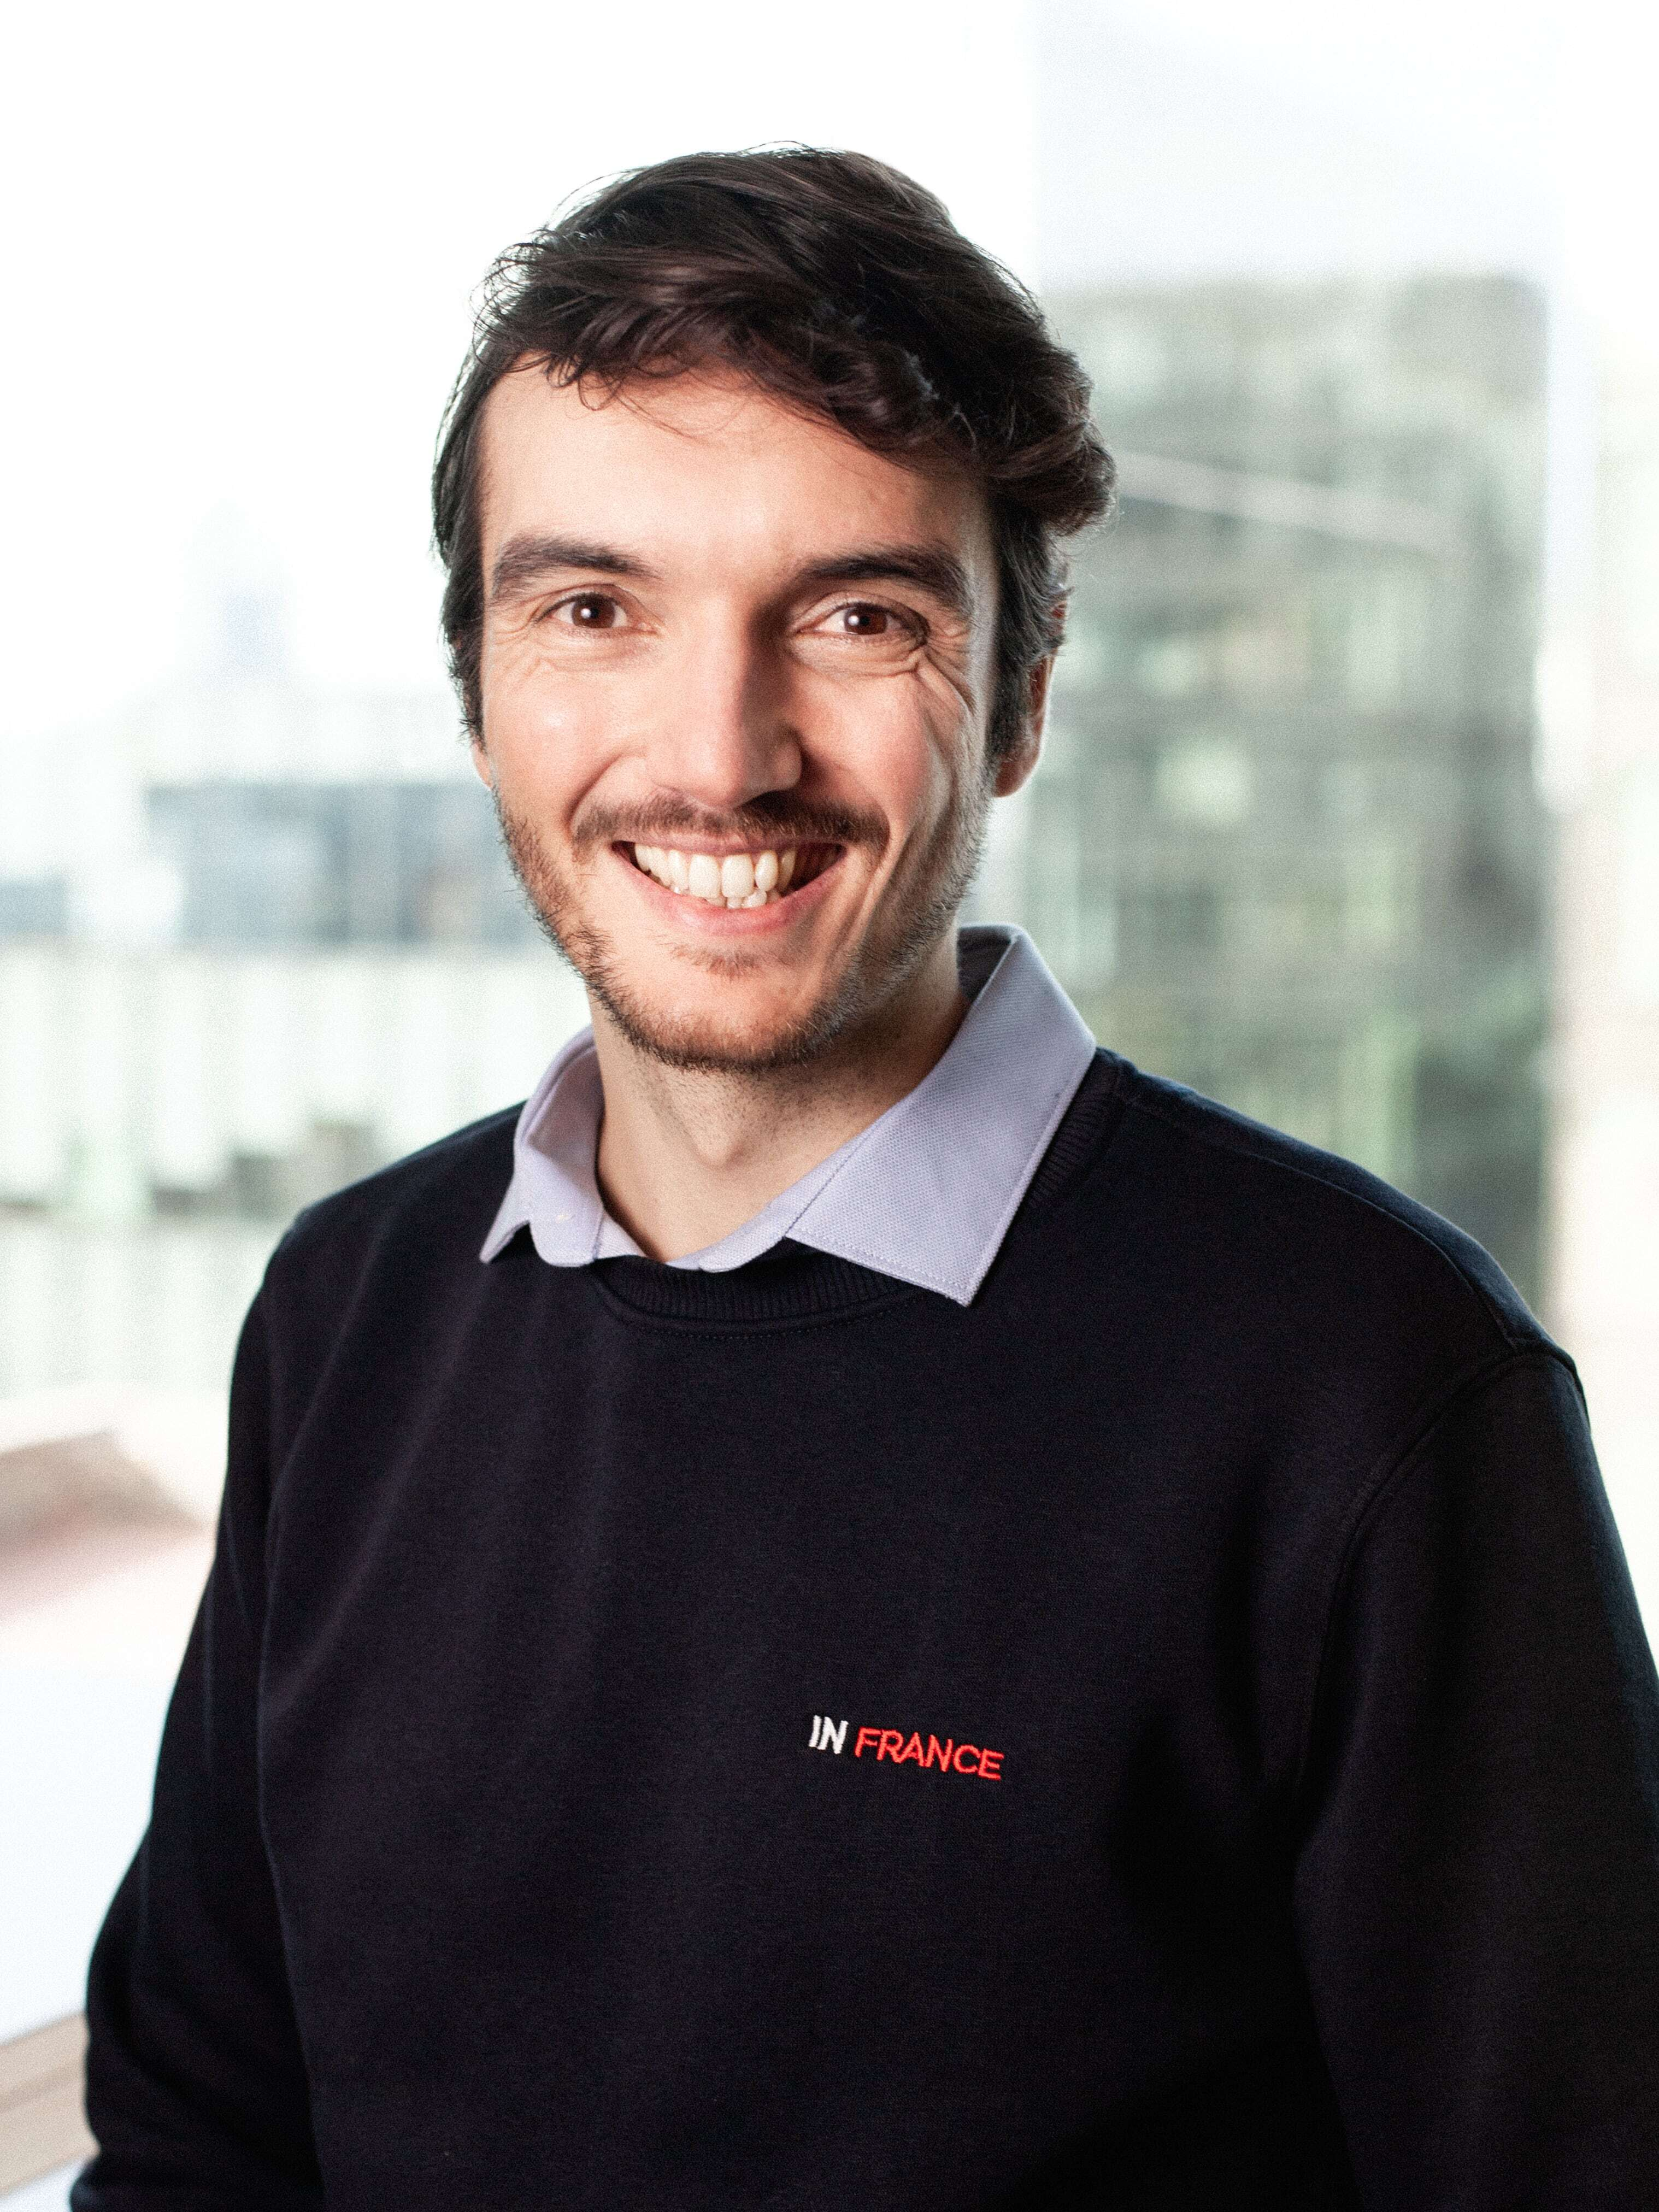
\includegraphics[width=5cm]{image/trombine-christophe}
        \end{columns}
    \end{frame}

    \subsection{Operating System}\label{subsec:os}

    \begin{frame}{Operating System}{Définition de l'OS\footnote{\label{os}C’est quoi un OS (O.S)~?, \url{https://culture-informatique.net/cest-quoi-un-os/}}}
        Un système d'exploitation (OS) est un ensemble de programmes qui gère les ressources matérielles et logicielles d'un ordinateur.
        Il permet également une interaction entre l'utilisateur et l'ordinateur.
        \begin{itemize}
            \item Gère le processeur, la mémoire, les périphériques.
            \item Fournit une interface utilisateur.
            \item Sert d'intermédiaire entre les logiciels et le matériel.
        \end{itemize}
        \bigbreak
        Sans OS, le hardware est inutilisable.
    \end{frame}

    \begin{frame}{Operating System}{Fonctionnement de l'OS\cref{os}}
        L'OS agit comme un intermédiaire entre les logiciels et le matériel.
        Les logiciels ne communiquent pas directement avec le matériel (ou très rarement autorisés par certains OS et sous certaines conditions), mais passent par l'OS~.
        \begin{itemize}
            \item Les logiciels sont installés sur l'OS~.
            \item Les logiciels sont compilés pour un OS spécifique (par exemple, un logiciel pour Windows ne fonctionnera pas sur iOS).
        \end{itemize}
    \end{frame}

    \begin{frame}{Operating System}{Les Pilotes (Drivers)\cref{os}}
        L'OS utilise des pilotes pour communiquer avec les périphériques.
        Un pilote est un programme qui agit comme un traducteur entre l'OS et le matériel.
        \begin{itemize}
            \item Chaque périphérique (souris, clavier, imprimante) a besoin d'un pilote pour fonctionner correctement.
            \item Exemple~: le pilote d'une imprimante traduit les commandes de l'OS en instructions compréhensibles pour l'imprimante.
        \end{itemize}
    \end{frame}

    \begin{frame}{Operating System}{Évolution des OS\cref{os}}
        Historiquement, les premiers OS avaient une interface textuelle ou en ligne de commande, sans interface graphique.
        Quelques exemples d'OS historiques incluent~:
        \begin{itemize}
            \item IBM System/360 Operating System d'IBM~.
            \item Unix.
            \item MSDOS~.
            \item L'évolution vers des interfaces graphiques avec MacOS et Windows.
            \item Aujourd'hui, des OS comme Android dominent sur les smartphones.
        \end{itemize}
    \end{frame}

    \begin{frame}{Operating System}{Conclusion\cref{os}}
        L'OS est la colonne vertébrale de tout appareil informatique.
        Il gère les interactions entre les logiciels et le matériel, tout en offrant une interface pour l'utilisateur.
        Sans un OS, nos appareils modernes ne seraient que des coquilles vides incapables d'exécuter des tâches.
        \bigbreak
        \centering
        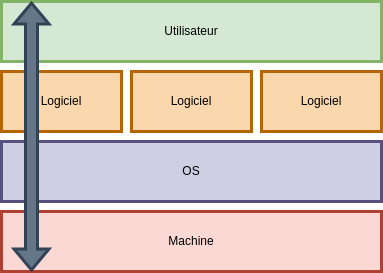
\includegraphics[width=7cm]{image/os.drawio}
    \end{frame}

    \subsection{L'interface utilisateur}\label{subsec:hmi}

    \begin{frame}{L'interface utilisateur}{les principales}
        Les interfaces A.K.A.\ IHM ou \textit{HMI} en anglais ont évolué avec les technologies et les besoins des utilisateurs.
        \begin{itemize}
            \item Les premières interfaces étaient textuelles, comme les terminaux des mainframes IBM et leur IBM System/360 Operating System apparu en 1964\footnote{The IBM System/360, \url{https://www.ibm.com/history/system-360}} et le TSO\footnote{IBM System/360 Operating System: Time Sharing Option Guide, \url{http://bitsavers.informatik.uni-stuttgart.de/pdf/ibm/360/os/R20.1_Mar71/GC28-6698-3_TSO_Option_Guide_Rel_20.1_Jun71.pdf}}.
            Cette interface existe toujours dans les dernières version de ces environnements de type mainframe, aujourd'hui appelé Z/OS~.
            Il y a plus \textit{user friendly} mais la productivité est là.
            \begin{columns}
                \column{0.7\textwidth}
                \item À Palo Alto CA, à Xerox Parc, en 1977, l'Alto de Xerox a des fenêtres avec icônes et une souris~!
                Il ouvre la voie à l'Apple Lisa et Windows.
                \column{0.2\textwidth}
                \begin{center}
                    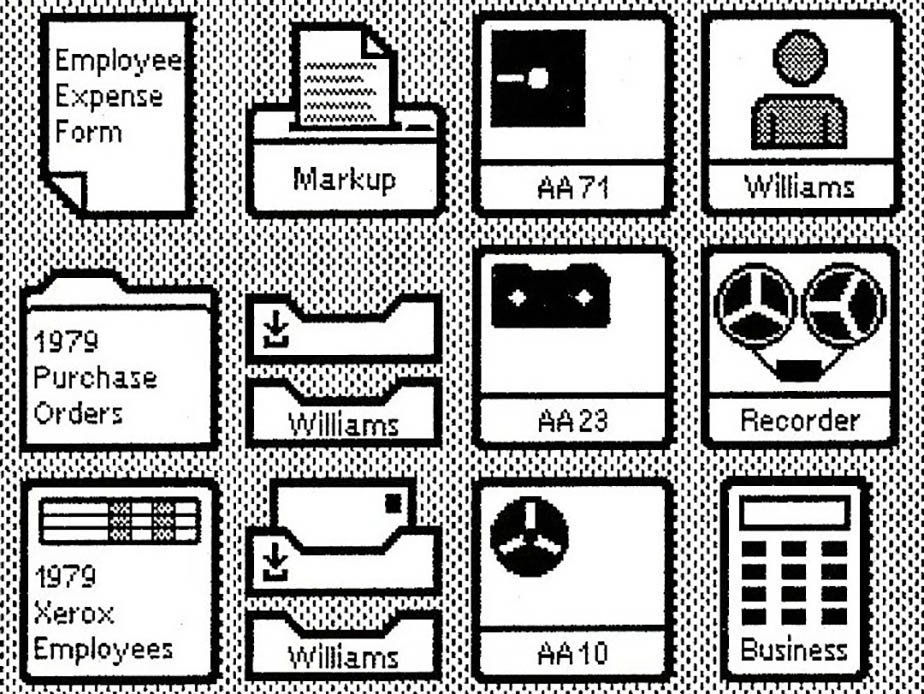
\includegraphics[width=3cm]{image/alto-windows}
                \end{center}
            \end{columns}
        \end{itemize}
    \end{frame}

    \begin{frame}[fragile]{L'interface utilisateur}{les principales}
        \begin{scriptsize}
            \begin{itemize}
                \item Les terminaux en ligne de commandes sont toujours utilisés aujourd'hui, notamment dans les environnements Unix et Linux.
                Ils ont commencé sous Unix, avec K. Thompson et Dennis Ritchie chez Bell Labs (AT\&T) en 1977.
                Cette technologie est portée sous Linux dès son origine et est toujours l'interface de choix pour la connexion à une machine Unix/Linux distante comme un serveur\footnote{\label{ibmunix}UNIX shells since 1977, \url{https://developer.ibm.com/tutorials/l-linux-shells/}}.
                \begin{lstlisting}[language=bash]
$ uname -a
Linux chrichri-HKD-WXX 6.8.0-41-generic #41-Ubuntu SMP PREEMPT_DYNAMIC Fri Aug  2 20:41:06 UTC 2024 x86_64 x86_64 x86_64 GNU/Linux
$ whoami
chrichri
                \end{lstlisting}
                \item Des protocoles de communication comme RDP, VNC permettent de garder l'approche \textit{user friendly} des fenêtres tout en se connectant de manière sécurisée à une machine distante.
                \item Les interfaces tactiles ou la souris est remplacée par un écran tactile.
                Ces interfaces sont principalement portées par les OS destinés aux smartphones et tablettes comme Android, basé sur Linux et iOS, basé sur BSD Unix\footnote{Android adn iOS, \url{https://home.ubalt.edu/abento/315/android-ios/index.html}}.
            \end{itemize}
        \end{scriptsize}
    \end{frame}

    \subsection{Les origines de Unix}\label{subsec:unix-derivatives}
    \begin{frame}{les origines de Unix}{Son histoire\footnote{Brève histoire d'Unix, \url{https://tuteurs.ens.fr/unix/histoire.html}}}
        Le plus proche parent de Linux est Unix.
        Les principaux Unix sont~:
        \begin{itemize}
            \item System V~: Développé par AT\&T en 1983.
            Il donne~:
            \begin{itemize}
                \item AIX~: développé par IBM~.
                \item Solaris~: de Sun Microsystems.
            \end{itemize}
            \item BSD~: Développé par l'Université de Berkeley en 1992.
            Un \textit{rewrite} complet de l'Unix d'AT\&T~.
            Il donne~:
            \begin{itemize}
                \item FreeBSD~: développé à partir 1993.
                \item Toutes les BSD, NetBSD, OpenBSD, \textit{etc}
                \item Mac OS X~: Basé sur Darwin, développé par Apple en 2001.
            \end{itemize}
        \end{itemize}
    \end{frame}

    \begin{frame}{les origines de Unix}{Son histoire}
        Les premières version d'Unix ne sont pas écrites en C mais leur concepteurs vont par la suite développé le langage C et réécrire Unix dans ce langage\cref{ibmunix}.
        \begin{center}
            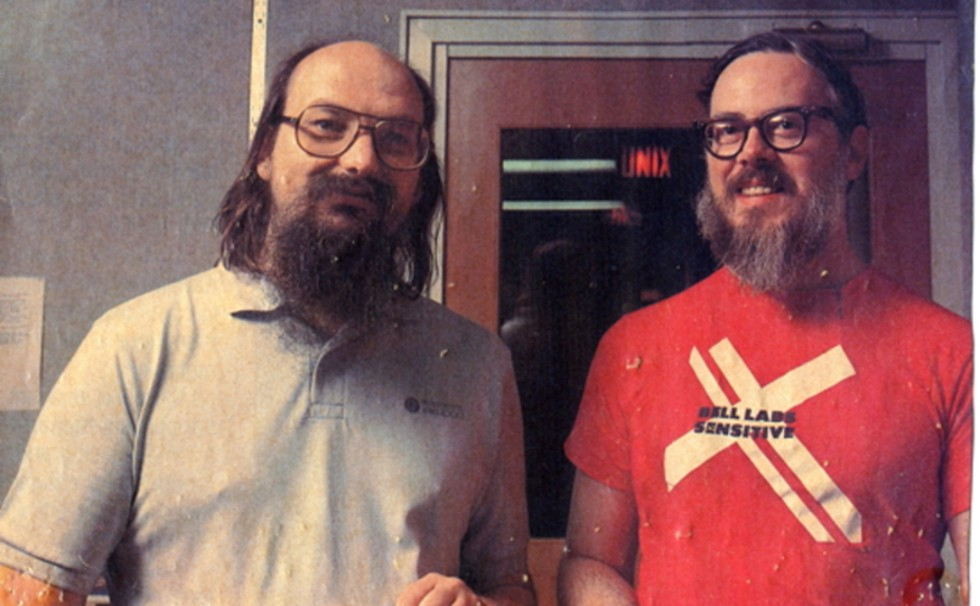
\includegraphics[width=8cm]{image/thompson-rithcie-bell} \\ Ken Thompson et Dennis Ritchie\footnote{Discovering Dennis Ritchie’s Lost Dissertation, \url{https://computerhistory.org/blog/discovering-dennis-ritchies-lost-dissertation/}} \\
        \end{center}
    \end{frame}

    \subsection{Pourquoi Linux~?}\label{subsec:why}

    \begin{frame}{Pourquoi Linux~?}{Les principales raisons}
        \begin{footnotesize}
            \begin{itemize}
                \item Linux est open source, donc peut être gratuit.
                \item Linux est open source, donc son code peut être audité pour vérifier sa sécurité.
                \item Linux est open source et a donc une communauté qui le maintient, le débug et l'améliore constamment.
                \item Linux est une technologie mature qui a un écosystème pouvant répondre à virtuellement à tous les besoins~:
                \begin{itemize}
                    \begin{footnotesize}
                        \item Réseau, FortiOS de Fortinet est basé sur Linux\footnote{\url{https://community.fortinet.com/t5/FortiGate/Technical-Tip-How-to-check-Kernel-version-of-FortiGate/ta-p/323390}}.
                        \item Yocto pour l'embarqué et l'IoT~.
                        \item Les noyaux \textit{RT} pour les systèmes temps réel (automobile, avionique, \textit{etc}).
                        \item Informatique de bureau avec les distributions \textit{user friendly} comme Ubuntu.
                        \item Jeux-vidéo avec Steam OS~.
                        \item 72~806 packages Debian en date du 26 aout 2024\footnote{Debian package management, \url{https://www.debian.org/doc/manuals/debian-reference/ch02.en.html}}.
                        \item \textit{many more}
                    \end{footnotesize}
                \end{itemize}
            \end{itemize}
        \end{footnotesize}
    \end{frame}

    \begin{frame}{Pourquoi Linux~?}{La sécurité}
        \centering
        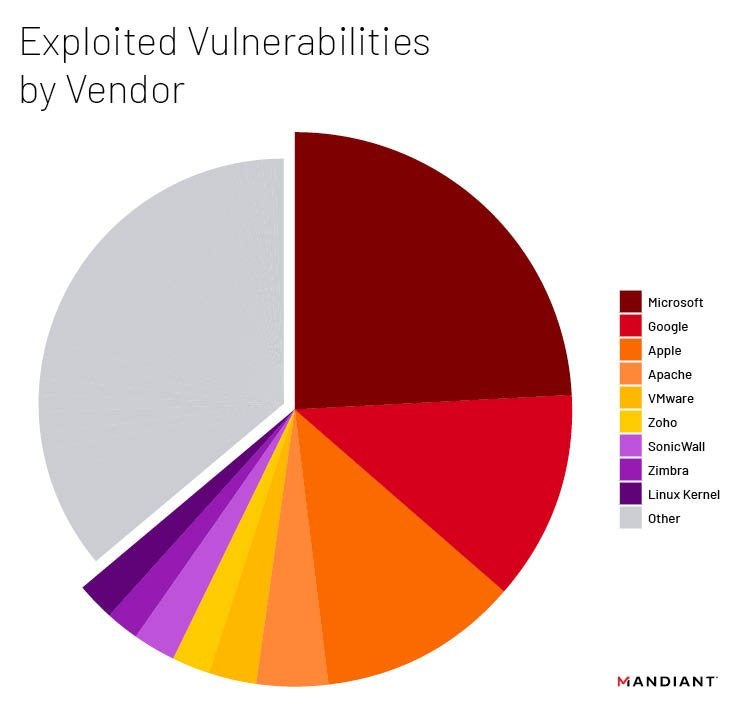
\includegraphics[width=6.5cm]{image/vendors-vuln} \\ Exploited vulnerabilities by vendor\footnote{Analysis of Time-to-Exploit Trends: 2021-2022, \url{https://cloud.google.com/blog/topics/threat-intelligence/time-to-exploit-trends-2021-2022/?hl=en}} \\
    \end{frame}

    \begin{frame}{Pourquoi Linux~?}{L'espionnage}
        Solaris a espionné ses clients, particulièrement les industriels et financiers de Suisse Romande.
        Le développeur Sun Microsystem à disparu\ldots
        \bigbreak
        \begin{columns}
            \centering
            \column{0.2\textwidth}
            
\includegraphics[width=3cm]{image/digicomp-video}
            \column{0.8\textwidth}
            
\includegraphics[width=6cm]{image/Solaris-Logo-2005-500x313} \\ \url{https://www.rts.ch/play/tv/-/video/-?urn=urn:rts:video:12020250} \\
        \end{columns}
    \end{frame}

    \begin{frame}{Pourquoi Linux~?}{Performances\footnote{These Windows 10 Vs Pop OS Benchmarks Reveal A Surprising Truth About Linux Gaming Performance, \url{https://www.forbes.com/sites/jasonevangelho/2019/07/17/these-windows-10-vs-pop-os-benchmarks-reveal-a-surprising-truth-about-linux-gaming-performance/}}}
        Performances proches de celles de Windows, parfois supérieur~!
        \begin{center}
            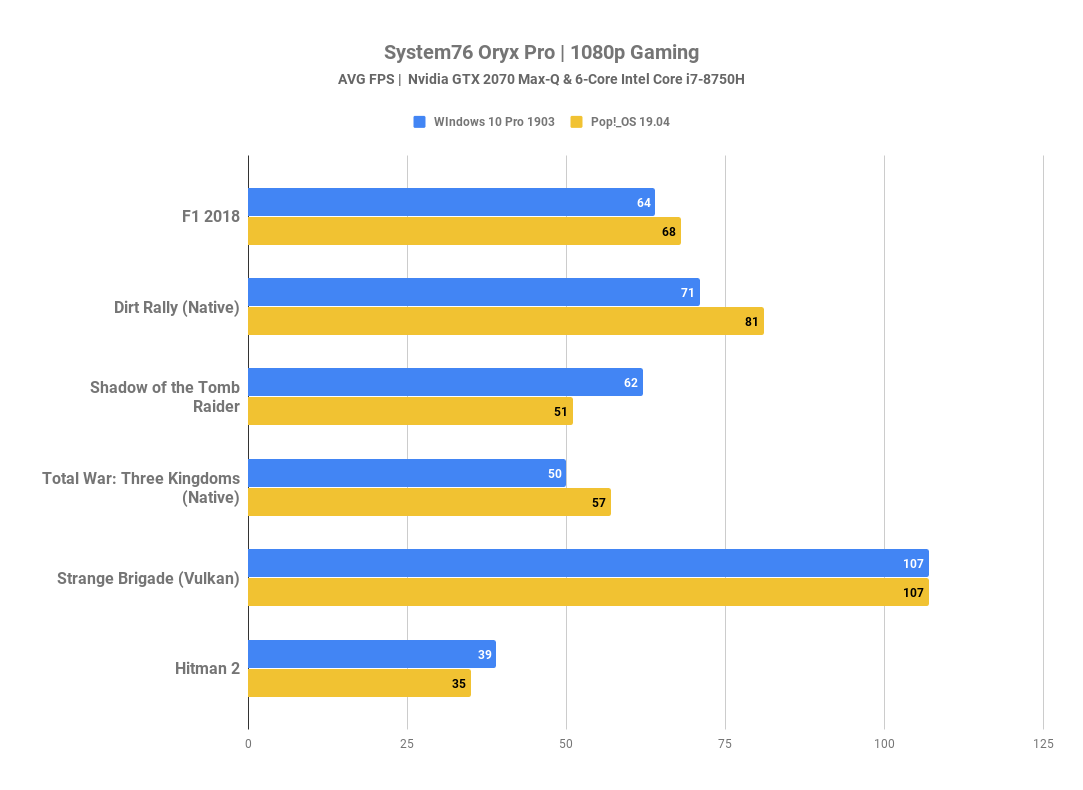
\includegraphics[width=8cm]{image/linux-vs-windows}
        \end{center}
    \end{frame}

    \begin{frame}{Pourquoi Linux~?}{Les architectures supportées\footnote{Statistics per Debian architectures, \url{https://popcon.debian.org/}}}
        \begin{center}
            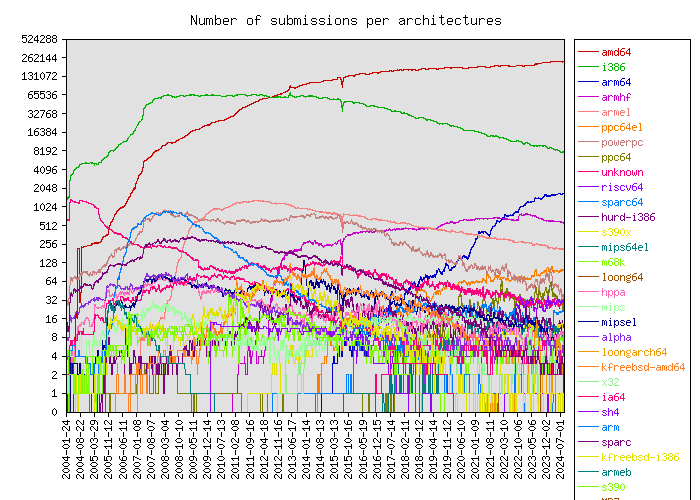
\includegraphics[width=10cm]{image/submission-by-architecture}
        \end{center}
    \end{frame}

    \begin{frame}{Pourquoi Linux~?}{Adoption et impact économique}
        \begin{itemize}
            \item \emoji{flag-switzerland} La Chancellerie fédérale Suisse promeut les avantages de l'open source dans un un guide stratégique adréssé à l'administration\footnote{Administration fédérale et logiciels ouverts, \url{https://www.bk.admin.ch/dam/bk/fr/dokumente/dti/ikt-vorgaben/strategien/oss/Em002_1-0_GENEHMIGT_f.pdf.download.pdf/Em002_1-0_GENEHMIGT_f.pdf}}.
            \item \emoji{flag-france} En France, un marché de 5 milliards par an avec une croissance 7~\%\footnote{Les logiciels libres et open source en France~: où en sommes-nous~?, \url{https://labo.societenumerique.gouv.fr/fr/articles/dossier-les-logiciels-libres-et-open-source-en-france-o\%C3\%B9-en-sommes-nous/}}.
            \item \emoji{flag-european-union} Promotion de l'open source dans l'administration publique en EU\footnote{L'Europe publie un guide sur l'Open Source dans l'administration publique, \url{https://code.gouv.fr/fr/blog/guide-osor-sur-open-source-dans-administration-publique/}}.
        \end{itemize}
    \end{frame}

    \begin{frame}{Pourquoi Linux~?}{Adoption}
        \footnotetext{Why Linux runs 90 percent of the public cloud workload, \url{https://www.cbtnuggets.com/blog/certifications/open-source/why-linux-runs-90-percent-of-the-public-cloud-workload}}
        \footnotetext{\label{cbt}When everything is in the cloud, does the OS matter?, \url{https://www.redhat.com/en/blog/when-everything-cloud-does-os-matter}}
        \footnotetext{20 great years of Linux and supercomputer, \url{https://www.zdnet.com/article/20-great-years-of-linux-and-supercomputers/?ref=itsfoss.com}}
        \begin{columns}
            \column{0.5\textwidth}
            \begin{itemize}
                \item 2018, 90 \% des serveurs du cloud tournent sous Linux\footnotemark.
                \item 2018, 70 \% des serveurs sont déployés dans le cloud\footnotemark.
                \item 2018, 62 \% de l'embarqué\cref{cbt}.
                \item 2012, 95 \% des supercalculateurs\footnotemark.
            \end{itemize}
            \column{0.5\textwidth}
            \centering
            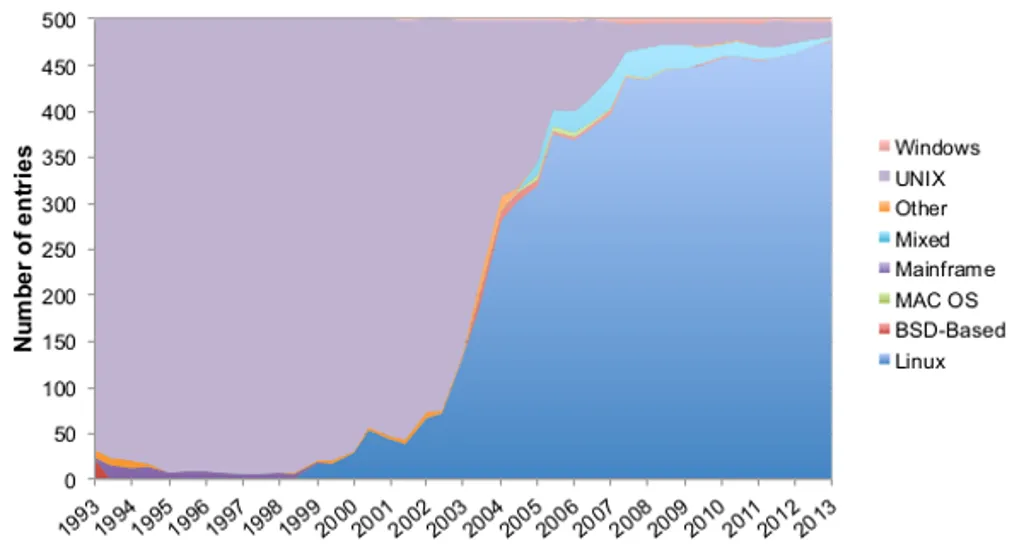
\includegraphics[width=6cm]{image/linux-supercomputer-growth}
        \end{columns}
    \end{frame}

    \subsection{Historique de Linux}\label{subsec:historique}

    \begin{frame}{Historique de Linux}{Linux, quelques caractéristiques de la première version\footnote{The early days of Linux, Lars Wirzenius, \url{https://lwn.net/Articles/928581/}}}
        \begin{footnotesize}
            \begin{itemize}
                \item La première version libérée par Linus Torvald, date de 1991 et sa licence ne permet pas l'usage commercial.
                \item Elle est compilée avec GCC 1.4, A.K.A. \textit{GNU C Compiler} de Richard Stallman.
                La publication de GCC en version 0.9 date de 1987.
                L.~Torvald a déjà porté GCC sous Minix, un OS éducatif\footnote{GCC,\url{https://gunkies.org/wiki/Gcc}}\footnotestep\footnote{A Brief Historu of GCC, \url{https://gcc.gnu.org/wiki/History}}.
                \item 1992, Linux est distribué sous license GNU GPL, donc pour tout usage, même commercial.
                \item 1992, intégration de X11, le serveur graphique, pour favoriser l'usage en \textit{desktop}.
                \item 1993, formation de la communauté Debian.
                \item Fin des années 90, les investissements d'IBM pour supporter Linux atteignent le milliard de dollars\footnote{A strong history and commitment to open source, \url{https://www.ibm.com/opensource/story/}}.
            \end{itemize}
        \end{footnotesize}
    \end{frame}

    \begin{frame}{Historique de Linux}{Historique de tous les OS\footnote{chococigar, \url{https://github.com/chococigar/cup-of-cs/blob/main/img/history\_of\_os.png}}}
        \centering
        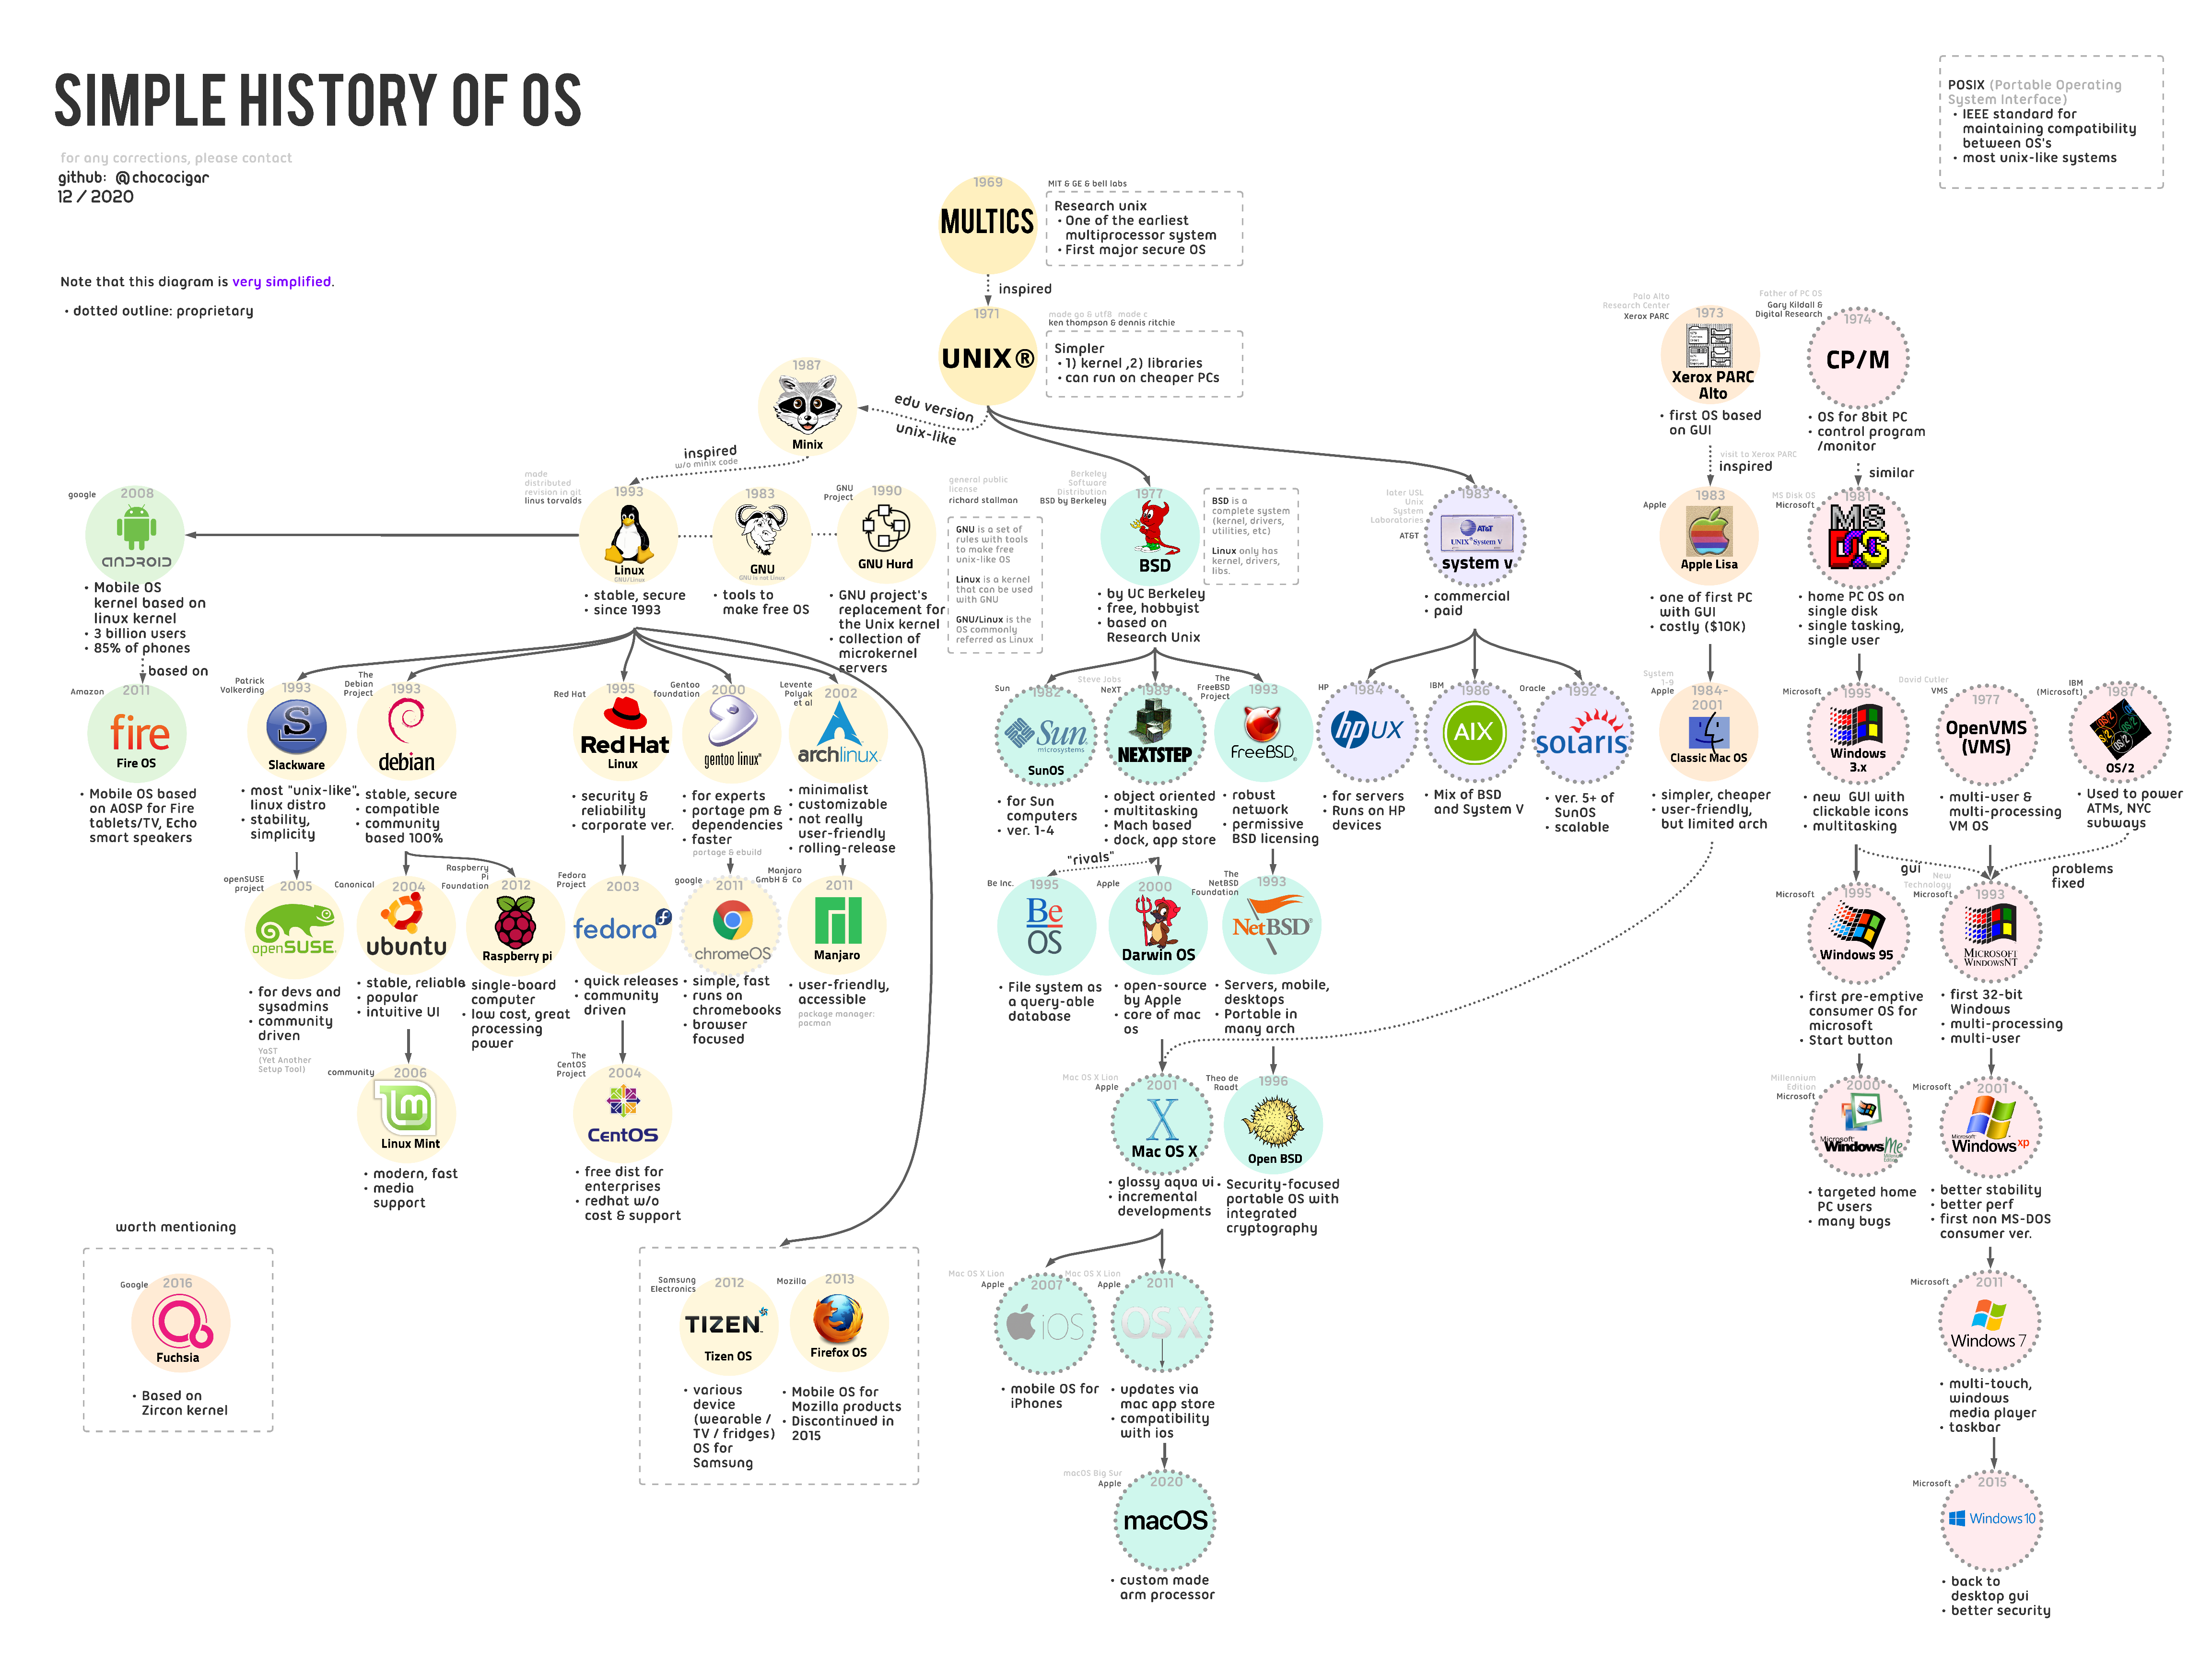
\includegraphics[width=9cm]{image/history_of_os}
    \end{frame}

    \begin{frame}{Historique de Linux}{Linux, historique des single/multi users OS}
        Multi user au sens \textit{Time-Sharing}, \textit{i.e.}, plus d'un utilisateur en même temps.

        Les premiers OS Multi user était OS/360 d'IBM dans les années 60.
        Unix est un concurrent développé par Bell Labs, une filiale d'AT\&T (Avant le démantèlement en 1982), en 1969.

        Linux est ainsi multi user dès le début.
        Par opposition à Windows, qui par défaut (sans RDP ni bricolage), ne l'est pas.
        C'est Windows® Server qui est multi user.
        \bigbreak
        Cette différence est cruciale, car elle a fait de cet OS un candidat idéal pour les serveurs (Web, BDD, \textit{etc}).
    \end{frame}

    \subsection{Kernel et distribution}\label{subsec:kernel-et-distribution}

    \begin{frame}{Les distributions}{Définitions\footnote{Glossary, \url{https://help.ubuntu.com/community/Glossary}}}
        \begin{itemize}
            \item \textbf{Kernel} ou \textbf{Noyau}~: Le composant central d'un système d'exploitation qui contrôle tous les processus bas niveau d'un ordinateur, tels que la gestion de la mémoire, les threads et les entrées/sorties.
            En un sens, le noyau agit comme le gardien de l'ordinateur vis-à-vis du matériel.
            Les applications font des appels système via le noyau pour demander des ressources et interagir avec le matériel.
            \item \textbf{Distribution}~: Désigne une version de GNU/Linux ou d'un autre système d'exploitation open source, bien que certaines personnes soutiennent que le terme devrait inclure les différents systèmes d'exploitation Windows® et Apple.
            Ubuntu est la version la plus populaire, mais il en existe de nombreuses autres, telles que RedHat, qui est bien connue pour les serveurs.
            La plupart des autres distributions sont conçues pour un type particulier d'architecture, comme les téléphones, les netbooks, les routeurs, les serveurs, \textit{etc}.
        \end{itemize}
    \end{frame}

    \begin{frame}{Kernel}{Définition\footnote{Linux fundamentals: user space, kernel space, and the syscalls API surface, \url{https://www.form3.tech/blog/engineering/linux-fundamentals-user-kernel-space}}}
        \centering
        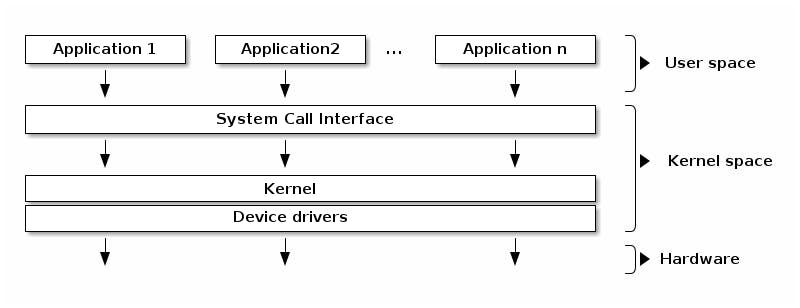
\includegraphics[width=10cm]{image/kernel}
        \flushleft
        \begin{itemize}
            \item \textbf{User space}~: L'espace utilisateur est l'endroit où les applications s'exécutent.
            \item \textbf{Kernel space}~: L'espace noyau est l'endroit où le noyau s'exécute.
            \item \textbf{Syscalls}~: Les appels système sont des interfaces entre les applications et le noyau.
        \end{itemize}
    \end{frame}

    \begin{frame}{Les distributions}{La timeline de toutes les distributions\footnote{FabioLolix, \url{https://github.com/FabioLolix/linuxtimeline}}\footnotestep\footnote{Put the fun back into computing. Use Linux, BSD., \url{https://distributionwatch.com/}}}
        \begin{columns}
            \column{0.8\textwidth}
            Insights~:
            \begin{itemize}
                \item Les 3 plus grosses branches sont Debian, Red Hat et Ubuntu.
                \item Très nombreuses.
                \item Certaines branches meurent même après de longues années d'existence (Mandrake, Centos, \textit{etc}.).
                \item Certaines distributions passent d'une branche à l'autre.
            \end{itemize}
            Quid de l'impact sur la maintenance de la distribution~?
            \column{0.2\textwidth}
            \centering
            \includegraphics[width=1.5cm]{image/linux-all-distro-timeline}
        \end{columns}
    \end{frame}

    \begin{frame}{Les distributions}{La timeline de toutes les distributions}
        Red-Hat, filiale d'IBM, fait l'opposition entre les distributions \textit{entreprise} et les \textit{community}.
        En mettant en avant leur support de 10 ans contre 2 ans pour Fedora, une distribution communautaire de la même branche\footnote{What's the best Linux distribution for you?, \url{https://www.redhat.com/en/topics/linux/whats-the-best-linux-distribution-for-you}}.
        \bigbreak
        Ubuntu a un business model légèrement différent, ils proposent 5 ans de support pour les versions LTS et une extension de 10 ans dans la version payant appelée \textquote{Ubuntu Pro}\footnote{The Ubuntu lifecycle and release cadence, \url{https://ubuntu.com/about/release-cycle}}.
        \bigbreak
        Mais peut-être que l'exemple de Red-Hat n'est pas le bon, Debian, une distribution communautaire également, communique un support des versions LTS de 5 ans minimum\footnote{Debian Long Term Support, \url{https://wiki.debian.org/LTS}}\ldots
    \end{frame}

    \begin{frame}{Les distributions}{La timeline des principales distributions\footnote{\label{main-distribution}Philipp Leclercq, \url{https://github.com/PhilLecl/SanitizedLinuxTimeline}}}
        \centering
        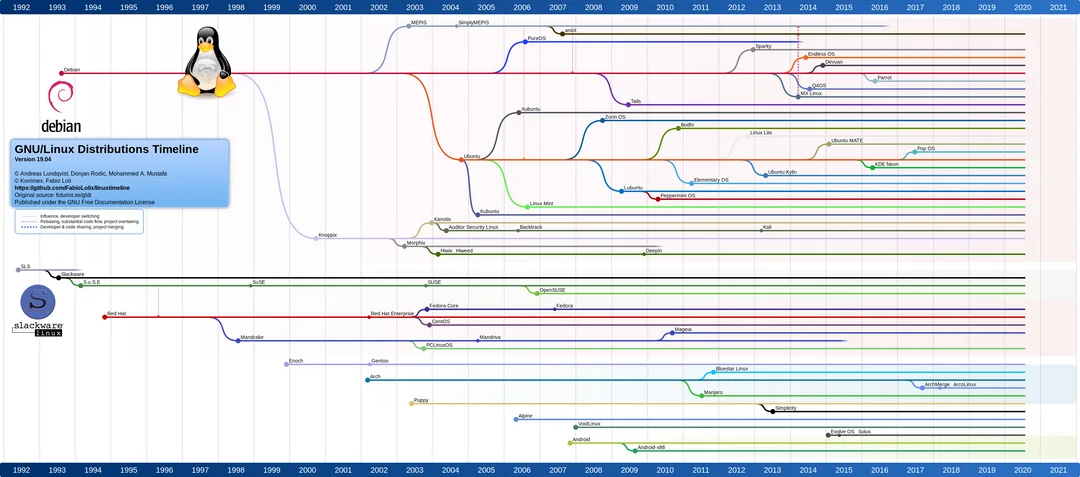
\includegraphics[width=12cm]{image/linux-main-distro-timeline}
    \end{frame}

    \begin{frame}{Les distributions}{Les licences des principales distributions\cref{main-distribution}}
        \centering
        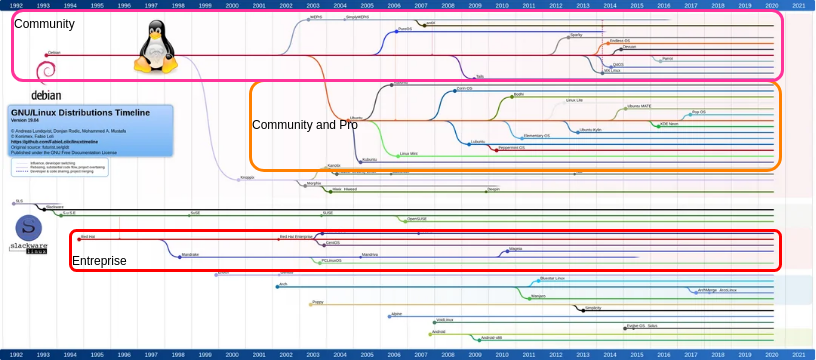
\includegraphics[width=12cm]{image/main-distro-license.drawio}
    \end{frame}

    \begin{frame}{Les distributions}{Les packages managers des principales distributions\cref{main-distribution}}
        \centering
        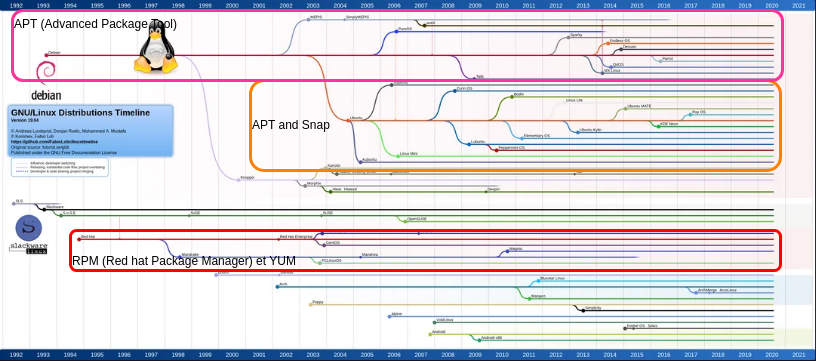
\includegraphics[width=12cm]{image/main-distro-package-manager.drawio}
    \end{frame}

    \begin{frame}{Les distributions}{Une aide pour choisir sa distribution}
        Le site Distrowatch propose un utilitaire pour trouver des distributions candidates en fonction d'un large nombre de critères, \url{https://distrowatch.com/search.php}.
        \bigbreak
        \centering
        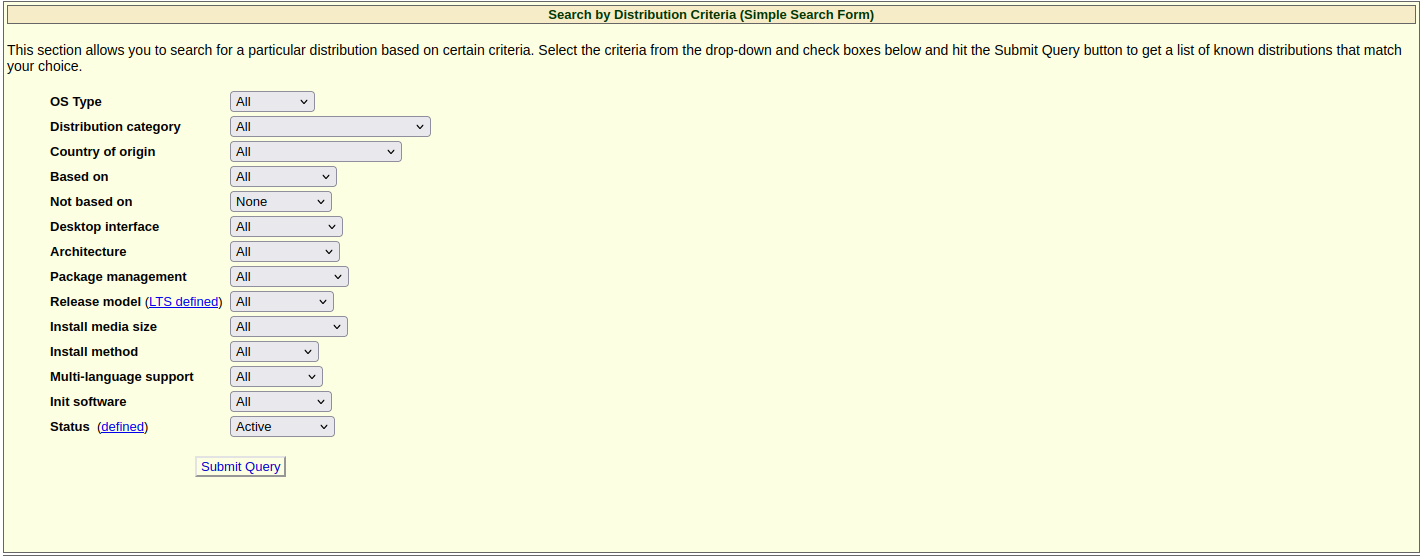
\includegraphics[width=12cm]{image/distrowatch-search}
    \end{frame}

    \begin{frame}{Les distributions}{Une aide pour choisir sa distribution}
        Admettons que tous les 2/3 packages managers mainstreams se valent.
        \bigbreak
        Un des critères différenciant, en plus du support que nous avons vu, est l'architecture.
        \bigbreak
        Qu'est-ce que le critère \textquote{architecture} et pourquoi est-ce important lors d'une migration~?
        \pause
        \bigbreak
        \begin{itemize}
            \item Une modernisation d'un hardware vieillissant qui peut être remplacé par une machine virtuelle faisant tourner les mêmes applications.
            \item Un hardware qui n'est plus supporté par la distribution actuelle et doit donc migrer.
        \end{itemize}
        Dans les 2 exemples, avoir une même architecture permettra ainsi une migration plus \textit{lean}.
        Sans rewrite, voire, sans recompilation.
    \end{frame}

    \begin{frame}{Les distributions}{Des critères manquants~?}
        Y-a-t-il des critères pertinents qui pourraient manquer~?
        \bigbreak
        \centering
        
\includegraphics[width=3cm]{image/question-mark}
    \end{frame}

    \begin{frame}{Les distributions}{Des critères manquants~?}
        L'énorme succès d'une distribution à part, Alpine Linux, poussée par les technologies de virtualisation et de conteneurisation.
        \bigbreak
        Une des premières phrases de présentation sur leur site est \textit{Alpine Linux is built around musl libc and busybox. A container requires no more than 8 MB and a minimal installation to disk requires around 130 MB of storage.}\footnote{About, \url{https://alpinelinux.org/about/}}.
        \bigbreak
        De leur analyse, qui est sûrement la bonne, leur succès vient du compilateur musl et de la librairie C libc musl.
    \end{frame}

    \begin{frame}{Les distributions}{Des critères manquants~?}
        Red-Hat recrute beaucoup d'experts de LLVM ces dernières années\footnote{Red Hat Is Hiring More LLVM Compiler Engineers, \url{https://www.phoronix.com/news/Red-Hat-More-LLVM-Engineers}}.

        Certaines distributions peuvent ou sont compilées avec LLVM comme FreeBSD\footnote{Building FreeBSD with clang/llvm, \url{https://wiki.freebsd.org/BuildingFreeBSDWithClang}}, Chimera\footnote{About Chimera Linux, \url{https://chimera-linux.org/about/}}, OpenMandriva\footnote{La communauté OpenMandriva annonce la disponibilité d'OpenMandriva Lx 4.0, \url{https://linux.developpez.com/actu/266344/La-communaute-OpenMandriva-annonce-la-disponibilite-d-OpenMandriva-Lx-4-0-qui-apporte-de-nombreuses-nouveautes-liees-a-LLVM-Clang/}}\ldots
    \end{frame}

    \begin{frame}{Les distributions}{Plusieurs combinaisons de compilateurs et libraries C}
        \centering
        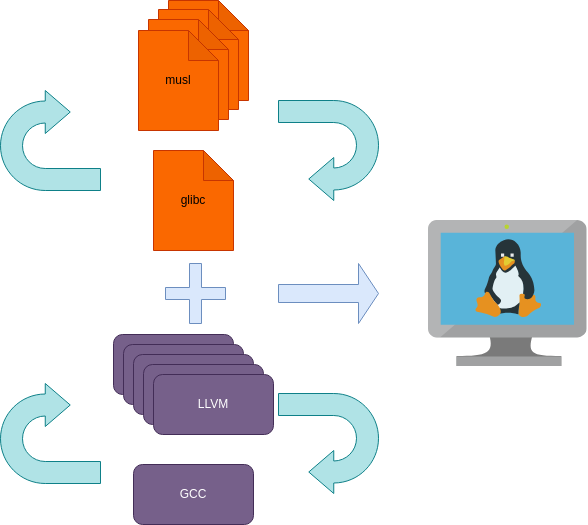
\includegraphics[width=8cm]{image/interchange-lib-compiler.drawio}
    \end{frame}

    \begin{frame}{Les distributions}{Conclusion}
        \begin{columns}
            \column{0.6\textwidth}
            Une distribution Linux est construite de manière modulaire~:
            \begin{itemize}
                \item Version de noyau.
                \item Packages manager.
                \item Architecture.
                \item Licence.
                \item Support.
                \item Librairie C~.
                \item Compilateur.
                \item \textit{Many more}.
            \end{itemize}
            \column{0.4\textwidth}
            \centering
            
\includegraphics[width=5.5cm]{image/craftsman-focused}
        \end{columns}
        \bigbreak
        À vous de trouver la meilleure combinaison pour vos besoins.
    \end{frame}

    \subsection{Quel avenir pour Linux~?}\label{subsec:future-of-linux}

    \begin{frame}{Quel avenir pour Linux~?}
        \begin{columns}
            \column{0.7\textwidth}
            \begin{itemize}
                \item Pas de concurrent dans le Cloud et ce dernier se porte très bien.
                \item Un challenger sur le marché Desktop, grâce à son environnement de plus en plus convivial.
                \item Plus d'instabilité géopolitique et de guerres économiques favorise les solutions ouvertes.
                Car on ne sait pas si la propriété intellectuel pourra poser des soucis de production à l'avenir.
                Thalès passe des appels d'offres sur les plateforme ouvertes comme RISC-V~.
                \item 1 seul concurrent sur le mobile.
                \item De plus en plus de Rust pour améliorer la sécurité et les performances.
                \item Windows intègre Linux avec les WSL~.
            \end{itemize}
            \column{0.3\textwidth}
            \centering
            
\includegraphics[width=4cm]{image/pinguin-fortune-teller}
        \end{columns}
        \bigbreak
        Pas de raison de s'inquiéter~!
    \end{frame}


    \section{Premiers pas}\label{sec:first-step}

    \subsection{Login et Logout}\label{subsec:login-logout}

    \begin{frame}{Login et Logout}
        Lors de l'installation, on définit l'identifiant d'un utilisateur avec les droits administrateurs aussi appelé superutilisateur.
        Souvent cet utilisateur est appelé \lstinline{root} et ne peut être changé.
        \bigbreak
        Ce superutilisateur pourra par la suite créer d'autres utilisateurs et superutilisateurs.
        \bigbreak
        En fonction de la distribution utilisée, les paramétrages initiaux se font dans une interface graphique ou dans une interface textuelle.

        Si c'est une distribution pour les serveurs/le cloud, elle favorise la performance et la légèreté avec une simple interface textuelle.

        Des interfaces d'installation plus conviviales existent pour le desktop.
    \end{frame}

    \begin{frame}{Login et Logout}{Les fenêtres}
        \centering
        
\includegraphics[width=10cm]{image/Ubuntu-login-screen} \\ Connexion sur un Ubuntu Desktop ou Remote Desktop \\
    \end{frame}

    \begin{frame}{Login et Logout}{Les fenêtres}
        \centering
        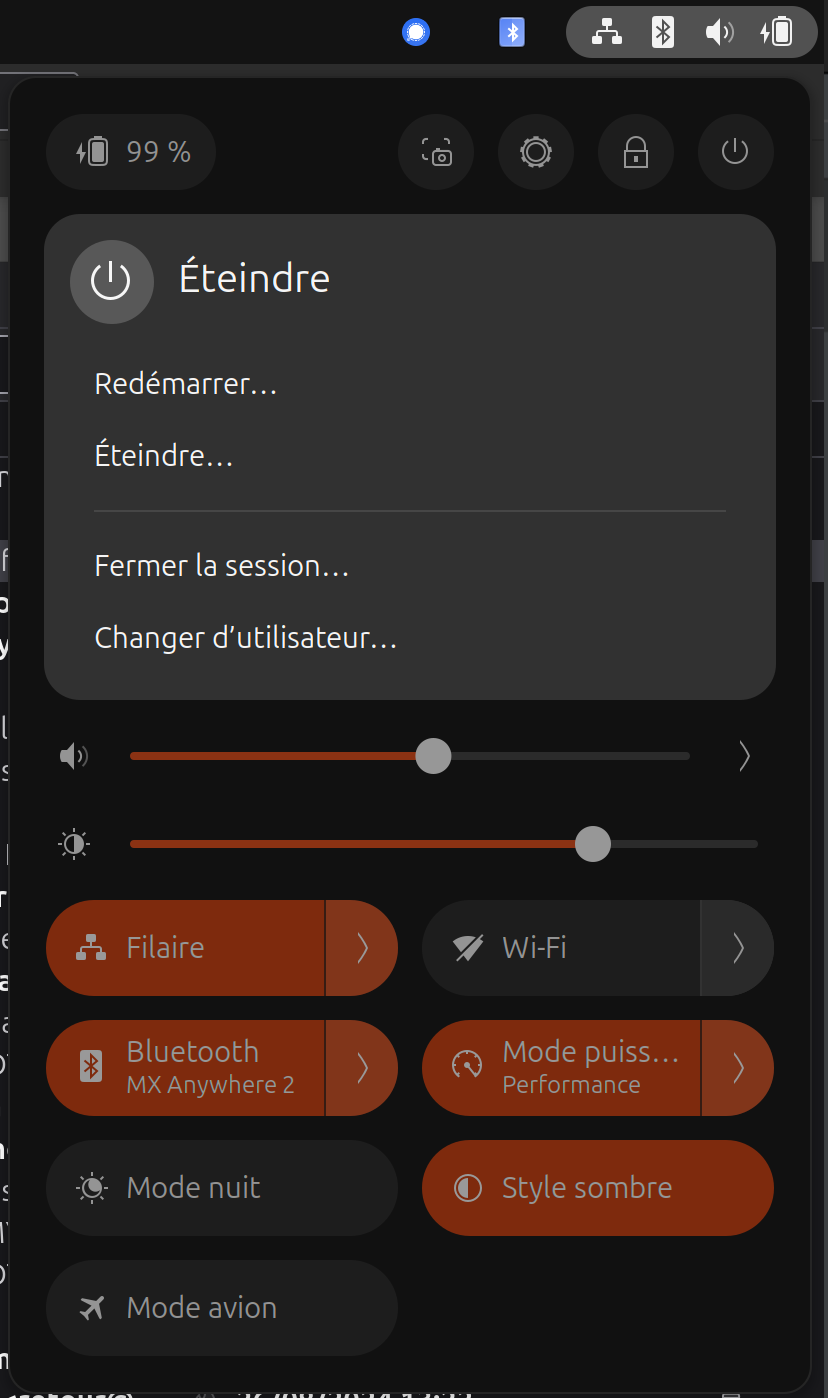
\includegraphics[width=5cm]{image/Ubuntu-logout-screen} \\ Options de déconnexion Ubuntu Desktop ou Remote Desktop \\
    \end{frame}

    \begin{frame}[fragile]{Login et Logout}{Le terminal}
        \begin{lstlisting}[language=bash,basicstyle=\tiny\ttfamily]
$ shutdown --help
shutdown [OPTIONS...] [TIME] [WALL...]

Shut down the system.

Options:
     --help      Show this help
  -H --halt      Halt the machine
  -P --poweroff  Power-off the machine
  -r --reboot    Reboot the machine
  -h             Equivalent to --poweroff, overridden by --halt
  -k             Don't halt/power-off/reboot, just send warnings
     --no-wall   Don't send wall message before halt/power-off/reboot
  -c             Cancel a pending shutdown
     --show      Show pending shutdown

This is a compatibility interface, please use the more powerful 'systemctl reboot',
'systemctl poweroff', 'systemctl reboot' commands instead.

See the shutdown(8) man page for details.
$ shutdown -h
Shutdown scheduled for Wed 2024-08-28 14:49:23 CEST, use 'shutdown -c' to cancel.
$ shutdown -c
        \end{lstlisting}
    \end{frame}

    \subsection{Gérer des fichiers et des répertoires avec la souris}\label{subsec:manage-files-and-directories-with-mouse}

    \begin{frame}{Gestionnaires de fichiers\footnote{Gestionnaires de fichiers, \url{https://doc.ubuntu-fr.org/gestionnaire_de_fichiers}}}
        Il existe de nombreux gestionnaires de fichiers sous Linux.

        \begin{itemize}
            \item  \href{https://doc.ubuntu-fr.org/dolphin}{Dolphin}~: le gestionnaire de fichiers par défaut de Kubuntu (KDE4)
            \item  \href{https://doc.ubuntu-fr.org/konqueror}{Konqueror}~: gestionnaire de fichiers KDE très complet
            \item  \href{https://doc.ubuntu-fr.org/nautilus}{Nautilus}~: le gestionnaire de fichiers par défaut d'Ubuntu (Gnome)
            \item  \href{https://doc.ubuntu-fr.org/nemo}{Nemo}~: fork de Nautilus et gestionnaire de fichiers par défaut du bureau Cinnamon (depuis la version 1.6)
            \item  \href{https://doc.ubuntu-fr.org/pcmanfm}{PCMan File Manager}~: gestionnaire de fichiers léger
            \item  \href{https://doc.ubuntu-fr.org/spacefm}{SpaceFM}~: fork de PCMan File Manager
            \item  \href{https://doc.ubuntu-fr.org/thunar}{Thunar}~: le gestionnaire de fichiers par défaut de Xubuntu
            \item  \href{https://doc.ubuntu-fr.org/caja}{Caja}~: le gestionnaire de fichiers de \href{https://doc.ubuntu-fr.org/mate}{Ubuntu MATE}
            \item  \href{https://doc.ubuntu-fr.org/peony}{Peony}~: le gestionnaire de fichiers de \href{https://doc.ubuntu-fr.org/ukui}{UKUI}
        \end{itemize}
    \end{frame}

    \begin{frame}{Gestionnaires de fichiers}
        Vérifions que Ubuntu utilise bien Nautilus comme gestionnaire de fichiers.
        \bigbreak
        \begin{columns}
            \column{0.5\textwidth}
            \centering
            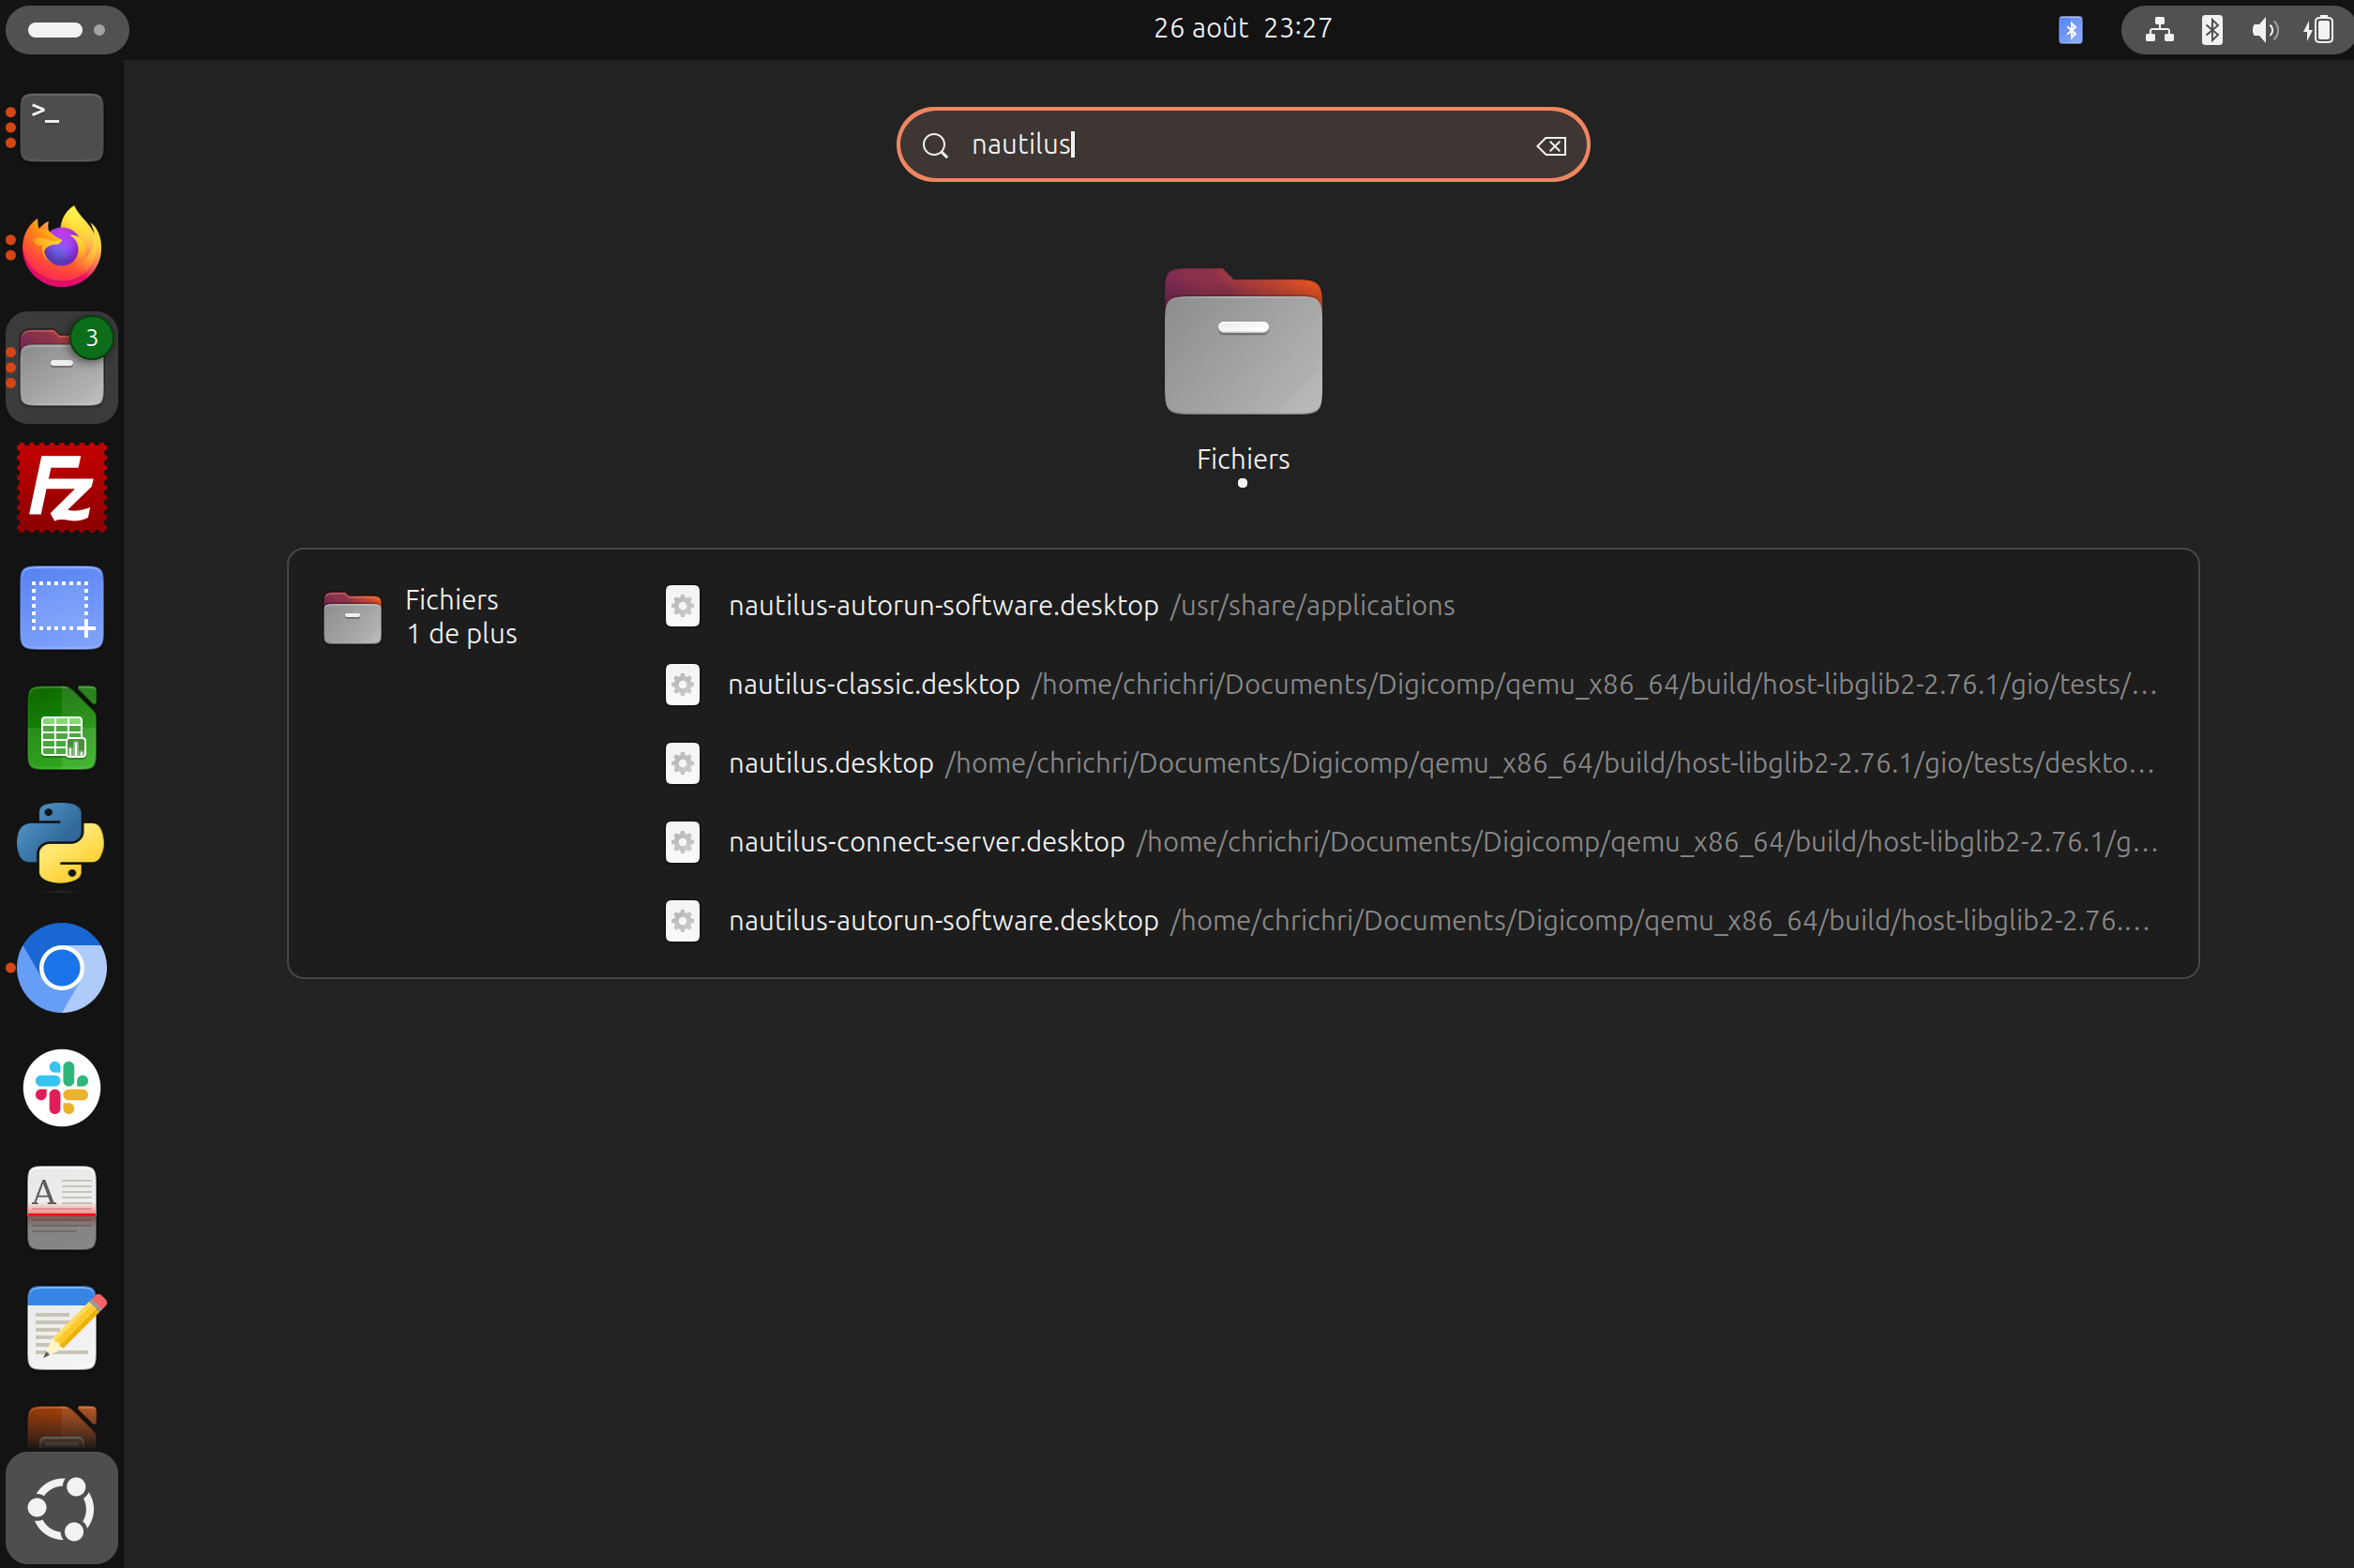
\includegraphics[width=5cm]{image/nautilus-gui} \\ Nautilus est bien trouver par le launcher \\
            \column{0.5\textwidth}
            \centering
            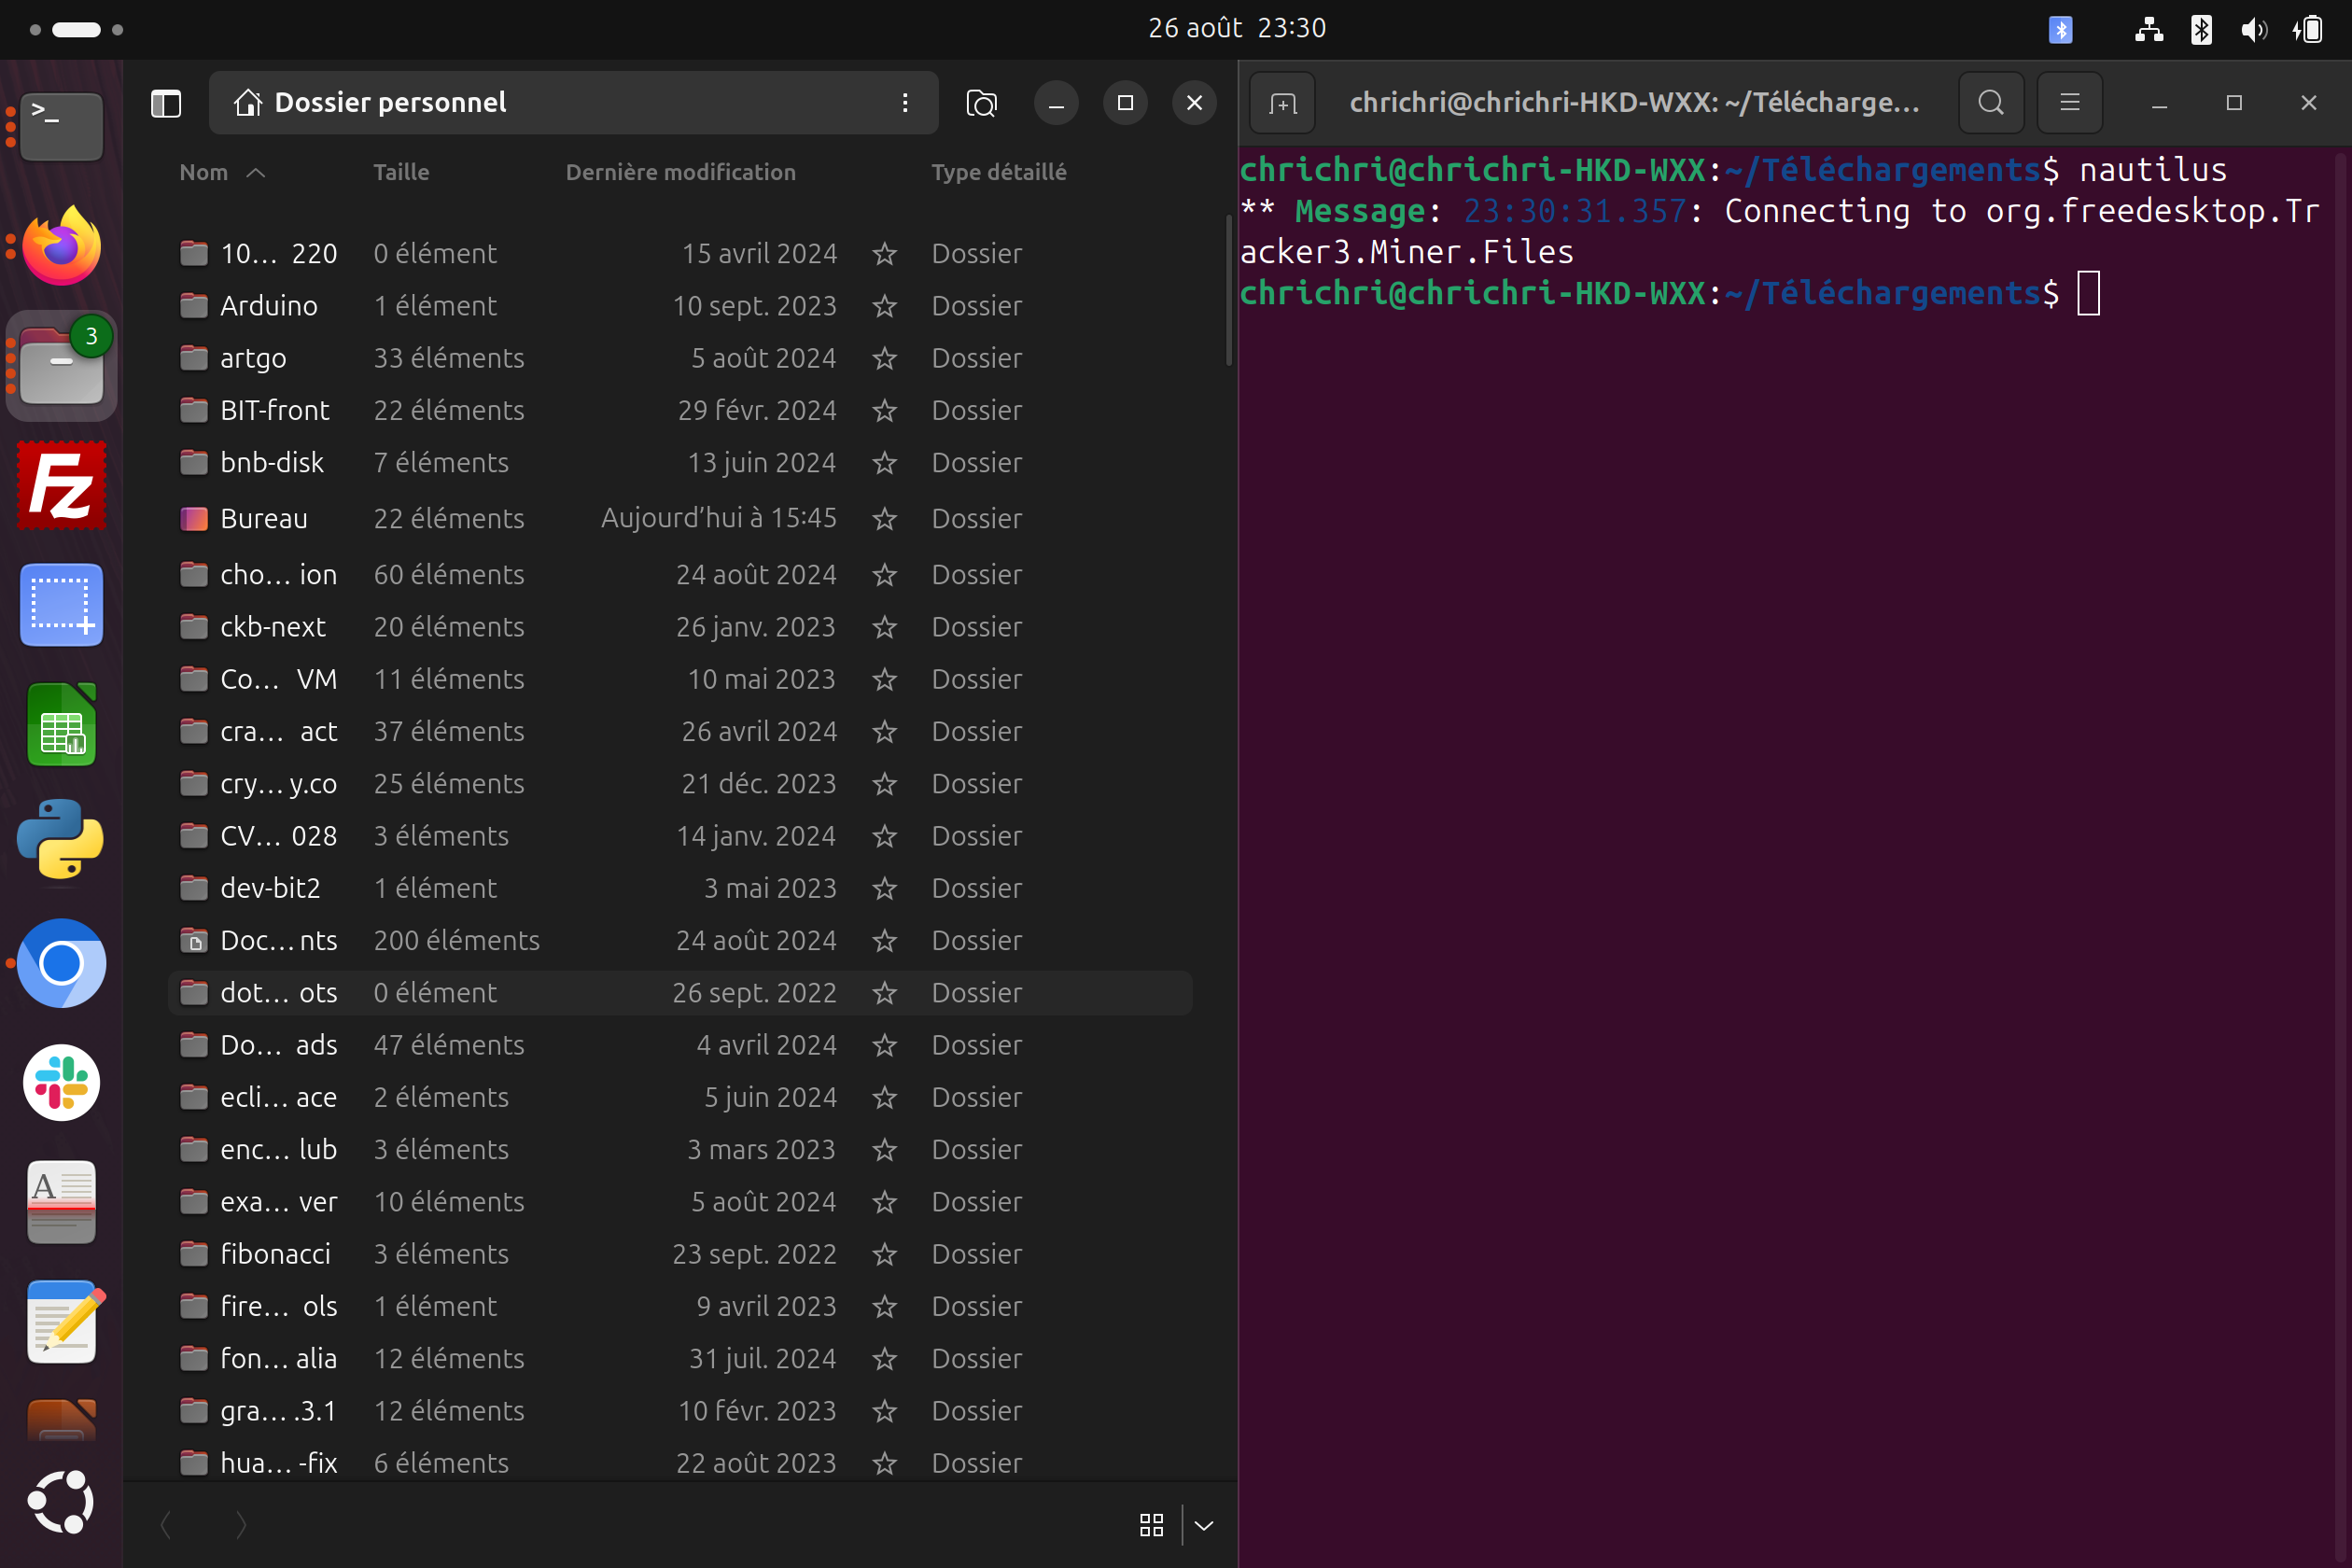
\includegraphics[width=5cm]{image/nautilus-cli} \\ Le gestionnaire se lance quand on lance la commande \lstinline{nautilus} \\
        \end{columns}
    \end{frame}

    \begin{frame}[fragile]{Gestionnaires de fichiers}
        Il n'existe pas sous une version serveur~:
        % bash listing
        \begin{lstlisting}[language=bash]
$ nautilus

La commande « nautilus » n'a pas été trouvée, mais peut être installée avec~:

$ sudo apt install nautilus
        \end{lstlisting}
        Il faut naviguer avec les commandes du terminal A.K.A.\ le Shell.
        \begin{itemize}
            \item \lstinline{ls}~: Liste les fichiers et répertoires.
            \item \lstinline{cd}~: Change de répertoire.
            \item \lstinline{pwd}~: Affiche le répertoire courant.
            \item \lstinline{cp}~: Copie des fichiers et des répertoires.
            \item \lstinline{mv}~: Déplace des fichiers et des répertoires.
            \item \lstinline{rm}~: Supprime des fichiers et des répertoires.
            \item \lstinline{mkdir}~: Crée des répertoires.
            \item \lstinline{touch}~: Crée des fichiers.
        \end{itemize}
        Pas de commande de renommage par défaut il faut l'installer.
    \end{frame}

    \begin{frame}[fragile]{La commande \lstinline{ls}}
        La commande \lstinline{ls} permet de lister les fichiers et répertoires.
        Sous forme de liste avec l'option \lstinline{l}, tous les fichiers y compris les cachés avec l'option \lstinline{a} et de manière \textit{human readable} avec l'option \lstinline{h}.
        \lstinline{/} est le chemin dont il faut lister le contenu.
        Il peut être un dossier ou fichier, si c'est un fichier seul ce fichier sera listé.
        \begin{lstlisting}
$ ls -lha /
total 92K
drwxr-xr-x  23 root     root     4,0K août  17 15:20 .
drwxr-xr-x  23 root     root     4,0K août  17 15:20 ..
drwxr-xr-x   4 root     root     4,0K août  24 00:10 boot
drwxr-xr-x  20 root     root     5,9K août  26 22:11 dev
drwxr-xr-x 198 root     root      12K août  23 15:16 etc
drwxr-xr-x   5 root     root     4,0K août  16 14:35 home
drwxr-xr-x   4 root     root     4,0K août  17 15:44 mnt
drwxr-xr-x  10 root     root     4,0K mai   23 10:34 opt
dr-xr-xr-x 459 root     root        0 août  26 10:03 proc
drwx------  21 root     root     4,0K août  18 23:08 root
drwxr-xr-x  49 root     root     1,5K août  26 22:29 run
drwxr-xr-x   2 root     root     4,0K août  19  2021 srv
dr-xr-xr-x  13 root     root        0 août  26 10:03 sys
        \end{lstlisting}
    \end{frame}

    \begin{frame}[fragile]{Les chemins}
        Les chemins ou \textit{paths} en anglais sont des adresses pour accéder à des fichiers ou des répertoires.
        Ils sont relatifs ou absolus~:
        \bigbreak
        \begin{columns}
            \column{0.7\textwidth}
            \begin{itemize}
                \item \textbf{Relatif}~: Par rapport au répertoire courant.
                \item \textbf{Absolu}~: Par rapport à la racine \lstinline{/}.
                \item \textbf{Parent}~: \lstinline{..} pour remonter d'un répertoire.
                \item \textbf{Home}~: \lstinline{~} pour accéder au répertoire de l'utilisateur courant.
                \item \textbf{Courant}~: \lstinline{.} pour le répertoire courant.
            \end{itemize}
            \column{0.3\textwidth}
            \centering
            
\includegraphics[width=4cm]{image/tux-path}
        \end{columns}
    \end{frame}

    \begin{frame}[fragile]{Les chemins}
        Afficher mon \textit{home}~:
        \begin{lstlisting}
$ ls -lha ~
total 1,9G
drwxr-xr-x 145 chrichri chrichri  12K août  27 09:26  .
drwxr-xr-x   5 root     root     4,0K août  16 14:35  ..
drwxrwxr-x   2 chrichri chrichri 4,0K avril 15 22:42  103.164.116.220
drwxrwxr-x   3 chrichri chrichri 4,0K mai   12 23:28  .anaconda
...
        \end{lstlisting}
        Le contenu du répertoire parent~:
        \begin{lstlisting}
$ ls -lha ..
total 76K
drwxrwxr-x 3 chrichri chrichri 4,0K août  27 10:19 .
drwxrwxr-x 9 chrichri chrichri 4,0K août  26 14:36 ..
drwxrwxr-x 2 chrichri chrichri 4,0K août  27 09:58 image
-rw-rw-r-- 1 chrichri chrichri  61K août  27 10:19 linux.tex
        \end{lstlisting}
        Un fichier du répertoire parent~:
        \begin{lstlisting}
$ ls -lha ../linux.tex
-rw-rw-r-- 1 chrichri chrichri 62K août  27 10:21 ../linux.tex
        \end{lstlisting}
    \end{frame}

    \begin{frame}{Les chemins}{Exercice \execcounterdispinc}
        \begin{itemize}
            \item Lister tous les fichiers de votre \textit{home}.
            \item Lister tous les fichiers du répertoire \lstinline{/etc}.
            \item Lister un fichier du répertoire parent du parent.
            \item Lister un fichier d'un répertoire enfant.
        \end{itemize}
        \begin{center}
            
\includegraphics[width=3cm]{image/question-mark}
        \end{center}
    \end{frame}

    \begin{frame}{Gestion des chemins et des répertoires}{Exercice \execcounterdispinc}
        \begin{enumerate}
            \item Créer un répertoire \lstinline{test} dans votre répertoire personnel.
            \item Créer un fichier \lstinline{test.txt} dans ce répertoire.
            \item Déplacer-vous dans le répertoire \lstinline{test}.
            \item Afficher le contenu du répertoire.
            \item Remonter d'un répertoire.
            \item Afficher le contenu du répertoire.
            \item Supprimer le répertoire \lstinline{test} et son contenu.
        \end{enumerate}
    \end{frame}


    \begin{frame}[fragile]{Changer de répertoire}
        La commande \lstinline{cd} permet de changer de répertoire.

        \lstinline{cd} comme \textit{Change Directory}.
        \begin{lstlisting}[language=bash,basicstyle=\tiny\ttfamily]
$ pwd
/home/chrichri/Documents/Digicomp/Linux/doc/image
$ cd ..
$ ls -l
*total 68
drwxrwxr-x 2 chrichri chrichri  4096 août  27 09:58 image
-rw-rw-r-- 1 chrichri chrichri 64104 août  27 10:59 linux.tex
$ ls /etc/
acpi                           calendar              dbus-1...
chrichri@chrichri-HKD-WXX:~/Documents/Digicomp/Linux/doc$ ls /etc/systemd/system
 acpid.path                                   hibernate.target.wants...
$ cd /etc/systemd/system
$ pwd
/etc/systemd/system
        \end{lstlisting}
        Quel est l'intérêt de la commande \lstinline{cd} puisqu'en comprenant et connaissant les chemins de la machine on peut lancer n'importe quelle commande de n'importe où~?
        \pause
        \begin{itemize}
            \item Pour éviter de taper des chemins absolus ou relatifs trop long.
            \item Si un programme ou script doit s'exécuter dans un chemin donné.
        \end{itemize}
    \end{frame}

    \subsection{Editer des données sans \lstinline{vi}}\label{subsec:edit-whithout-vi}


    \begin{frame}{Editer des données sans \lstinline{vi}}{Les différents éditeurs}
        Une distribution Ubuntu type cloud/server de base a comme éditeur~:
        \begin{itemize}
            \item \lstinline{nano}: Un éditeur de texte simple sous licence GNU~.
            \item \lstinline{vi}: Un éditeur de texte plus complexe et plus puissant.
            Mais il est nécessaire de mémoriser un grand nombre de commandes pour les diverses opérations.
            \item \lstinline{ed}: Un éditeur minimaliste.
            Il nécessite aussi de connaître plusieurs commandes.
            Mais est utile pour éditer des configurations sur des distributions minimalistes ou en mode recovery.
        \end{itemize}
    \end{frame}

    \subsubsection{nano}\label{subsubsec:nano}
    \begin{frame}{Editer des données sans \lstinline{vi}}{Présentation de \lstinline{nano}\footnote{\label{nano}GNU nano, \url{https://www.nano-editor.org/}}}
        \begin{itemize}
            \item \lstinline{nano} est un éditeur de texte simple et facile à utiliser.
            Toutes les commandes sont à l'écran.
            \item Il est souvent installé par défaut sur les systèmes Linux.
            \item Il est idéal pour les débutants ou pour les utilisateurs qui n'ont pas besoin de fonctionnalités avancées.
            \item Coloration syntaxique par défaut, supportant de nombreux langages.
            On peut voir la liste dans le fichier \lstinline{/usr/share/nano/}.
            \item Pour ouvrir un fichier, qu'il existe ou non, la commande est \lstinline{nano <chemin du fichier>}.
        \end{itemize}
        Exercice \execcounterdispinc~: Quels langages sont supportés par votre \lstinline{nano}~?

        Exercice \execcounterdispinc~: Modifier avec \lstinline{nano} la description dans la configuration d'un service du chemin \lstinline{/etc/systemd/system}.
    \end{frame}

    \begin{frame}{Editer des données sans \lstinline{vi}Présentation de \lstinline{nano}}
        \centering
        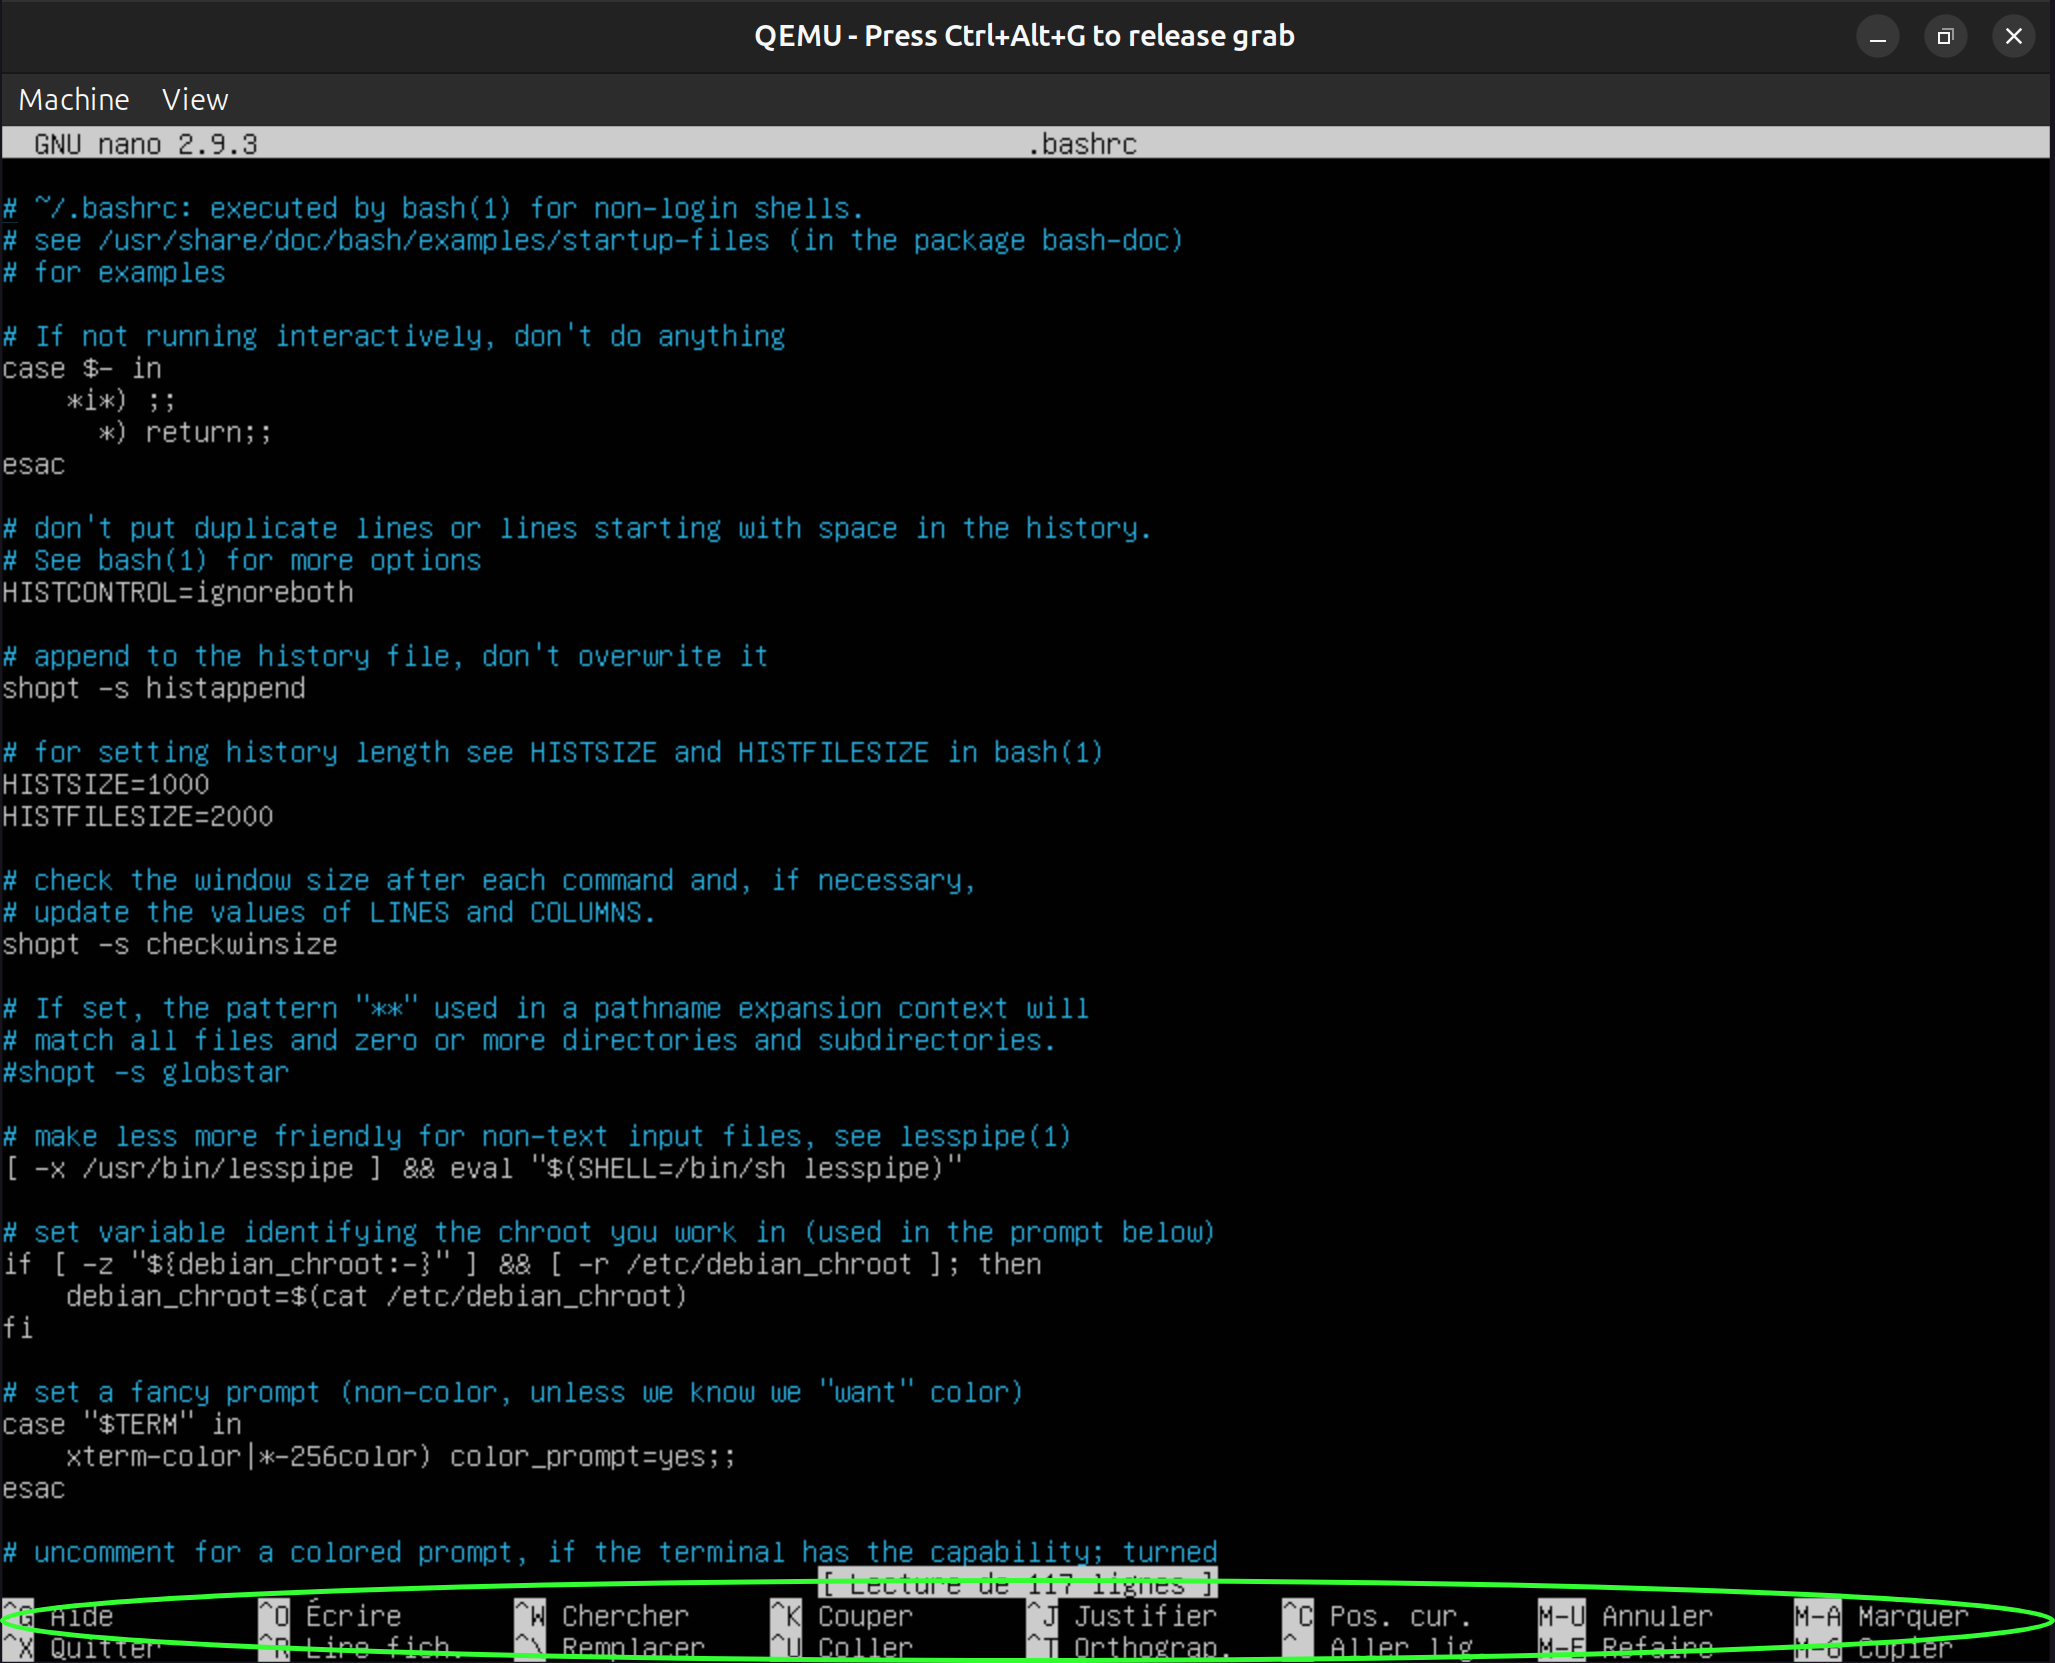
\includegraphics[width=9cm]{image/nano-screen.drawio} \\ Interface de \lstinline{nano}, les commandes sont bas et il y en a 16 seulement! \\
    \end{frame}

    \subsubsection{ed}\label{subsubsec:ed}
    \begin{frame}{Editer des données sans \lstinline{vi}}{Présentation de \lstinline{ed}\footnote{\label{redhated}How to get started with the ed text editor, \url{https://www.redhat.com/sysadmin/introduction-ed-editor}}}
        \begin{itemize}
            \item \lstinline{ed} est l'un des premiers éditeurs de texte Unix.
            \item C'est un éditeur en ligne de commande, sans interface graphique.
            \item Il fonctionne de manière interactive ou par script.
            \item L'éditeur utilise une \textquote{mémoire tampon} pour modifier les fichiers.
        \end{itemize}
    \end{frame}

    \begin{frame}{Editer des données sans \lstinline{vi}}{Lancement de \lstinline{ed}\cref{redhated}}
        \begin{itemize}
            \item Taper simplement \lstinline{ed} pour lancer l'éditeur.
            \item L'éditeur ne fournit pas de retour immédiat ; il attend vos commandes.
            \item Utiliser la commande \lstinline{p} pour afficher un prompt~: \lstinline{?}.
        \end{itemize}
    \end{frame}

    \begin{frame}[fragile]{Editer des données sans \lstinline{vi}}{Ajout et modification de texte avec \lstinline{ed}\cref{redhated}}
        \begin{itemize}
            \item Utiliser la commande \lstinline{a} pour ajouter du texte à la mémoire tampon.
            \item Terminer l'édition avec un point seul sur une ligne \lstinline{.} pour retourner au mode commande.
            \item Exemple~:
            \begin{lstlisting}
a
[myconfig]
widget=True
.
            \end{lstlisting}
        \end{itemize}
    \end{frame}

    \begin{frame}[fragile]{Editer des données sans \lstinline{vi}}{Sauvegarder et lire des fichiers avec \lstinline{ed}\cref{redhated}}
        \begin{itemize}
            \item Sauvegarder la mémoire tampon dans un fichier avec la commande \lstinline{w}~:
            \begin{lstlisting}
w fichier.txt
            \end{lstlisting}
            \item Charger un fichier existant dans la mémoire tampon avec la commande \lstinline{r}~:
            \begin{lstlisting}
r /etc/myconfig.txt
            \end{lstlisting}
        \end{itemize}
    \end{frame}

    \begin{frame}[fragile]{Editer des données sans \lstinline{vi}}{Visualiser et éditer la mémoire tampon de \lstinline{ed}\cref{redhated}}
        \begin{itemize}
            \item Afficher toutes les lignes avec la commande \lstinline{,p}.
            \item Modifier une ligne spécifique en utilisant le numéro de ligne et la commande \lstinline{s}~:
            \begin{lstlisting}
2
s/True/False/
            \end{lstlisting}
        \end{itemize}
    \end{frame}

    \begin{frame}{Editer des données sans \lstinline{vi}}{Vider et quitter \lstinline{ed}\cref{redhated}}
        \begin{itemize}
            \item Utiliser la commande \lstinline{c} pour vider la mémoire tampon.
            \item Quittez \lstinline{ed} avec la commande \lstinline{q} ou en appuyant sur Ctrl+D~.
            \item Attention~: Si vous quittez sans sauvegarder, vos modifications seront perdues.
        \end{itemize}
        \begin{dangercolorbox}
            Avis du formateur~:
            \begin{itemize}
                \item Pas de coloration syntaxique donc peut adapté aux fichiers complexes.
                \item Compliqué à cause du buffer et des commandes associées.
                \item UX très peu conviviale.
            \end{itemize}
        \end{dangercolorbox}
    \end{frame}

    \begin{frame}{Editer des données sans \lstinline{vi}}{Exercice \execcounterdispinc}
        \begin{itemize}
            \item Écrire un fichier avec 3 lignes de texte.
            \item Modifier la deuxième ligne.
            \item Sauvegarder le fichier.
            \item Quitter l'éditeur.
            \item Relire le fichier.
            \item mMdifier la deuxième ligne.
            \item Supprimer le fichier.
        \end{itemize}
    \end{frame}

    \subsection{Editer des données avec \lstinline{vi}}\label{subsec:edit-whith-vi}

    \subsubsection{vi}\label{subsubsec:vi}
    \begin{frame}{Editer des données avec \lstinline{vi}}{Démarrer VI\footnote{\label{marquette-vi}Basic VI Editor Commands, \url{https://www.marquette.edu/mathematical-and-statistical-sciences/basic-vi-editor-commands.php}}}
        \begin{itemize}
            \item Commande~: \lstinline{vi <nom du fichier existant ou non>}
            \item Ouvre un fichier pour l'édition à partir de la première ligne.
            \item Autres options~:
            \begin{itemize}
                \item \lstinline{vi +n filename}~: Ouvre à la ligne n.
                \item \lstinline{vi -r filename}~: Récupère un fichier après un crash.
                \item \lstinline{vi +/pattern filename}~: Ouvre à la première occurrence du motif.
            \end{itemize}
        \end{itemize}
        \begin{dangercolorbox}
            \lstinline{vi} est un alias vers \lstinline{vim} qui est un éditeur compatible et très similaire.
        \end{dangercolorbox}
    \end{frame}

    \begin{frame}{Éditer des données avec \lstinline{vi}}{Modes d'Édition~: Commande vs Insertion\cref{marquette-vi}}
        \begin{itemize}
            \item \textbf{Mode Commande}~: Déplacer le curseur, supprimer du texte, copier-coller, sauvegarder le fichier.
            \item \textbf{Mode Insertion}~: Insérer du texte dans le fichier.
            \item Utiliser la touche \lstinline{ESC} pour passer du mode Insertion au mode Commande.
        \end{itemize}
    \end{frame}

    \begin{frame}{Editer des données avec \lstinline{vi}}{Insérer du Texte\cref{marquette-vi}}
        \begin{itemize}
            \item \lstinline{i}~: Insérer avant le curseur.
            \item \lstinline{a}~: Insérer après le curseur.
            \item \lstinline{A}~: Insérer à la fin de la ligne.
            \item \lstinline{o}~: Ouvrir une nouvelle ligne sous la ligne courante.
            \item \lstinline{O}~: Ouvrir une nouvelle ligne au-dessus de la ligne courante.
        \end{itemize}
    \end{frame}

    \begin{frame}{Editer des données avec \lstinline{vi}}{Déplacer le Curseur\cref{marquette-vi}}
        \begin{itemize}
            \item \lstinline{h}~: Un espace à gauche.
            \item \lstinline{l}~: Un espace à droite.
            \item \lstinline{j}~: Une ligne vers le bas.
            \item \lstinline{k}~: Une ligne vers le haut.
            \item \lstinline{w}~: Mot suivant.
            \item \lstinline{$}~: Fin de la ligne.
            \item \lstinline{0}~: Début de la ligne.
        \end{itemize}
    \end{frame}

    \begin{frame}{Editer des données avec \lstinline{vi}}{Supprimer du Texte\cref{marquette-vi}}
        \begin{itemize}
            \item \lstinline{dd}~: Supprimer la ligne courante.
            \item \lstinline{dw}~: Supprimer jusqu'à la fin du mot.
            \item \lstinline{d3w}~: Supprimer jusqu'à la fin du troisième mot.
            \item \lstinline{x}~: Supprimer le caractère courant.
            \item \lstinline{3dd}~: Supprimer 3 lignes.
            \item \lstinline{u}~: Annuler la suppression.
        \end{itemize}
    \end{frame}

    \begin{frame}{Editer des données avec \lstinline{vi}}{Copier et Coller du Texte\cref{marquette-vi}}
        \begin{itemize}
            \item \lstinline{yy}~: Copier la ligne courante.
            \item \lstinline{3yy}~: Copier 3 lignes.
            \item \lstinline{p}~: Coller sous la ligne courante.
            \item \lstinline{P}~: Coller au-dessus de la ligne courante.
        \end{itemize}
    \end{frame}

    \begin{frame}{Editer des données avec \lstinline{vi}}{Rechercher et Remplacer\cref{marquette-vi}}
        \begin{itemize}
            \item \lstinline{/<pattern>}~: Recherche le pattern dans le fichier.
            \item \lstinline{n}~: Aller à la prochaine occurrence du motif.
            \item \lstinline{:\%s/ancien/nouveau/g}~: Remplacer toutes les occurrences de \lstinline{ancien} par \lstinline{nouveau}.
        \end{itemize}
    \end{frame}


    \begin{frame}{Editer des données avec \lstinline{vi}}{Terminer une Session d'Édition\cref{marquette-vi}}
        \begin{itemize}
            \item \lstinline{:w}~: Sauvegarder le fichier.
            \item \lstinline{:q}~: Quitter l'éditeur.
            \item \lstinline{:wq} ou \lstinline{ZZ}~: Sauvegarder et quitter.
            \item \lstinline{:q!}~: Quitter sans sauvegarder.
        \end{itemize}

        \begin{dangercolorbox}
            Avis du formateur~:
            \begin{itemize}
                \item Pas de coloration syntaxique de base.
                \item Charge cognitive trop importante à cause des nombreuses commandes.
                Donc pas adapté au développement de programmes ou script même les plus simples.
                \item UX très peu conviviale.
                \item Pas de débuggeur par défaut.
            \end{itemize}
        \end{dangercolorbox}
    \end{frame}

    \begin{frame}{Editer des données avec \lstinline{vi}}{Exercice \execcounterdispinc}
        \begin{itemize}
            \item Modifier la description d'un service de \lstinline{/etc/systemd/system}.
            \item Ajouter une ligne de commentaire.
            \item Sauvegarder et quitter le fichier.
            \item Supprimer la ligne de commentaire ajoutée.
            \item Sauvegarder et quitter le fichier.
        \end{itemize}
    \end{frame}


    \section{XTerm}\label{sec:xterm}

    \begin{frame}{XTerm}{Qu'est-ce que XTerm\footnote{\label{xterm}XTerm, \url{https://invisible-island.net/xterm/}}~?}
        \begin{itemize}
            \item XTerm est un émulateur de terminal pour le système X Window.
            \item Initialement développé dans les années 1980 pour émuler les terminaux DEC VT102 et Tektronix 4014.
            \item Chaque fenêtre XTerm fonctionne comme un processus distinct.
            \item Il prend en charge les couleurs ISO/ANSI et de nombreuses séquences de contrôle des terminaux VT220, VT320, VT420, et VT520.
        \end{itemize}
    \end{frame}

    \begin{frame}{XTerm}{Historique de XTerm\cref{xterm}}
        \begin{itemize}
            \item En 1995, Thomas E. Dickey commence à travailler sur XTerm pour améliorer la prise en charge des couleurs.
            \item XTerm a évolué pour devenir un émulateur complet pour les terminaux VT220.
            \item On peut le décrire comme un terminal de VT102 jusqu'en 1996, à VT220 jusqu'en 2012, et finalement à VT420 depuis 2012.
        \end{itemize}
    \end{frame}

    \begin{frame}{XTerm}{Principales Options de Ligne de Commande\cref{xterm}}
        \begin{itemize}
            \item \lstinline{-132}~: Active le mode 132 colonnes.
            \item \lstinline{-ah}~: Met en surbrillance le curseur texte.
            \item \lstinline{-aw}~: Active l'auto-retour à la ligne.
            \item \lstinline{-bc}~: Active le clignotement du curseur texte.
            \item \lstinline{-cr <color>}~: Définit la couleur du curseur texte.
        \end{itemize}
    \end{frame}

    \begin{frame}{XTerm}{Support des Polices et Encodages\cref{xterm}}
        \begin{itemize}
            \item XTerm supporte différentes polices, y compris les polices TrueType via Xft.
            \item Les polices peuvent être modifiées en temps réel avec les ressources \lstinline{utf8Fonts}.
            \item XTerm prend en charge l'encodage UTF-8 et permet de basculer entre ISO-8859-1 et ISO-10646.
        \end{itemize}
    \end{frame}

    \begin{frame}{XTerm}{Ressources et Personnalisation\cref{xterm}}
        \begin{itemize}
            \item XTerm utilise le X Toolkit pour analyser les options et valeurs associées.
            \item Les options peuvent être définies via des fichiers de configuration ou en ligne de commande.
        \end{itemize}
        \begin{dangercolorbox}
            De nombreux terminaux similaires et même plus conviviaux existe sous tous les environnements Linux.
            Comme par exemple~:
            \begin{itemize}
                \item Le terminal de Gnome appelé \textquote{Terminal}.
                \item Le terminal de KDE appelé \textquote{Konsole}.
            \end{itemize}
        \end{dangercolorbox}
    \end{frame}

    \begin{frame}{XTerm}{Exercice \execcounterdispinc}
        \begin{itemize}
            \item Trouver tous les émulateurs de terminaux de votre machine.
            \item Ouvrer les tous pour les comparer.
        \end{itemize}
        \bigbreak
        \centering
        
\includegraphics[width=3cm]{image/question-mark}
    \end{frame}


    \section{Shell et commandes de base}\label{sec:shell-and-command}

    \subsection{Shell}\label{subsec:shell}

    \begin{frame}{Shell}{Qu'est-ce~?}
        Shell c'est~:
        \begin{itemize}
            \item C'est un exécutable.
            \item Un interpréteur de ligne de commande.
            Ne pas confondre avec des Shells spécifiques comme le Python Shell ou le MySQL Shell qui interagissent spécifiquement avec ces applications.
            \item Et donc un interpréteur de scripts Shell.
            \item C'est une interface entre l'OS et l'humain.
            \item Existe sur la plupart des plateformes Linux, Unix, Windows® (\lstinline{Bash}, installé avec Git par exemple), \textit{etc}.
            \item Une portabilité poussée par une standardisation, comme la standardisation POSIX~.
            \item Des Shells plus \textit{user friendly} et plus lourds comme \lstinline{zsh}.
            \item Des Shells éxotiques comme \lstinline{tcsh} et \lstinline{csh}.
        \end{itemize}
    \end{frame}

    \begin{frame}{Shell}{Bourne Shell VS Bourne Again Shell\footnote{Difference between sh and bash, \url{https://www.geeksforgeeks.org/difference-between-sh-and-bash/}}}
        \begin{footnotesize}
            \begin{table}[h!]
                \centering
                \begin{tabular}{|p{5.5cm}|p{5.5cm}|}
                    \hline
                    \textbf{bash}                                     & \textbf{sh}                               \\ \hline
                    Bourne Again SHell                                & SHell                                     \\ \hline
                    Developed by Brain Fox                            & Developed by Stephen R. Bourne            \\ \hline
                    Successor of sh                                   & Predecessor of bash                       \\ \hline
                    bash is the default SHELL                         & sh is not the default SHELL               \\ \hline
                    \lstinline{\#\!/bin/bash}                         & \lstinline{\#\!/bin/sh}                   \\ \hline
                    It has more functionality with up-gradation       & It has less functionality                 \\ \hline
                    Supports job controls                             & Does not support job control              \\ \hline
                    \lstinline{bash} is not a valid POSIX shell       & \lstinline{sh} is a valid POSIX shell     \\ \hline
                    Easy to use                                       & Not as easy as bash                       \\ \hline
                    Less portable than \lstinline{sh}                 & More portable than \lstinline{bash}       \\ \hline
                    Extended version of language                      & Original language                         \\ \hline
                    Bash scripting is scripting specifically for Bash & Shell scripting is scripting in any shell \\ \hline
                    Supports command history                          & Does not support command history          \\ \hline
                \end{tabular}
            \end{table}
        \end{footnotesize}
    \end{frame}

    \begin{frame}[fragile]{Shell}{Qu'est-ce~?}
        2 Shells sous une même distribution \textquote{légère} comme Alpine Linux~:
        \begin{lstlisting}[language=bash]
root@71641013d445:/usr/src/celia# sh
# ls
Dockerfile       README.pdf         UML-Sequence.drawio       celia.ipynb
# which sh
/usr/bin/sh
# which ls
/usr/bin/ls
# bash
root@71641013d445:/usr/src/celia# which bash
/usr/bin/bash
root@71641013d445:/usr/src/celia# which ls
/usr/bin/ls
root@71641013d445:/usr/src/celia# ls
Dockerfile       README.pdf         UML-Sequence.drawio       celia.ipynb
        \end{lstlisting}
        \bigbreak
        Comment interpréter ce code~?
    \end{frame}

    \begin{frame}{Shell}{Qu'est-ce~?}
        \begin{itemize}
            \item Un interpréteur de lignes de commandes.
            \item \lstinline{sh} et \lstinline{bash} peuvent appeler les mêmes exécutables.
            \item \lstinline{sh} et \lstinline{bash} n'ont pas des scripts toujours compatibles.
            \item \lstinline{sh}, le Shell POSIX ou Bourne Shell est plus léger et plus rapide que \lstinline{bash}.
            \item \lstinline{bash}, le Bourne Again Shell est plus complet et plus facile à utiliser.
            \item Shell n'est qu'une interface.
            \item Même dans une distribution \textquote{lightweight}, il y a 2 interpréteurs Shell~!
        \end{itemize}
        \begin{columns}
            \column{0.7\textwidth}
            \lstinline{bash}, n'est pas installé par défault sur la dernière version de FreeBSD 14, uniquement \lstinline{sh}.
            Qu'en penser~?
            \column{0.3\textwidth}
            \centering
            
\includegraphics[width=3cm]{image/guy-in-front-of-desktop}
        \end{columns}
    \end{frame}

    \begin{frame}{Shell}{Bourne Shell VS Bourne Again Shell}
        Peut-on lister les avantages/inconvénients de l'un et l'autre~?
        \bigbreak
        \centering
        
\includegraphics[width=3cm]{image/question-mark}
    \end{frame}

    \begin{frame}[fragile]{Shell}{Bourne Again Shell VS Korn Shell\footnote{KornShell Overview, \url{http://kornshell.com/info/}}}
        \lstinline{ksh}\textit{ provides better performance.} C'est ce que l'on peut lire sur le site officiel de KornShell.

        Et c'est vrai, KornShell est plus rapide que Bash en arithmétique numérique.

        Ici par exemple avec la suite de Fibonacci~:
        \begin{lstlisting}[language=bash,basicstyle=\tiny\ttfamily]
$ time bash fibo_cached.bash 20
6765

real	0m7,150s
user	0m5,484s
sys	0m2,201s
$ time sh fibo.sh 20
6765

real    0m3,568s
user    0m3,127s
sys     0m0,713s
$ time ksh fibo_cached.ksh 20
6765

real	0m0,126s
user	0m0,123s
sys	0m0,003s
        \end{lstlisting}
    \end{frame}

    \begin{frame}{Shell}{Bourne Again Shell VS Korn Shell}
        \begin{tiny}
            Mais les 2 codes sont différents, car la syntaxe des deux Shell \lstinline{ksh} et \lstinline{bash} est incompatible\footnote{Korn Shell vs Bash Shell, \url{https://www.geeksforgeeks.org/korn-shell-vs-bash-shell/}}.
            \begin{table}[h!]
                \centering
                \begin{tabular}{|p{5.5cm}|p{5.5cm}|}
                    \hline
                    \textbf{Korn Shell}                                                                                            & \textbf{Bash Shell}                                                                                                \\
                    \hline
                    L'extension du Korn shell est \lstinline{.ksh}.                                                                & L'extension du Bash shell est \lstinline{.sh}.                                                                     \\
                    \hline
                    Dans le Korn shell, nous utilisons la commande \lstinline{print} pour afficher une sortie. & Dans le Bash shell, nous utilisons la commande \lstinline{echo} pour afficher une sortie. \\
                    \hline
                    Le Korn shell se trouve dans \lstinline{/bin/ksh}.                                                             & Nous pouvons trouver le Bash shell dans \lstinline{/bin/bash}.                                                     \\
                    \hline
                    En termes d'exécution de commandes et de scripts, le Korn shell est bien meilleur. & En termes d'exécution de commandes et de scripts, les performances ne sont pas comparables à celles du Korn shell. \\
                    \hline
                    Comme il a une ancienne syntaxe, les scripts du Korn shell sont moins lisibles.                                & Comme il a une nouvelle syntaxe, les scripts du Bash shell sont plus lisibles.                                     \\
                    \hline
                    Les fonctionnalités de programmation fournies par le Korn shell sont bien meilleures que celles du Bash shell. & Les fonctionnalités de programmation fournies par le Bash shell ne sont pas meilleures que celles du Korn shell. \\
                    \hline
                    Développé par David Korn au début des années 1980.                                                             & Développé par Brian Fox pour le projet GNU à la fin des années 1980.                                               \\
                    \hline
                    Conçu pour être un shell plus puissant et interactif que le Bourne Shell.                                      & Un shell libre et open-source largement utilisé sur Linux et d'autres systèmes de type Unix.                       \\
                    \hline
                    Supporte l'édition en ligne de commande, le contrôle des tâches et le scripting shell. & Supporte l'édition en ligne de commande, le contrôle des tâches et le scripting shell. \\
                    \hline
                    Compatible avec le Bourne Shell.                                                                               & Compatible avec le Bourne Shell.                                                                                   \\
                    \hline
                    Fournit divers types de tableaux.                                                                              & Fournit des tableaux et des tableaux associatifs.                                                                  \\
                    \hline
                    Utilise une syntaxe différente pour les opérations arithmétiques.                                              & Utilise une syntaxe similaire pour les opérations arithmétiques.                                                   \\
                    \hline
                    Supporte l'arithmétique en virgule flottante.                                                                  & Supporte l'arithmétique en virgule flottante.                                                                      \\
                    \hline
                    A une syntaxe plus compacte pour la substitution de commandes.                                                 & A une syntaxe plus verbeuse pour la substitution de commandes.                                                     \\
                    \hline
                    Généralement plus rapide que Bash.                                                                             & Généralement plus lent que le Korn Shell.                                                                          \\
                    \hline
                \end{tabular}
            \end{table}
        \end{tiny}
    \end{frame}

    \begin{frame}{Shell}{Le poid de cette interface\footnote{Exigences matérielles pour utiliser Ubuntu, \url{https://doc.ubuntu-fr.org/exigences_minimales}}}
        Minimum 30 Go d'espace disque disponible pour une installation avec GNOME contre 5 Go ou 6 Go pour une installation Server ou Cloud.
        \bigbreak
        L'absence de bureau, avoir uniquement cette interface, est une des raisons de cette différence de taille.

        L'interface graphique n'est donc pas installée dans les distributions dédiées aux serveurs.
        Shell et l'accès Shell distant sécurisé \lstinline{SSH} (Secure SHell), sont utilisés.
        Un client SSH comme Putty, SSH de GitBASH sous Windows® ou un terminal sous Linux permettent d'accéder à un server Linux.
        \bigbreak
        GitBash permet d'unifier les deux environnements Linux et Windows, de pratiquer le Bash sur les 2 plateformes.
    \end{frame}

    \begin{frame}{Shell}{Pourquoi a-t-on un Shell ou l'autre~?}
        Quand je me connecte avec mon utilisateur, j'ai souvent \lstinline{bash} comme Shell.
        Pourquoi pas \lstinline{sh}~?
        \bigbreak
        \centering
        
\includegraphics[width=3cm]{image/question-mark}
    \end{frame}

    \begin{frame}[fragile]{Shell}{Pourquoi a-t-on un Shell ou l'autre~?}
        Probablement, l'administrateur système a créé votre utilisateur en spécifiant \lstinline{bash} comme Shell.
        \bigbreak
        Si on lit l'aide de la commande \lstinline{useradd}~:
        \begin{lstlisting}[language=bash]
$ useradd -h | grep shell
-s, --shell SHELL               interpréteur de commandes de connexion du nouveau compte
        \end{lstlisting}
        \bigbreak
        Un exemple de commande devient donc~:
        \begin{lstlisting}[language=bash]
$ useradd -s /bin/bash -m -d /home/digiformateur digicomp
        \end{lstlisting}
        \bigbreak
        \lstinline{/bin/bash} passé à l'option \lstinline{-s} permet de spécifier le Shell.
        Pour spécifier le mot de passe de l'utilisateur créé, utiliser la commande \lstinline{passwd}.
    \end{frame}

    \begin{frame}{Shell}{Naviguer dans les commandes}
        \begin{itemize}
            \item \lstinline{history}~: Affiche l'historique des commandes.
            \item Ctrl+c~: Arrête l'exécution d'une commande.
            \item \emoji{up-arrow}~: Rappelle la dernière commande.
            \item \emoji{down-arrow}~: Rappelle la commande suivante.
            \item Ctrl+r~: Recherche dans l'historique des commandes.
            \item \lstinline{\\}~: Permet de continuer une commande sur la ligne d'après.
            \item \lstinline{\&}~: Lancer une commande en arrière-plan.
            \item Ctrl+z~: Mettre une commande en pause.
            \item \lstinline{fg}~: Reprendre une commande en pause.
            \item \lstinline{bg}~: Reprendre une commande en pause en arrière-plan.
        \end{itemize}
    \end{frame}

    \begin{frame}{Shell}{Gérer plusieurs commandes en parallèle avec \lstinline{tmux}\footnote{\label{itm:tmux}Tmux (terminal multiplexer), \url{https://www.redhat.com/sysadmin/introduction-tmux-linux}}}
        \lstinline{tmux} est un multiplexeur de terminal, \textit{i.e.}, permet d'ouvrir plusieurs fenêtres dans un terminal.
        Chacune faisant tourner un processus.
        \begin{footnotesize}
            \begin{table}[ht]
                \begin{tabular}{|p{3.5cm}|p{8cm}|}
                    \hline
                    \textbf{Commande}                                     & \textbf{Description}                                                            \\
                    \hline
                    Ctrl+b puis D                                         & Détacher de la session courante                                                 \\
                    \hline
                    Ctrl+b puis \%                                        & Diviser la fenêtre en deux volets horizontalement                               \\
                    \hline
                    Ctrl+b puis ``                                        & Diviser la fenêtre en deux volets verticalement                                 \\
                    \hline
                    Ctrl+b puis \emoji{left-arrow} ou \emoji{right-arrow} & Se déplacer entre les volets                                                    \\
                    \hline
                    Ctrl+b puis X                                         & Fermer le volet                                                                 \\
                    \hline
                    Ctrl+b puis C                                         & Créer une nouvelle fenêtre                                                      \\
                    \hline
                    Ctrl+b puis N ou P                                    & Passer à la fenêtre suivante ou précédente                                      \\
                    \hline
                    Ctrl+b puis 0 (1,2\ldots)                             & Aller à une fenêtre spécifique par numéro                                       \\
                    \hline
                    Ctrl+b puis~:                                         & Entrer dans la ligne de commande pour taper des commandes (avec autocomplétion) \\
                    \hline
                    Ctrl+b puis~?                                         & Voir tous les raccourcis clavier (appuyer sur Q pour quitter)                   \\
                    \hline
                    Ctrl+b puis W                                         & Ouvrir un panneau pour naviguer entre les fenêtres de plusieurs sessions        \\
                    \hline
                \end{tabular}
            \end{table}
        \end{footnotesize}
    \end{frame}

    \begin{frame}{Shell}{Gérer plusieurs commandes en parallèle avec \lstinline{tmux}\cref{itm:tmux}}
        Par exemple pour monitorer les ressources avec \lstinline{top} dans le terminal de droite, pendant qu'on lance la commande dans celui de gauche.
        \bigbreak
        \centering
        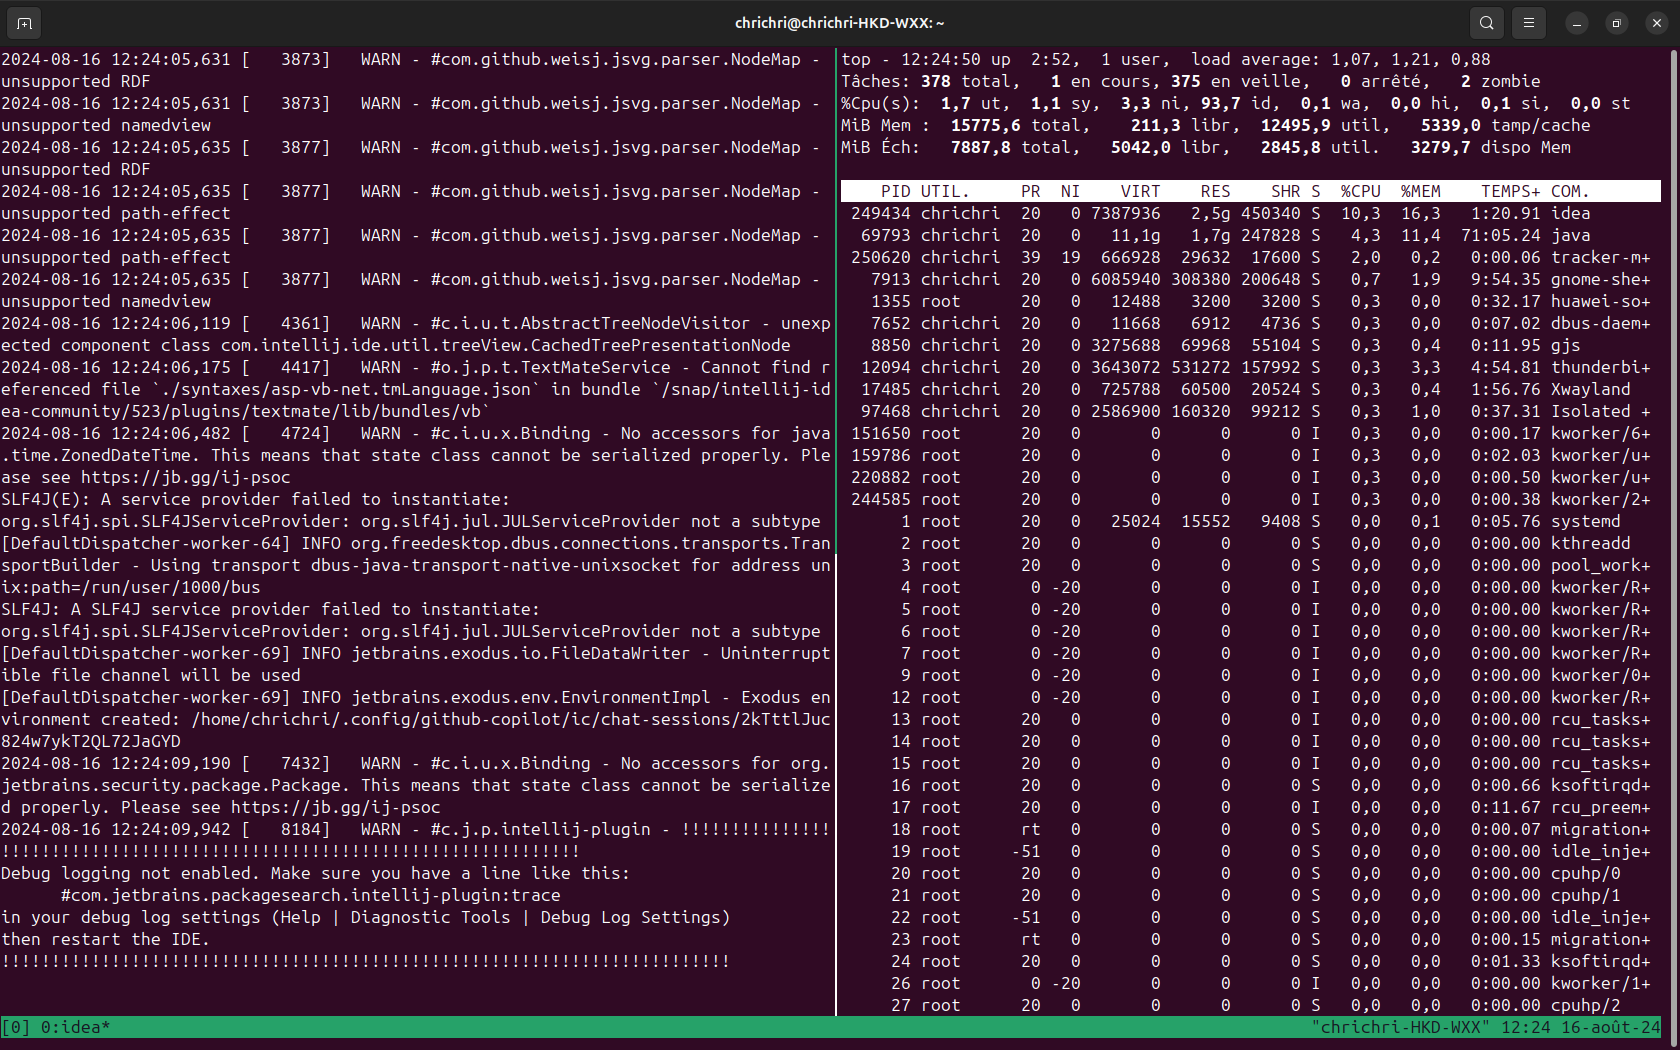
\includegraphics[width=10.3cm]{image/tmux-illustration}
    \end{frame}

    \begin{frame}[fragile]{Shell}{Gérer plusieurs commandes en parallèle avec \lstinline{nohup}}
        \lstinline{nohup} vient de NO Hang UP, c'est une commande qui permet de lancer une autre commande en arrière-plan sans qu'elle soit interrompue par la fermeture de la session Shell.
        Idéale donc pour les longs processus.
        L'output de la commande va par défault dans le fichier \lstinline{nohup.out}.
        \bigbreak
        Il suffit de préfixer la commande par \lstinline{nohup} et d'ajouter un \lstinline{&} pour libérer le terminal.
        \lstinline{nohup} indique le PID pour pouvoir stopper la commande au besoin et indique également quand la commande est terminée, si elle s'est arrêtée (Termine <code retour>) prématurément ou normalement (Fini).
        \begin{lstlisting}[language=bash]
$ nohup ls &
[1] 279343
nohup: les entrées sont ignorées et la sortie est ajoutée à 'nohup.out'
[1]+  Fini                    nohup ls
$ tail -n 3 nohup.out
technip
Téléchargements
ts-test
        \end{lstlisting}
    \end{frame}

    \begin{frame}{Shell}{Secure SHell (SSH)}
        La machine Linux à administrer sera le plus souvent dans un cloud, une salle serveur, un data center, elle sera distante.
        Dans une infrastructure sécurisée.
        \bigbreak
        Mais avec un user, un Shell par défaut, et un protocole sécurisé comme le SSH, nous allons pouvoir nous connecter et l'administrer à distance.
        \bigbreak
        Les bonnes pratiques sont d'utiliser les clés SSH uniquement, pas de connexion SSH avec l'utilisateur root,
        tutoriel utile~:
        \begin{itemize}
            \item \href{https://phoenixnap.com/kb/generate-setup-ssh-key-ubuntu}{Configuration du login SSH sur Ubuntu}
        \end{itemize}
        \bigbreak
        \centering
        
\includegraphics[width=3cm]{image/guy-in-front-of-desktop}
    \end{frame}

    \begin{frame}{Shell}{Sécurisation du SSH avec la cryptographie asymétrique}
        \begin{small}
            Pourquoi est-ce plus sécure d'utiliser une clé SSH plutôt qu'un mot de passe~?
            \bigbreak
            Quels algorithmes et taille de clés sont recommandés~?
            \pause
            \bigbreak
            Sur le site \url{https://jadaptive.com/ssh-key-management/the-benefits-of-ssh-key-authentication/} on trouve~:
            \begin{columns}
                \begin{column}{0.6\textwidth}
                    \begin{itemize}
                        \item Le mot de passe doit être communiqué à chaque connexion, il est donc plus vulnérable à une interception/sniffing/MITHM~.
                        La clé privée reste sur le client, elle n'est pas communiquée.
                        \item La clé SSH est plus complexe à deviner qu'un mot de passe.
                        \item On peut automatiser des taches depuis la machine cliente avec la clé SSH~.
                    \end{itemize}
                \end{column}
                \begin{column}{0.4\textwidth}
                    \centering
                    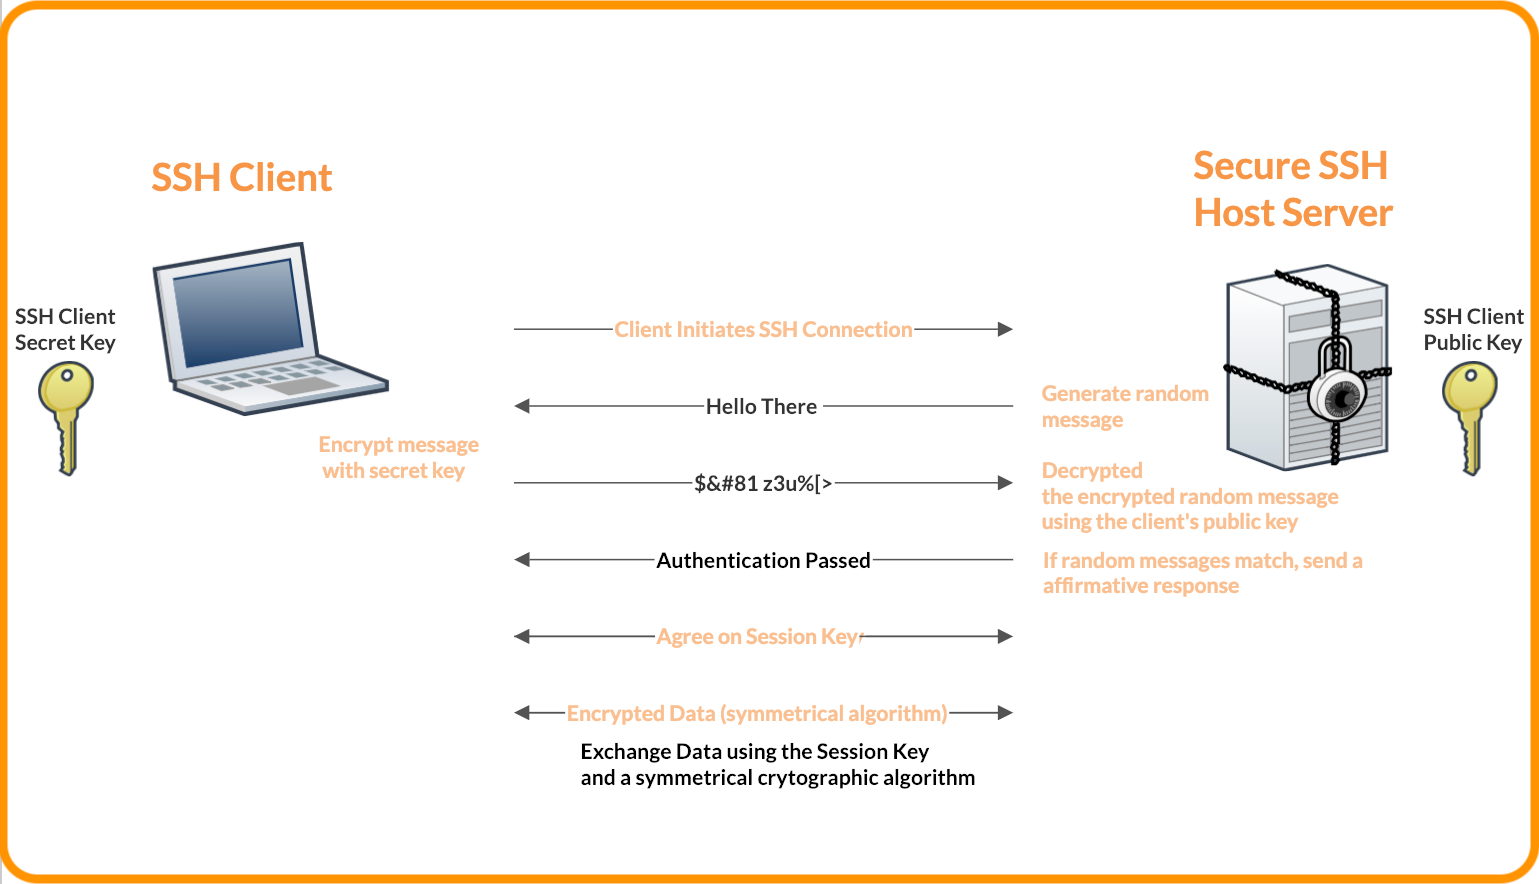
\includegraphics[width=5cm]{image/ssh-key-diagram} \\ Foxpass\footnotemark \\
                \end{column}
            \end{columns}
        \end{small}
    \end{frame}

    \begin{frame}{Shell}{Sécurisation du SSH avec la cryptographie asymétrique}
        Exercice \execcounterdispinc{}~:
        Restreindre l'accès à la VM au SSH avec une clé SSH, aucun mot de passe.
        \bigbreak
        Exercice \execcounterdispinc{}~:
        Créez un user pour un de vos camarades.
        Lui donner un Shell \lstinline{sh} par défaut.
        Configurez lui les clés SSH pour qu'il puisse se connecter.
    \end{frame}

    \begin{frame}[fragile]{Shell}{Une des solutions (commande à exécuter sur la VM)}
        Commande pour configurer la VM~:
        \begin{lstlisting}[language=bash][fragile]
# Configure SSH
sudo sed -i 's/PermitRootLogin yes/PermitRootLogin no/' /etc/ssh/sshd_config
sudo sed -i 's/PasswordAuthentication yes/PasswordAuthentication no/' /etc/ssh/sshd_config
# Restart SSH with the new configuration
sudo systemctl restart sshd
# Create the .ssh directory and the authorized_keys file
mkdir -p ~/.ssh
touch ~/.ssh/authorized_keys
# Add the public key to the authorized_keys file
echo "ssh-rsa AAAAB3NzaC1yc2EAAAADAQABAAABgQDQ8z4... chrichri@localhost" >> ~/.ssh/authorized_keys
        \end{lstlisting}
        \begin{center}
            
\includegraphics[width=2cm]{image/digicomp-lightbulb} \\ Expliquer chaque commande \\
        \end{center}
    \end{frame}

    \begin{frame}[fragile]{Shell}{Exemple de sécurisation des clés et des secrets sous Linux}
        Par défaut, Ubuntu desktop s’installe sur une partition non
        chiffrée (encrypter, ce n’est pas français on dit chiffrer~!~).
        Tout document peut donc être lu avec un disque de
        démarrage (live CD, USB bootable, \textit{etc}) ou si le disque dur
        est extrait et lu (vol, perte du desktop\ldots).
        \bigbreak
        Avec le package \lstinline{ecryptfs-utils} on peut chiffrer une partition~:
        \begin{lstlisting}[language=bash]
$ sudo apt-get install ecryptfs-utils
$ ecryptfs-setup-private
$ cp -r .ssh/ Private/ # Pour proteger les clés SSH on les déplace
$ ln -s /home/<mon user Ubuntu>/Private/.ssh/ . # Lien symbolique
        \end{lstlisting}
        Output~:
        \begin{lstlisting}
$ ls ~/.ssh -d -lha
lrwxrwxrwx 1 chrichri chrichri 28 janv. 14 21:27 /home/chrichri/.ssh -> /home/chrichri/Private/.ssh/
        \end{lstlisting}
        Il utilise le mot de passe de la session pour chiffrer/déchiffrer.
        Si la session n'est pas ouverte, les données sont chiffrées.
    \end{frame}

    \subsection{Commandes de base}\label{subsec:commandes-de-base}

    \begin{frame}{Commandes de base}{Commandes de base}
        \begin{itemize}
            \item \lstinline{ls}~: Liste les fichiers et répertoires.
            \item \lstinline{cd}~: Change de répertoire.
            \item \lstinline{pwd}~: Affiche le répertoire courant.
            \item \lstinline{cp}~: Copie des fichiers et des répertoires.
            \item \lstinline{mv}~: Déplace des fichiers et des répertoires.
            \item \lstinline{rm}~: Supprime des fichiers et des répertoires.
            \item \lstinline{mkdir}~: Crée des répertoires.
            \item \lstinline{cat}~: Affiche le contenu d'un fichier.
            \item \lstinline{head}~: Affiche les premières lignes d'un fichier.
            \item \lstinline{tail}~: Affiche les dernières lignes d'un fichier.
            \item \lstinline{touch}~: Crée un fichier vide.
            \item \lstinline{echo}~: Affiche une chaîne de caractères.
            \item \lstinline{du}~: Affiche l'espace disque utilisé par les fichiers.
            \item \lstinline{wget}~: Télécharge un fichier depuis URL~.
        \end{itemize}
    \end{frame}

    \begin{frame}[fragile]{Commandes de base}{Les options}
        Mais souvent, une commande seule ne suffit pas, il faut utiliser des options.

        Il existe deux solutions pour découvrir ces options~:
        \begin{itemize}
            \item Utiliser l'aide de la commande.
            Le plus souvent avec l'option \lstinline{--help} souvent équivalente à \lstinline{-h}.
            \begin{lstlisting}[language=bash]
$ ls --help # -h c'est human readable avec ls...
            \end{lstlisting}
            \item Une documentation souvent plus complète est accessible avec \lstinline{man}~:
            \begin{lstlisting}[language=bash]
$ man ls
            \end{lstlisting}
        \end{itemize}
    \end{frame}

    \begin{frame}[fragile]{Commandes de base}{Busy box}
        BusyBox est un logiciel libre qui fournit une implémentation unique d'environ 200 commandes UNIX standards dans un seul fichier pour diminuer la taille de ces derniers.
        Des distributions comme Alpine Linux l'utilisent pour réduire la taille de l'OS~.
        \begin{lstlisting}[language=bash,basicstyle=\tiny\ttfamily]
$ busybox
BusyBox v1.36.1 (Ubuntu 1:1.36.1-6ubuntu3) multi-call binary.
BusyBox is copyrighted by many authors between 1998-2015.
Licensed under GPLv2. See source distribution for detailed
copyright notices.

Usage: busybox [function [arguments]...]
or: busybox --list[-full]
or: busybox --install [-s] [DIR]
or: function [arguments]...

BusyBox is a multi-call binary that combines many common Unix
utilities into a single executable.  The shell in this build
is configured to run built-in utilities without $PATH search.
You don't need to install a link to busybox for each utility.
To run external program, use full path (/sbin/ip instead of ip).

Currently defined functions:
[, [[, acpid, adjtimex, ar, arch, arp, arping, ascii, ash, awk, base64, basename, bc, blkdiscard, blockdev, brctl, bunzip2, busybox, bzcat, bzip2, cal, cat, chgrp, chmod, chown, chpasswd, chroot, chvt, clear, cmp, cp,
cpio, crc32, crond, crontab, cttyhack, cut, date, dc, dd, deallocvt, depmod, devmem, df, diff, dirname, dmesg, dnsdomainname, dos2unix, dpkg, dpkg-deb, du, dumpkmap, dumpleases, echo, ed,
        \end{lstlisting}
    \end{frame}
    \begin{frame}[fragile]{Commandes de base}{Busy box}
        \begin{lstlisting}[language=bash,basicstyle=\tiny\ttfamily]
egrep, env, expand, expr, factor,
fallocate, false, fatattr, fdisk, fgrep, find, findfs, fold, free, freeramdisk, fsfreeze, fstrim, ftpget, ftpput, getopt, getty, grep, groups, gunzip, gzip, halt, head, hexdump, hostid, hostname, httpd, hwclock, i2cdetect,
i2cdump, i2cget, i2cset, i2ctransfer, id, ifconfig, ifdown, ifup, init, insmod, ionice, ip, ipcalc, kill, killall, klogd, last, less, link, linux32, linux64, linuxrc, ln, loadfont, loadkmap, logger, login, logname,
logread, losetup, ls, lsmod, lsscsi, lzcat, lzma, lzop, md5sum, mdev, microcom, mim, mkdir, mkdosfs, mke2fs, mkfifo, mknod, mkpasswd, mkswap, mktemp, modinfo, modprobe, more, mount, mt, mv, nameif, nbd-client, nc, netstat,
nl, nologin, nproc, nsenter, nslookup, nuke, od, openvt, partprobe, passwd, paste, patch, pidof, ping, ping6, pivot_root, poweroff, printf, ps, pwd, rdate, readlink, realpath, reboot, renice, reset, resume, rev, rm, rmdir,
rmmod, route, rpm, rpm2cpio, run-init, run-parts, sed, seq, setkeycodes, setpriv, setsid, sh, sha1sum, sha256sum, sha3sum, sha512sum, shred, shuf, sleep, sort, ssl_client, start-stop-daemon, stat, static-sh, strings, stty,
su, sulogin, svc, svok, swapoff, swapon, switch_root, sync, sysctl, syslogd, tac, tail, tar, taskset, tc, tee, telnet, telnetd, test, tftp, time, timeout, top, touch, tr, traceroute, traceroute6, true, truncate, ts, tty,
tunctl, ubirename, udhcpc, udhcpc6, udhcpd, uevent, umount, uname, uncompress, unexpand, uniq, unix2dos, unlink, unlzma, unshare, unxz, unzip, uptime, usleep, uudecode, uuencode, vconfig, vi, w, watch, watchdog, wc, wget,
which, who, whoami, xargs, xxd, xz, xzcat, yes, zcat
$ busybox ls
LICENSE            checkmytex.sh      compress-image.sh  dept.csv           employee.csv       sqlite-hr.sh       venv
        \end{lstlisting}
        Il s'utilise en préfixant la commande par \lstinline{busybox <commande>}.
        \begin{lstlisting}[language=bash,basicstyle=\tiny\ttfamily]
$ busybox sha256sum employee.csv
c148c36111463e962f490742af787c1f8e49776f09d89e19f71c6cdcf220240d  employee.csv
        \end{lstlisting}
    \end{frame}

    \begin{frame}{Commandes de base}{Commandes de base}{Exercice \execcounterdispinc{}~:}
        Le but est de préparer la configuration d'un nouveau service après avoir sauvegardé l'original.
        \begin{itemize}
            \item Créer un répertoire de backup des services dans votre \textquote{home} nommé \lstinline{service-backup}.
            \item Se déplacer dans le répertoire des services \lstinline{/etc/systemd/system}.
            \item Copier un service dans \lstinline{service-backup}.
            \item Afficher le contenu du fichier copié pour vérifier ce dernier.
            \item Créer un répertoire de développement des services dans votre \textquote{home} nommé \lstinline{service-dev}.
            \item Copier le contenu de \lstinline{service-backup} dans \lstinline{service-dev}.
            \item Modifier la description du service de \lstinline{service-dev} avec un éditeur et sauvegarder.
        \end{itemize}
    \end{frame}

    \begin{frame}{Commandes de base}{Opérateurs de redirection et piping\footnote{Five ways to use redirect operators in Bash, \url{https://www.redhat.com/sysadmin/redirect-operators-bash}}}
        \begin{footnotesize}
            \begin{itemize}
                \item \lstinline{>}~: Redirige la sortie standard vers un fichier.
                \item \lstinline{>>}~: Redirige la sortie standard vers un fichier en ajoutant le contenu à la fin.
                \item \lstinline{<}~: Redirige un fichier vers l'entrée standard.
                \item \lstinline{2>}~: Redirige la sortie d'erreur vers un fichier.
                \item \lstinline{&>}~: Redirige la sortie standard et d'erreur vers un fichier.
                \item \lstinline{|}~: Piping, redirige la sortie standard d'une commande vers l'entrée standard d'une autre.
            \end{itemize}
            À quoi ces opérateurs peuvent-ils servir~?
            \begin{center}
                
\includegraphics[width=3cm]{image/question-mark}
            \end{center}
        \end{footnotesize}
    \end{frame}

    \begin{frame}{Commandes de base}{Opérateurs logiques}
        \begin{itemize}
            \item \lstinline{||}~: Exécute la commande suivante si la précédente a échoué.
            \item \lstinline{\&\&}~: Exécute la commande suivante si la précédente a réussi.
        \end{itemize}
        Ils peuvent définir le comportement d'un script et être utilisés dans des conditions.
        \bigbreak
        Lancer un \lstinline{sudo apt upgrade} uniquement si \lstinline{sudo apt update} \textbf{a fonctionné}.
        \bigbreak
        Logger un message d'erreur si \lstinline{ls klazkjhfzklefjh} \textbf{n'a pas fonctionné}.
        \bigbreak
        \centering
        
\includegraphics[width=3cm]{image/guy-in-front-of-desktop}
    \end{frame}

    \begin{frame}{Commandes de base}{Les flux standards dans le Shell Linux\footnote{\label{standard-stream}The Standard Streams, \url{https://zedas.fr/posts/linux-explained-6-standard-streams/}}}
        \begin{itemize}
            \item \textbf{Les flux standards}~: Canaux de communication d'entrée et de sortie dans le shell.
            \item \textbf{entrée standard (Entrée standard)}~:
            \begin{itemize}
                \item Flux pour les données d'entrée d'un programme.
                \item Exemple~: Taper la commande \lstinline{echo "Coucou" | at now}, elle utilise l'entrée standard de la commande \lstinline{at}.
            \end{itemize}
            \item \textbf{sortie standard (Sortie standard)~:}
            \begin{itemize}
                \item Flux pour les données de sortie d'un programme.
                \item Exemple~: La sortie de \lstinline{ls} est affichée via la sortie standard.
            \end{itemize}
        \end{itemize}
    \end{frame}

    \begin{frame}{Commandes de base}{Les flux standards dans le Shell Linux\cref{standard-stream}}
        \begin{itemize}
            \item \textbf{sortie d'erreur (Erreur standard)}~:
            \begin{itemize}
                \item Flux pour les messages d'erreur ou diagnostics.
                \item Exemple~: L'erreur \lstinline{No such file or directory} de \lstinline{ls} est affichée via sortie d'erreur.
            \end{itemize}
            \item \textbf{Identifiants des flux~:}
            \begin{itemize}
                \item \textbf{0~:} entrée standard (stdin)
                \item \textbf{1~:} sortie standard (stdout)
                \item \textbf{2~:} sortie d'erreur (stderr)
            \end{itemize}
        \end{itemize}
    \end{frame}

    \begin{frame}{Commandes de base}{Les flux standards dans le Shell Linux\cref{standard-stream}}
        \centering
        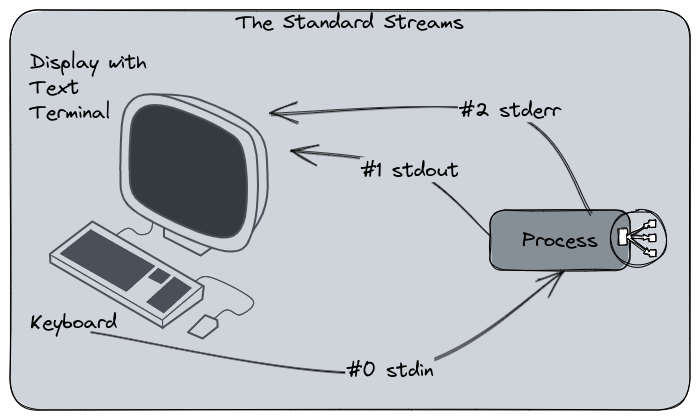
\includegraphics[width=10cm]{image/standard-stream-computer}
    \end{frame}

    \begin{frame}{Commandes de base}{Les flux standards dans le Shell Linux\cref{standard-stream}}
        \centering
        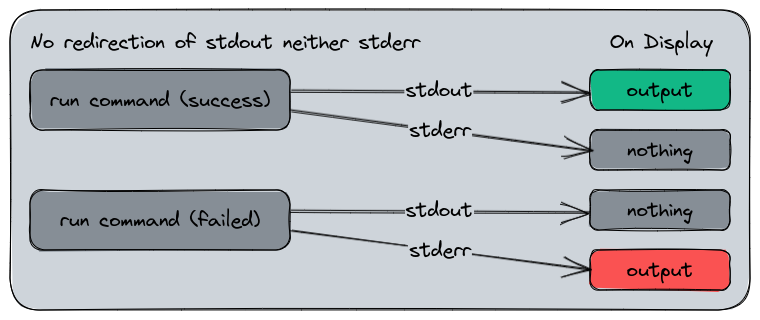
\includegraphics[width=10cm]{image/shell-stream-no-redirect}
    \end{frame}

    \begin{frame}{Commandes de base}{Exercice \execcounterdispinc{}~:}
        Le but est de créer un fichier source d'un script Shell en y ajoutant ligne par ligne les commandes~:
        \begin{itemize}
            \item Initier la création d'un script Shell nommé \lstinline{discover.sh} dans votre \textquote{home} avec un commentaire (chaîne de caractères préfixée par \lstinline{\#}) descriptif.
            \item Afficher un message indiquant que le \textquote{current working directory} va s'afficher.
            \item Afficher le current working directory.
            \item Afficher un message indiquant que les fichiers et répertoires du répertoire courant vont s'afficher.
            \item Afficher la liste des fichiers et répertoires du répertoire courant.
        \end{itemize}

        Inutile donc indispensable~:
        \begin{itemize}
            \item Changer de répertoire pour aller dans le répertoire courant avec le pipe.
        \end{itemize}
    \end{frame}

    \begin{frame}{Commandes de base}{Exercice \execcounterdispinc{}~:}
        \begin{itemize}
            \item Rediriger la sortie standard de la commande \lstinline{ls} dans un fichier \lstinline{ls-output.txt}.
            \item Rediriger la sortie d'erreur de la commande \lstinline{ls} dans un fichier \lstinline{ls-error.txt}.
            \item Rediriger les deux flux dans un fichier \lstinline{ls-output-error.txt}.
            \item Rediriger le contenu du fichier \lstinline{ls-output.txt} dans l'entrée standard de la commande \lstinline{grep} pour filter sur un type d'extension de fichier.
        \end{itemize}
    \end{frame}

    \subsection{Arguments et extensions des noms de fichiers}\label{subsec:arguments-extension}


    \begin{frame}{Syntaxe Shell}{Variables et Arguments\footnote{\label{devhint-bash}Bash scripting cheatsheet, \url{https://devhints.io/bash}}}
        \bigbreak
        \begin{itemize}
            \item Définir une variable~: \lstinline{NOM=valeur}
            \item Définir une constante~: \lstinline{readonly NOM=valeur}
            \item Référencer~: \lstinline{$NOM}
            \item Paramètres spéciaux~:
            \begin{itemize}
                \item \lstinline{$\#} - Nombre d'arguments
                \item \lstinline{$@} - Tous les arguments positionnels comme chaînes séparées
                \item \lstinline{$*} - Tous les arguments positionnels comme une seule chaîne
                \item \lstinline{$1}, \lstinline{$2}, \textit{etc} - Arguments positionnels
                \item \lstinline{$_} - Dernier argument du dernier processus
            \end{itemize}
        \end{itemize}
    \end{frame}

    \begin{frame}[fragile]{Syntaxe Shell}{Extension des noms de fichiers des scripts Shell}
        Ils peuvent tous avoir avoir l'extension \lstinline{.sh} quelque soit le type de Shell.
        \bigbreak
        Mais il peut être pratique de les différencier surtout lorsqu'ils sont spécifiques à un interpréteur Shell.
        On les différencie avec en extension leur nom ou diminutif de Shell, \lstinline{sh} pour le POSIX, \lstinline{ksh} pour me Korn, \lstinline{bash} pour le Bash, \lstinline{zsh} pour le Z Shell, \lstinline{csh} pour le C Shell, \textit{etc}.
        \bigbreak
        Exemple ici pour différencier Bash de Korn~:
        \begin{lstlisting}[language=bash]
$ ls -lha | grep fibo_cached.*sh
-rw-rw-r-- 1 chrichri chrichri  449 août  27 23:48 fibo_cached.bash
-rw-rw-r-- 1 chrichri chrichri  461 août  27 23:44 fibo_cached.ksh
-rw-rw-r-- 1 chrichri chrichri  554 août  28 12:15 fibo.sh
        \end{lstlisting}
    \end{frame}

    \begin{frame}[fragile]{Syntaxe Shell}{La compatibilité}
        Si on tente d'utiliser les syntaxes Bash, Korn et POSIX avec les autres interpréteurs~:
        \begin{lstlisting}[language=bash,basicstyle=\tiny\ttfamily]
$ bash fibo_cached.bash 10
55
$ bash fibo.sh 10
55
$ bash fibo_cached.ksh 10
55
$ ksh fibo_cached.bash 10
fibo_cached.bash[3]: declare: not found
fibo_cached.bash[26]: fibo_cached[6]: local: not found

$ ksh fibo_cached.ksh 10
55
$ ksh fibo.sh 10
55
$ sh fibo_cached.bash 10
fibo_cached.bash: 3: declare: not found
fibo_cached.bash: 7: cannot open 2: No such file
fibo_cached.bash: 12: Bad substitution
$ sh fibo_cached.ksh 10
fibo_cached.ksh: 3: typeset: not found
fibo_cached.ksh: 6: typeset: not found
fibo_cached.ksh: 7: cannot open 2: No such file
fibo_cached.ksh: 12: Bad substitution
$ sh fibo.sh 10
55
        \end{lstlisting}
    \end{frame}

    \begin{frame}{Syntaxe Shell}{La compatibilité}
        \begin{footnotesize}
            \begin{table}[ht]
                \begin{tabular}{|p{2.5cm}|p{2.5cm}|p{2.5cm}|p{2.5cm}|}
                    \hline
                    \textbf{Script}               & \textbf{Interpréteur bash} & \textbf{Interpréteur ksh}                                  & \textbf{Interpréteur sh}                                                          \\ \hline
                    \lstinline{fibo\_cached.bash} & \emoji{check-mark-button}  & \emoji{no-entry} \lstinline{declare et local introuvables} & \emoji{no-entry} \lstinline{declare, cannot open 2, Bad substitution} \\ \hline
                    \lstinline{fibo\_cached.ksh}  & \emoji{check-mark-button}  & \emoji{check-mark-button}                                                       & \emoji{no-entry} \lstinline{typeset introuvable, cannot open 2, Bad substitution} \\ \hline
                    \lstinline{fibo\_cached.sh}   & \emoji{check-mark-button}  & \emoji{check-mark-button}                                  & \emoji{check-mark-button}                                                         \\ \hline
                \end{tabular}
                \caption{Matrice de compatibilité entre les interpréteurs de Shell et les syntaxes}
            \end{table}
        \end{footnotesize}
    \end{frame}

    \subsection{Variables prédéfinies}\label{subsec:variables-predefinies}

    \begin{frame}[fragile]{Variables prédéfinies}{Lister les variables d'environnment}
        \begin{footnotesize}
            Les variables d'environnement sont des variables qui sont définies pour le Shell et les processus qui s'exécutent dans ce Shell.
            On peut donc les utiliser dans le terminal ou un script.
            \bigbreak
            Pour les lister, on utilise la commande \lstinline{printenv}.
            On y trouve entre autre le Shell en cours d'utilisation \lstinline{SHELL}, le \lstinline{PATH}, le \lstinline{HOME}, le \lstinline{USER}, \textit{etc}
            \begin{lstlisting}[language=bash,basicstyle=\tiny\ttfamily]
# Display des variables d'environnement
$ printenv | grep USER=
USER=chrichri
$ printenv | grep SHELL=
SHELL=/usr/bin/bash
$ printenv | grep HOME=
HOME=/home/chrichri
$ printenv | grep ^PATH=
PATH=/home/chrichri/anaconda3/bin:/home/chrichri/.opam/default/bin:/home/chrichri/.cargo/bin:/home/chrichri/.local/bin:/usr/local/sbin:/usr/local/bin:/usr/sbin:/usr/bin:/sbin:/bin:/usr/games:/usr/local/games:/snap/bin:/snap/bin:/home/chrichri/.dotnet/tools
# Usage des variables d'environnement, comme tout autre variable
$ echo "Qui suis-je: ${USER}"
Qui suis-je: chrichri
            \end{lstlisting}
            Des explications plus exhaustives sur chaque variable d'environnement sont en ligne\footnote{Linux List All Environment Variables Command, \url{https://www.cyberciti.biz/faq/linux-list-all-environment-variables-env-command/}}.
        \end{footnotesize}
    \end{frame}

    \subsection{Les alias}\label{subsec:alias}

    \begin{frame}[fragile]{Shell}{Les alias}
        Les alias sont des raccourcis pour des commandes.
        Ils sont donc intéressants à paramétrer pour les commandes longues et récurrentes.
        \bigbreak
        Par exemple, pour la commande \lstinline{ls -l}~:
        \begin{lstlisting}[language=bash]
$ alias ll='ls -l'
$ ll
total 3484
-rw-rw-r-- 1 chrichri chrichri     249 août  15 12:35 analytic-using-awk.sh
-rw-rw-r-- 1 chrichri chrichri      82 août  10 23:04 checkmytex.sh
...
        \end{lstlisting}
        \bigbreak
        Pour rendre l'alias permanent, il faut l'ajouter dans le fichier \lstinline{.bashrc} ou \lstinline{.bash_profile}~:
        \begin{lstlisting}[language=bash]
$ echo "alias ll='ls -l'" >> ~/.bashrc
        \end{lstlisting}
        De cette manière à chaque fois qu'un Shell est ouvert, la commande est exécutée.
    \end{frame}

    \subsection{Vous décidez~: les options}\label{subsec:shell-options}

    \begin{frame}[fragile]{Shell}{Vous décidez~: les options}
        On peut accéder aux options de Bash et Korn Shell avec l'option \lstinline{--help} qui liste dans le terminal les autres options.
        \bigbreak
        Sinon, comme pour toutes commandes, on peut accéder à la documentation avec \lstinline{man <nom de la commande>}.
        \bigbreak
        Exercice \execcounterdispinc~:
        \begin{itemize}
            \item Trouver l'option \lstinline{bash} pour lancer un script dans un environnement restreint, plus contrôlé que l'environnement standard.
            \item Lancer un script avec cette option.
        \end{itemize}
        Exercice \execcounterdispinc~:
        \begin{itemize}
            \item Trouver l'option \lstinline{sh} de debug.
            \item Lancer un script avec cette option.
        \end{itemize}
    \end{frame}

    \subsection{On récolte ce qu'on sème~: échos et variables}\label{subsec:recolte}

    \begin{frame}[fragile]{On récolte ce qu'on sème~: échos et variables}{l'\lstinline{echo} vs le \lstinline{return}}
        \begin{itemize}
            \item Définir une fonction~:
            \begin{lstlisting}[language=bash,basicstyle=\ttfamily\tiny]
mafunc() {
    echo "Bonjour $1"
}
            \end{lstlisting}
            \lstinline{$1} est le premier argument passé à la fonction.
            \item Retourner des valeurs avec \lstinline{echo}~:
            \begin{lstlisting}[language=bash,basicstyle=\ttfamily\tiny]
$ echo $(mafunc "Jean")
Bonjour Jean
            \end{lstlisting}
            \item Gestion des erreurs~:
            \begin{lstlisting}[language=bash,basicstyle=\ttfamily\tiny]
mafunc() {
    return 1
}
if mafunc; then
    echo "Succès"
else
    echo "Échec"
fi
Échec
            \end{lstlisting}
            \lstinline{return} est utilisé pour retourner un code retour mais aucune autre valeur.
            Il est compris entre 0 et 255.
        \end{itemize}
    \end{frame}

    \begin{frame}[fragile]{Variables prédéfinies}{Lister les variables d'environnment}
        Les variables d'environnement sont des variables qui sont définies pour le Shell et les processus qui s'exécutent dans ce Shell.
        On peut donc les utiliser dans le terminal ou un script.
        \bigbreak
        Pour les lister, on utilise la commande \lstinline{printenv}.
        On y trouve entre autre le Shell en cours d'utilisation \lstinline{SHELL}, le \lstinline{PATH}, le \lstinline{HOME}, le \lstinline{USER}, \textit{etc}
        \begin{lstlisting}[language=bash,basicstyle=\tiny\ttfamily]
# Display des variables d'environnement
$ printenv | grep USER=
USER=chrichri
$ printenv | grep SHELL=
SHELL=/usr/bin/bash
$ printenv | grep HOME=
HOME=/home/chrichri
$ printenv | grep ^PATH=
PATH=/home/chrichri/anaconda3/bin:/home/chrichri/.opam/default/bin:/home/chrichri/.cargo/bin:/home/chrichri/.local/bin:/usr/local/sbin:/usr/local/bin:/usr/sbin:/usr/bin:/sbin:/bin:/usr/games:/usr/local/games:/snap/bin:/snap/bin:/home/chrichri/.dotnet/tools
# Usage des variables d'environnement, comme tout autre variable
$ echo "Qui suis-je: ${USER}"
Qui suis-je: chrichri
        \end{lstlisting}
    \end{frame}


    \section{Aide}\label{sec:aide}

    \subsection{Où et quoi chercher~?}\label{subsec:aide-ou-quand}

    \begin{frame}{Où et quoi chercher~?}{En ligne}
        \begin{footnotesize}
            Les ressources~:
            \begin{itemize}
                \item \href{https://doc.ubuntu-fr.org/}{Aide à l'utilisation du forum Ubuntu‑FR}, un wiki.
                \item \href{https://www.cyberciti.biz/}{nixCraft} des articles sur les technologies de l'écosystème Unix et Linux.
                \item \href{https://www.redhat.com/}{RedHat} des articles sur les technologies de l'écosystème Linux de RedHat, une des principales distributions de type \textquote{entreprise}.
                Mais le contenu s'applique souvent à tous les Linux.
            \end{itemize}
            Les medias~:
            \begin{itemize}
                \item \href{http://www.youtube.com/@Computerphile}{Computerphile}, interview d'académiques de Nottingham Uni et d'experts du monde entier.
                \item \href{http://www.youtube.com/@IBMTechnology}{Chaine YouTube d'IBM, IBM Technology} format court par les experts d'IBM~.
            \end{itemize}
            Les forums~:
            \begin{itemize}
                \item \href{https://askubuntu.com/}{Ask Ubuntu} blog de la galaxy Stack Exchange Inc, Stack Overflow, \textit{etc}.
                \item \href{https://ubuntuforums.org}{Ubuntu forums} forum et ressources très populaire en anglais.
            \end{itemize}
        \end{footnotesize}
    \end{frame}

    \begin{frame}[fragile]{Où et quoi chercher~?}{Dans le terminal}
        Comme vue précédemment la principale aide ligne de commande est le \textquote{help} de la commande \lstinline{-h} ou \lstinline{--help}.

        Si ce dernier ne suffit pas \lstinline{man <commande à découvrir>} renvoie vers la documentation du package ou du logiciel qui est encore plus complète.
        \bigbreak
        Exercice \execcounterdispinc~:
        Enregistrer le code C suivant dans le fichier \lstinline{hello.c}~:
        \begin{lstlisting}[language=C]
#include<stdio.h>
int main()
{
  printf("\nHello world!");
  return 0;
}
        \end{lstlisting}
        Compiler le code avec \lstinline{gcc} de manière à produire un exécutable nommé \lstinline{hello}.
        \bigbreak
    \end{frame}

    \begin{frame}[fragile]{Où et quoi chercher~?}{Dans le terminal}
        Exercice \execcounterdispinc~:
        Lister les \textit{optimizations} possibles du compilateur \lstinline{gcc}.
        Et trouver celle permettant d'optimiser pour la place.
        \bigbreak
        \centering
        
\includegraphics[width=3cm]{image/guy-in-front-of-desktop}
        \pause
        \begin{lstlisting}[language=bash]
$ gcc --help=optimizers
The following options control optimizations:
  -O<number>                  Set optimization level to <number>.
  -Ofast                      Optimize for speed disregarding exact standards compliance.
  -Og                         Optimize for debugging experience rather than speed or size.
...
        \end{lstlisting}
    \end{frame}

    \begin{frame}[fragile]{Où et quoi chercher~?}{Dans le terminal}
        La commande \lstinline{apropos} équivalent à \lstinline{man -k} permet de chercher une commande avec la syntaxe \lstinline{apropos <pattern chaine ou RegExp>}~:
        \begin{lstlisting}[language=bash]
$ apropos ^gcc- # Exemple d'une RegExp
gcc-10 (1)           - GNU project C and C++ compiler
gcc-11 (1)           - GNU project C and C++ compiler
...
$ apropos riscv64-linux-gnu-gcc # Exemple d'une Chaine de caractère
riscv64-linux-gnu-gcc (1) - GNU project C and C++ compiler
riscv64-linux-gnu-gcc-13 (1) - GNU project C and C++ compiler
riscv64-linux-gnu-gcc-ar (1) - a wrapper around ar adding the --plugin option
riscv64-linux-gnu-gcc-ar-13 (1) - a wrapper around ar adding the --plugin option
riscv64-linux-gnu-gcc-nm (1) - a wrapper around nm adding the --plugin option
riscv64-linux-gnu-gcc-nm-13 (1) - a wrapper around nm adding the --plugin option
riscv64-linux-gnu-gcc-ranlib (1) - a wrapper around ranlib adding the --plugin option
riscv64-linux-gnu-gcc-ranlib-13 (1) - a wrapper around ranlib adding the --plugin option
        \end{lstlisting}
    \end{frame}

    \begin{frame}{Où et quoi chercher~?}{Dans les livres}
        \centering
        
\includegraphics[width=6cm]{image/lpi-book}
    \end{frame}

    \begin{frame}{Où et quoi chercher~?}{Dans les livres}
        Un \href{https://github.com/bobbyiliev/101-linux-commands-ebook?tab=readme-ov-file}{ebook gratuit sur GitHub} qui couvre les commandes Linux courantes.
        \bigbreak
        \centering
        
\includegraphics[width=6cm]{image/wise-tux}
    \end{frame}

    \begin{frame}{Où et quoi chercher~?}{Le GUI d'aide}
        \centering
        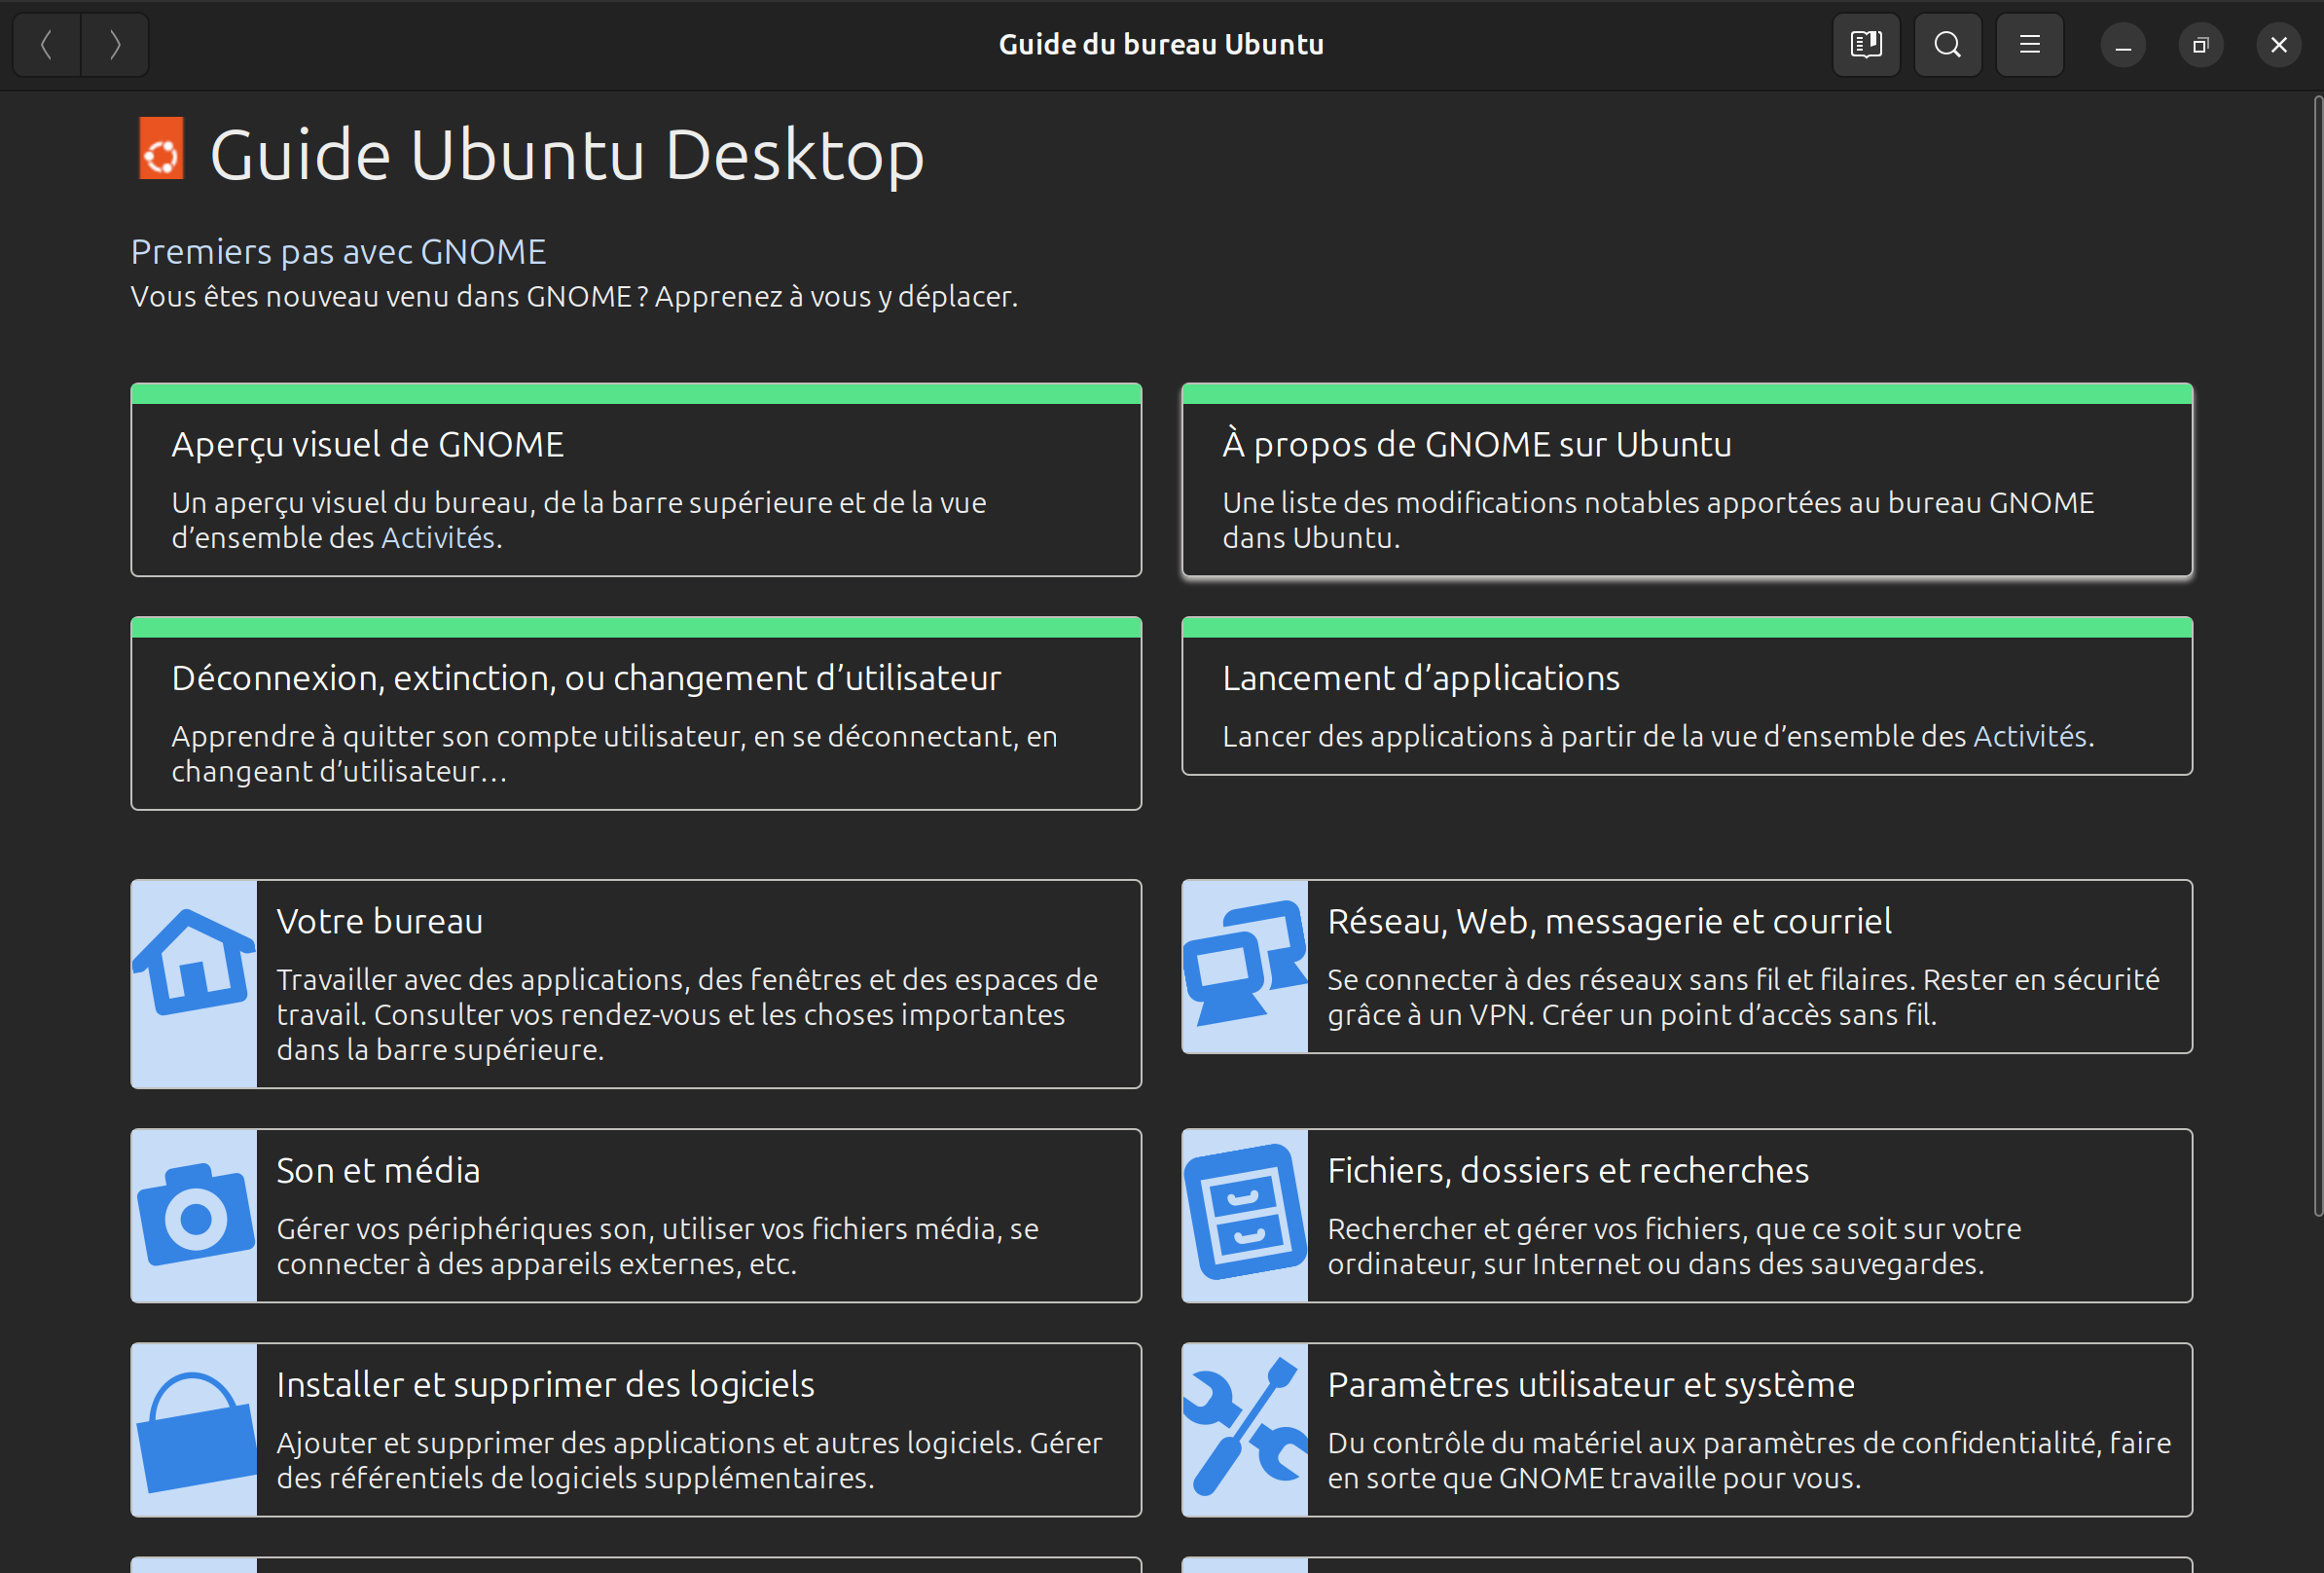
\includegraphics[width=10cm]{image/aide}
    \end{frame}

    \begin{frame}[fragile]{Où et quoi chercher~?}{Dans le terminal}
        \lstinline{whatis} permet de découvrir une commande avec la syntaxe \lstinline{whatis <pattern chaine ou RegExp>}.
        \bigbreak
        Par exemple avec cette commande de compression du fichier \lstinline{checkmytex.sh}~:
        \begin{lstlisting}[language=bash,basicstyle=\tiny\ttfamily]
$ whatis 7z a checkmytex.7z checkmytex.sh
7z (1)               - 7-Zip file archiver with a high compression ratio
a : rien d'adéquat
checkmytex.7z : rien d'adéquat
checkmytex.sh : rien d'adéquat
$ 7z a checkmytex.7z checkmytex.sh

7-Zip 23.01 (x64) : Copyright (c) 1999-2023 Igor Pavlov : 2023-06-20
 64-bit locale=fr_FR.UTF-8 Threads:8 OPEN_MAX:1048576

Scanning the drive:
1 file, 82 bytes (1 KiB)

Creating archive: checkmytex.7z

Add new data to archive: 1 file, 82 bytes (1 KiB)


Files read from disk: 1
Archive size: 210 bytes (1 KiB)
Everything is Ok
        \end{lstlisting}
    \end{frame}


    \section{Éditeurs}\label{sec:editor}

    \subsection{VS Code de Microsoft}\label{subsec:vscode}

    \begin{frame}{Editeurs}{VS Code de Microsoft}
        L'objectif de cette section est d'éditer un script Shell dans un environment dédié au développement.
        Un environment qui contient tous les outils nécessaires pour trouver rapidement les erreurs de syntaxe et tester son script.
        \bigbreak
        Pour le lancer taper \textquote{code} dans la barre de recherche de Linux ou \lstinline{code .} dans un terminal pour le lancer dans le répertoire courant.
        \begin{itemize}
            \item Ouvrir VS Code.
            \item Ouvrir ou créer le fichier contenant le code Shell.
            \item Trouver un plugin dédié au développement Shell dans la \textit{marketplace}.
            Ici \textquote{ShellCheck} pour la vérification de la syntaxe.
            En lisant la doc on comprend que c'est une intégration de ShellCheck qui vient sans ce dernier sur certaines plateformes.
            Il faut installer ShellCheck.
            \item Installer le plugin.
            \item Tester le plugin en écrivant sciemment un code erroné.
        \end{itemize}
    \end{frame}

    \begin{frame}{Editeurs}{VS Code de Microsoft}
        \centering
        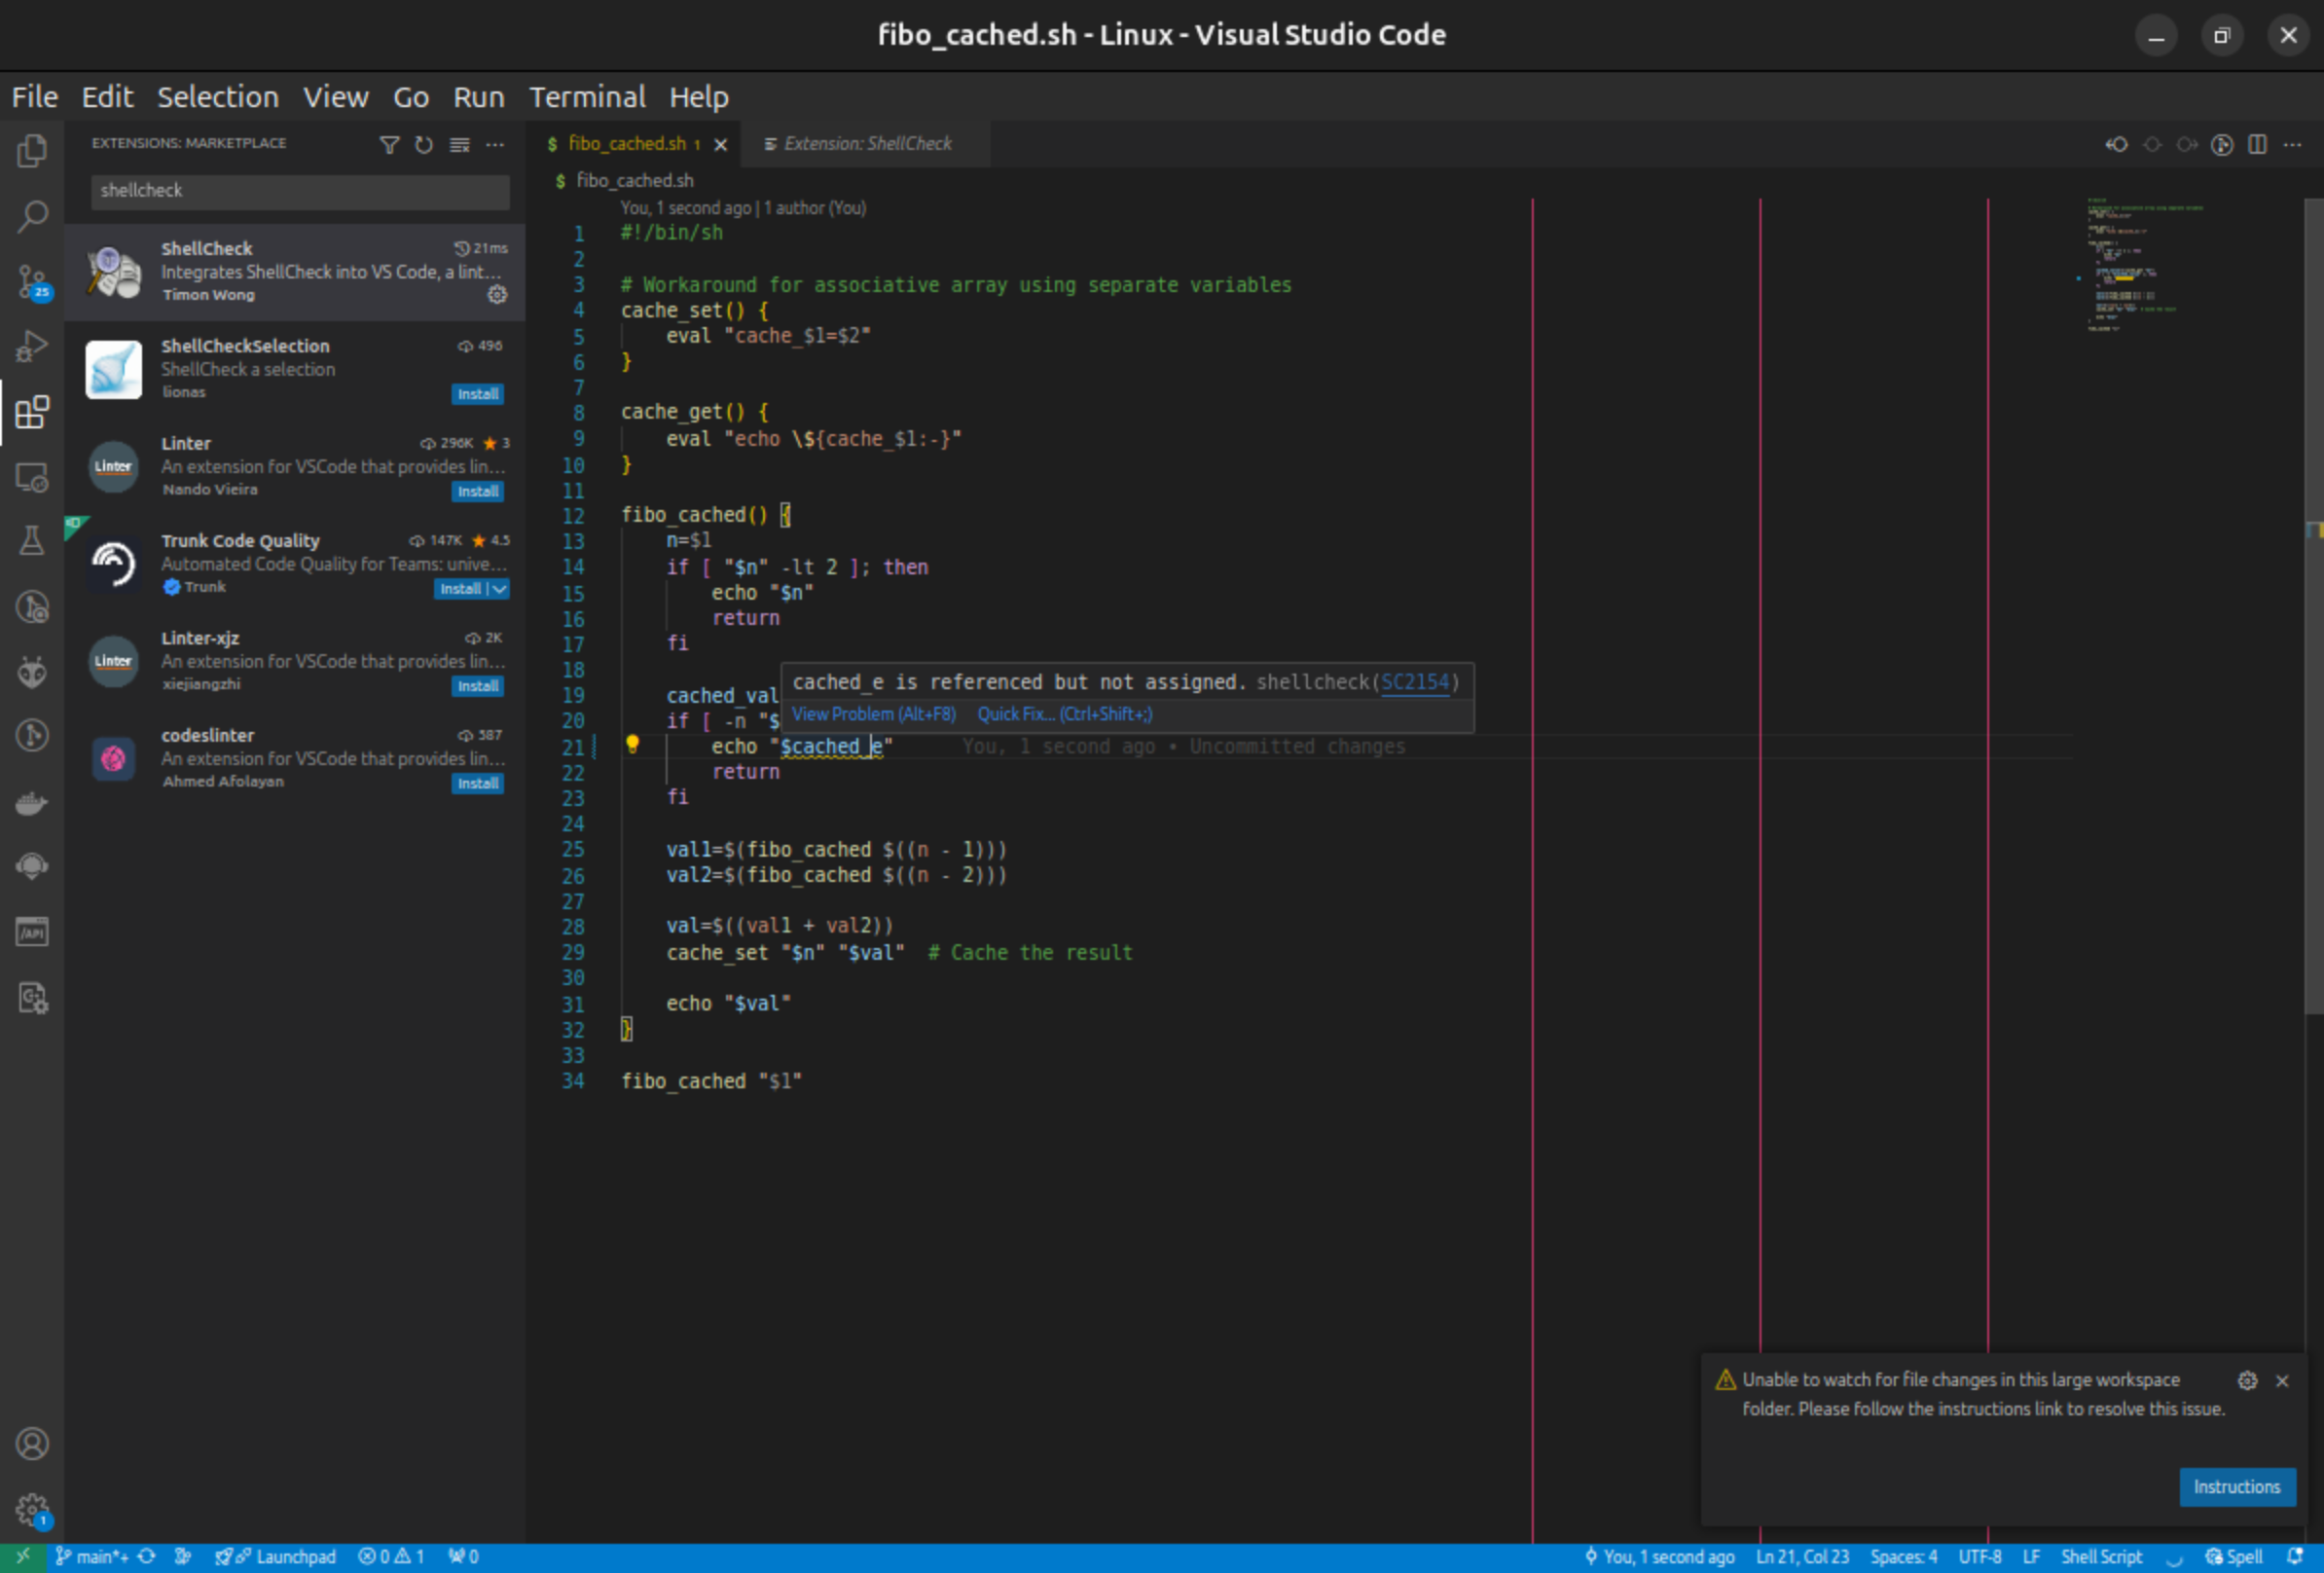
\includegraphics[width=11cm]{image/shellcheck-install}
    \end{frame}

    \begin{frame}[fragile]{Editeurs}{VS Code de Microsoft}
        Les erreurs/warning qui sont en ligne apparaissent dans l'IDE VS Code.
        \begin{lstlisting}[language=bash,basicstyle=\tiny\ttfamily]
$ shellcheck fibo.ksh

In fibo.ksh line 7:
        echo $n
             ^-- SC2086 (info): Double quote to prevent globbing and word splitting.

Did you mean:
        echo "$n"


In fibo.ksh line 11:
    typeset val1=$(fibo $((n - 1)))
            ^--^ SC2034 (warning): val1 appears unused. Verify use (or export if used externally).
            ^--^ SC2155 (warning): Declare and assign separately to avoid masking return values.


In fibo.ksh line 12:
    typeset val2=$(fibo $((n - 2)))
            ^--^ SC2034 (warning): val2 appears unused. Verify use (or export if used externally).
            ^--^ SC2155 (warning): Declare and assign separately to avoid masking return values.


In fibo.ksh line 14:
    typeset val=$((valeur1 + valeur2))
                   ^-----^ SC2154 (warning): valeur1 is referenced but not assigned.
                             ^-----^ SC2154 (warning): valeur2 is referenced but not assigned.
        \end{lstlisting}
    \end{frame}

    \begin{frame}{Editeurs}{VS Code de Microsoft}
        \centering
        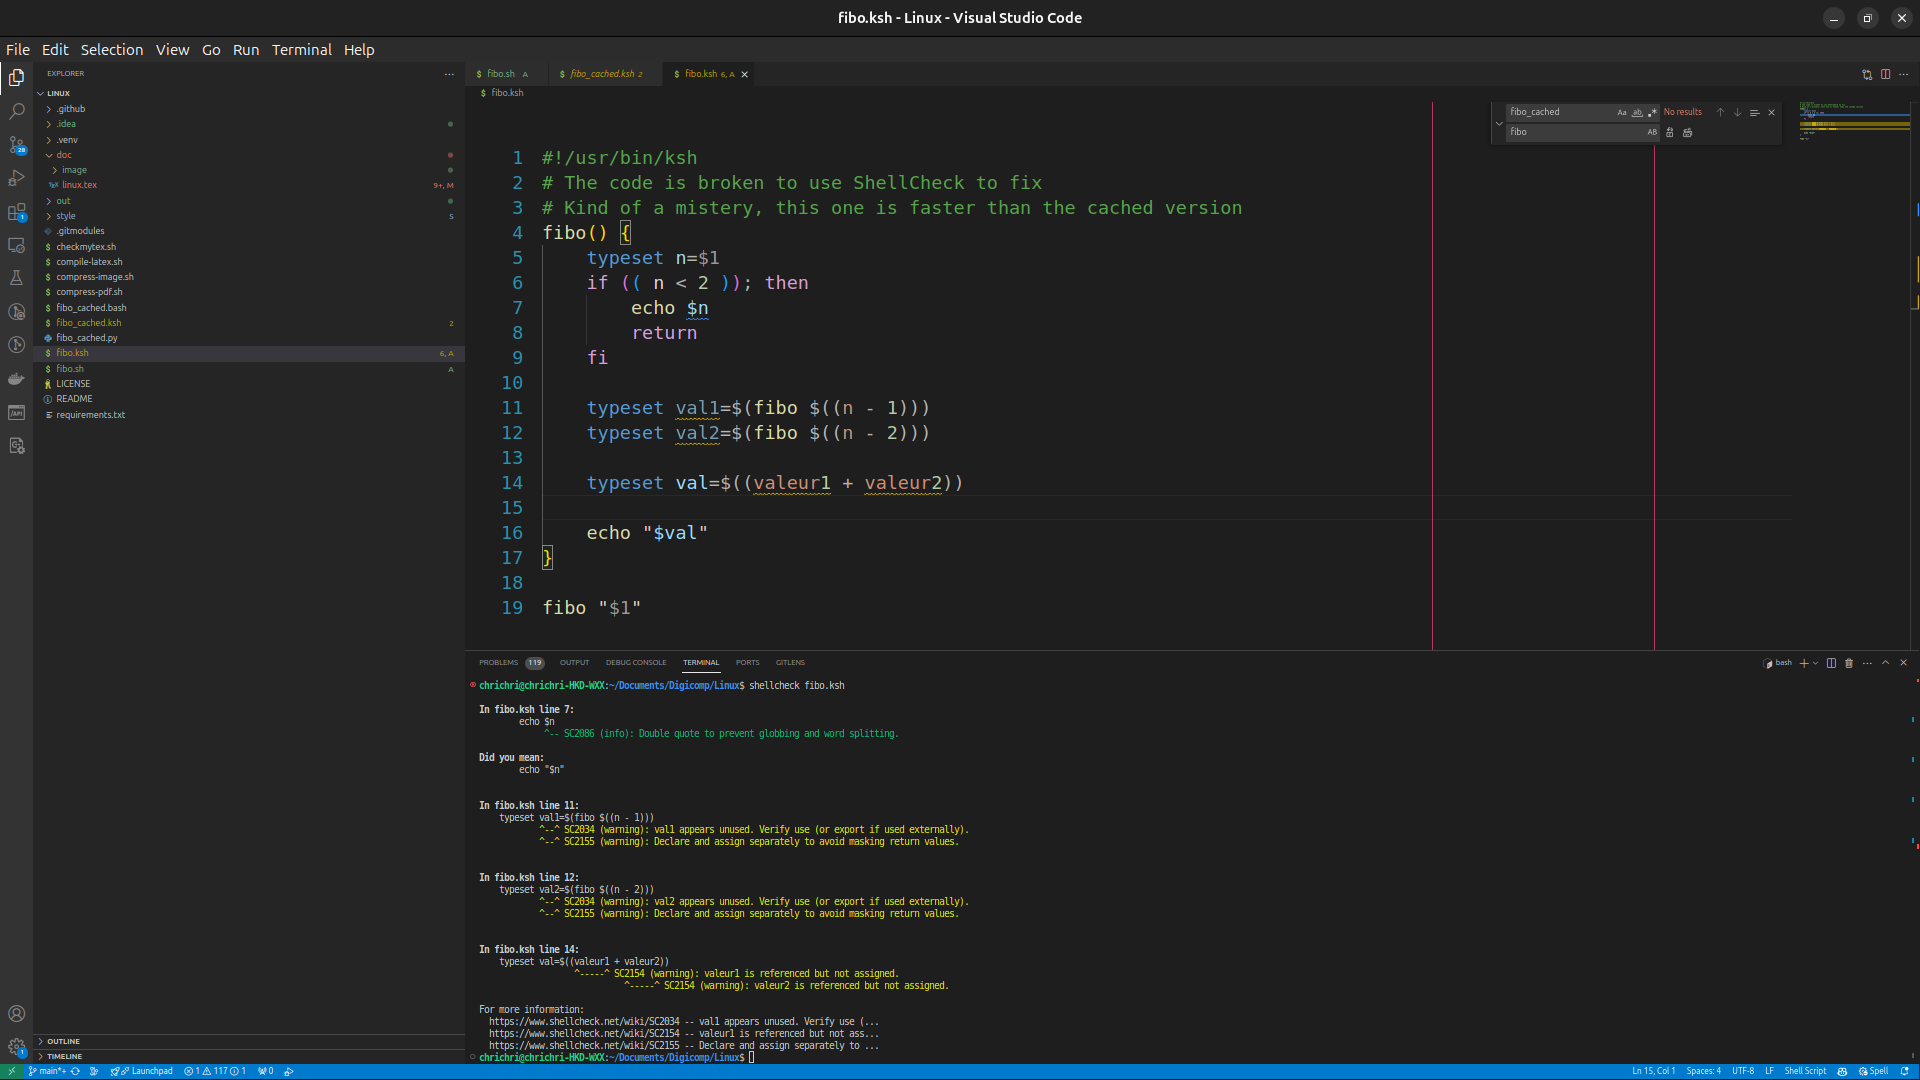
\includegraphics[width=12cm]{image/shellcheck-warning}
    \end{frame}

    \begin{frame}{Editeurs}{Exercice \execcounterdispinc}
        Cette exercice a pour but d'illustrer que les éditeurs fournissent une aide pour tout type de langage.
        \begin{itemize}
            \item Installer VS Code.
            \item Installer le plugin ShellCheck.
            \item Ouvrir un fichier le fichier \lstinline{fibo.sh} dans VS Code.
            \item Essayer de le lancer avec \lstinline{sh}.
            \item Corriger les erreurs et même les warnings mis en évidence par ShellCheck.
            \item Relancer le script pour vérifier qu'il fonctionne.
        \end{itemize}
        \bigbreak
        \centering
        \includegraphics[width=3cm]{image/question-mark}
    \end{frame}

    \begin{frame}{Editeurs}{Exercice \execcounterdispinc}
        De la même manière, cet IDE permet de modifier de configuration.
        Comme par les services configurés au format parfois appelé \textquote{Unit file}.
        \begin{itemize}
            \item Copier une configuration de service de \lstinline{/etc/systemd/system} dans le répertoire courant.
            \item Vérifier qu'il n'y pas de \textit{syntaxe highlighting}.
            \item Trouver un plugin pour le format \textquote{Unit file}.
            \item Installer le plugin.
            \item Vérifier que le formatage du fichier de configuration est bien pris en charge par le plugin installé.
        \end{itemize}
        \bigbreak
        \centering
        \includegraphics[width=3cm]{image/question-mark}
    \end{frame}


    \section{Files et Directories}\label{sec:files-directories}

    \begin{frame}[fragile]{Files et Directories}{Quel type de fichier~?}
        La liste des fichiers est trop longue pour qu'un registre soit tenu.
        Chacun peut créer son extension.
        Mais la commande \lstinline{file <chemin du fichier ou dossier>}, en examinant le contenu, nous indique le type de fichier/dossier.
        \begin{lstlisting}[language=bash]
$ file fibo.sh
fibo.sh: POSIX shell script, ASCII text executable
$ file out/linux.pdf
out/linux.pdf: PDF document, version 1.5
$ file venv/bin/python3
venv/bin/python3: symbolic link to python
$ file venv/bin/python
venv/bin/python: symbolic link to /usr/bin/python3.12
$ file /usr/bin/python3.12
/usr/bin/python3.12: ELF 64-bit LSB executable, x86-64, version 1 (SYSV), dynamically linked, interpreter /lib64/ld-linux-x86-64.so.2, BuildID[sha1]=ccd329aaf9256b96135a9e3f97cbf4c3829377e1, for GNU/Linux 3.2.0, stripped
$ file fibo_cached.py
fibo_cached.py: Python script, ASCII text executable
        \end{lstlisting}
    \end{frame}

    \begin{frame}[fragile]{Files et Directories}{Quel type de doonées}
        On peut stocker les données sous deux familles de fichiers~:
        \begin{itemize}
            \item Les fichiers textes comme par exemple~:
            \begin{itemize}
                \item Les CSV~.
                \item Les fichiers texte ou Markdown.
                \item les fichiers du web comme XML, HTML, JSON~.
                \item Certains fichiers de log.
            \end{itemize}
            \item Les fichiers binaires~:
            \begin{itemize}
                \item Les fichiers de données des BBD SQL, noSQL~.
                \item Les tableurs de type Excel.
                \item Certains fichiers de log.
                \item Le dump du traffic d'une interface réseau.
            \end{itemize}
        \end{itemize}
    \end{frame}

    \begin{frame}{Files et Directories}{Quel type de doonées}
        Toutes les commandes \lstinline{awk}, \lstinline{grep}, \lstinline{sed}, \lstinline{sort}, \textit{etc}, ne traitent que des fichiers textes.
        \bigbreak
        Quel est l'intérêt de traiter des fichiers binaires~?
        \bigbreak
        \centering
        \includegraphics[width=3cm]{image/question-mark}
    \end{frame}

    \begin{frame}[fragile]{Commandes de traitement de données}{Variantes de ces outils}
        Dans les exemples précédents, nous n'avons manipulé que des données issues de fichier texte.
        Les données numériques prennent moins de place en binaire.
        \begin{lstlisting}[language=python]
from sys import getsizeof
from struct import pack
print("lentgh of the string:", getsizeof("65535"))
print("lentgh of the struct:", getsizeof(pack(">H", 0xffff)))
lentgh of the string: 46
lentgh of the struct: 35
        \end{lstlisting}
        La valeur d'un octet est comprise entre 0 et 255, mais pour obtenir du texte, on passe par une table de correspondance, un encodage, qui donnera un seul caractère.
        La valeur numérique la plus élevée pour ce même octet en texte est donc 9.
        \bigbreak
        Pour des soucis de performance, de coût (du cloud), il n'est pas rare que les formats de données soit binaires.
    \end{frame}

    \begin{frame}{Commandes de traitement de données}{Arborescence Linux\footnote{\label{arborescence-linux}Arborescence des répertoires d’Ubuntu, \url{https://doc.ubuntu-fr.org/arborescence}}}
        \begin{tiny}
            \begin{table}[h!]
                \centering
                \begin{tabular}{|l|p{3cm}|p{6cm}|}
                    \hline
                    \textbf{Répertoire} & \textbf{Signification}               & \textbf{Contenu}                                                                                                               \\
                    \hline
                    \lstinline{/}       & Racine du système                    & Hiérarchie primaire                                                                                                            \\
                    \hline
                    \lstinline{/bin}    & binaires, utilitaires binaires       & Exécutables des commandes essentielles disponibles pour tous les utilisateurs (ex: cd, cat, ls…)                               \\
                    \hline
                    \lstinline{/boot}   & initialisation                       & Fichiers statiques du chargeur d’amorçage (noyaux, images ramdisk, fichiers de configuration du chargeur d'amorçage…)          \\
                    \hline
                    \lstinline{/dev}    & périphérique                         & Fichiers spéciaux des périphériques                                                                                            \\
                    \hline
                    \lstinline{/etc}    & configuration éditable en mode texte & Fichiers de configuration au format textuel de plusieurs programmes et services du système                                     \\
                    \hline
                    \lstinline{/home}   & maison                               & Répertoires personnels des utilisateurs                                                                                        \\
                    \hline
                    \lstinline{/lib}    & bibliothèques                        & Bibliothèques partagées essentielles et modules du noyau                                                                       \\
                    \hline
                    \lstinline{/media}  &                                      & Contient les points de montages pour les médias amovibles                                                                      \\
                    \hline
                    \lstinline{/mnt}    & montage                              & Point de montage pour monter temporairement un système de fichiers                                                             \\
                    \hline
                    \lstinline{/opt}    & optionnel                            & Emplacement pour des applications installées hors gestionnaire de paquets (logiciels optionnels)                               \\
                    \hline
                    \lstinline{/proc}   & processus                            & Répertoire virtuel pour les informations système (états du noyau et des processus système)                                     \\
                    \hline
                    \lstinline{/root}   & racine                               & Répertoire personnel du super-utilisateur                                                                                      \\
                    \hline
                    \lstinline{/run}    & exécution système                    & Informations relatives au système depuis son dernier démarrage (ex~: utilisateurs actifs, services en cours d'exécution, etc.) \\
                    \hline
                    \lstinline{/sbin}   & binaires système                     & Exécutables système essentiels                                                                                                 \\
                    \hline
                \end{tabular}
            \end{table}
        \end{tiny}
    \end{frame}


    \begin{frame}{Commandes de traitement de données}{Arborescence Linux\cref{arborescence-linux}}
        \begin{tiny}
            \begin{table}[h!]
                \centering
                \begin{tabular}{|l|p{3cm}|p{6cm}|}
                    \hline
                    \textbf{Répertoire}    & \textbf{Signification}  & \textbf{Contenu}                                                                                                                                                                     \\
                    \hline
                    \lstinline{/srv}       & services                & Données pour les services du système                                                                                                                                                 \\
                    \hline
                    \lstinline{/tmp}       & temporaire              & Fichiers temporaires des applications                                                                                                                                                \\
                    \hline
                    \lstinline{/usr}       & ressources système Unix & Hiérarchie secondaire, pour des données en lecture seule par les utilisateurs. Ce répertoire contient la vaste majorité des applications usuelles des utilisateurs et leurs fichiers \\
                    \hline
                    \lstinline{/usr/bin}   &                         & Exécutables des programmes additionnels disponibles pour tous les utilisateurs (ex~: le gestionnaire de fichiers, le lecteur de musique, le navigateur Web…)                         \\
                    \hline
                    \lstinline{/usr/lib}   &                         & Bibliothèques partagées par les applications additionnelles de /usr/bin et /usr/sbin                                                                                                 \\
                    \hline
                    \lstinline{/usr/local} &                         & Hiérarchie tertiaire. Emplacement où les utilisateurs doivent installer les applications qu'ils compilent.                                                                           \\
                    \hline
                    \lstinline{/usr/share} &                         & Fichiers non reliés à l'architecture partagés par les applications de /usr/bin et /usr/sbin (ex~: les icônes, les thèmes, la documentation…)                                         \\
                    \hline
                    \lstinline{/var}       & variable                & Données variables et diverses                                                                                                                                                        \\
                    \hline
                \end{tabular}
            \end{table}
        \end{tiny}
    \end{frame}


    \section{Processus}\label{sec:processus}

    \subsection{Gestion des processus}\label{subsec:process-management}

    \begin{frame}{Gestion des processus}{Définition\footnote{\label{process}Les processus sous Linux, \url{https://www.cyberciti.biz/faq/how-to-check-running-process-in-ubuntu-linux-using-command-line/}}}
        Un processus est un programme en cours d'exécution.
        Il est identifié par un PID, le \textquote{Process IDentifier}.
        \bigbreak
        Il peut être en cours d'exécution, en attente, en pause, en zombie, dormant ou en terminaison, \textit{etc}.
        Il est possible de voir les processus avec la commande \lstinline{ps} ou \lstinline{top}.
        \bigbreak
        \begin{columns}
            \column{0.7\textwidth}
            \lstinline{ps} affiche les informations de manière statique alors que est dynamique, interactif et temps réel.
            \lstinline{ps} peut donc être utilisé également dans des scripts Shell.

            Les processus peuvent être tués avec la commande \lstinline{kill}.

            Les données les concernant sont stockées dans le dossier \lstinline{/proc}.
            \column{0.3\textwidth}
            \centering
            \includegraphics[width=4cm]{image/proc-hamster}
        \end{columns}
    \end{frame}

    \begin{frame}[fragile]{Gestion des processus}{Les commandes \lstinline{ps}}
        L'option \lstinline{-f} affiche plus d'informations sur les processus.
        \begin{lstlisting}[language=bash]
$ ps
    PID TTY          TIME CMD
 276321 pts/5    00:00:00 bash
 338450 pts/5    00:00:00 ps
$ ps -f
UID          PID    PPID  C STIME TTY          TIME CMD
chrichri  276321  265707  0 13:17 pts/5    00:00:00 /usr/bin/bash --rcfile /home/chrichri/pycharm-professional-2024.1.4/pycharm-2024.1.4/plugins/terminal/shell-integrations/bash/bash-integration.bash -i
chrichri  338508  276321 99 14:12 pts/5    00:00:00 ps -f
        \end{lstlisting}
        Une commande par nom de processus et avec la ligne de commande complète~:
        \begin{lstlisting}[language=bash]
$ ps -fC java
UID          PID    PPID  C STIME TTY          TIME CMD
chrichri  265707    8404 80 13:08 ?        00:42:46 /home/chrichri/pycharm...
        \end{lstlisting}
    \end{frame}

    \begin{frame}[fragile]{Gestion des processus}{Les commandes \lstinline{ps}}
        Les processus de l'utilisateur courant~:
        \begin{lstlisting}[language=bash]
$ ps -u chrichri
    PID TTY          TIME CMD
   8059 ?        00:00:06 systemd
   8068 ?        00:00:00 (sd-pam)
   8090 ?        00:00:02 pipewire
...
        \end{lstlisting}
        \bigbreak
        Les processus de l'utilisateur courant et de tous les autres utilisateurs, \textit{i.e.}, tous les processus~:
        \begin{lstlisting}[language=bash]
$ ps -Af
UID          PID    PPID  C STIME TTY          TIME CMD
root           1       0  0 sept.06 ?      00:00:02 /sbin/init splash
root           2       0  0 sept.06 ?      00:00:00 [kthreadd]
...
        \end{lstlisting}
    \end{frame}

    \begin{frame}{Gestion des processus}{Les états d'un processus sous \lstinline{ps}}
        \begin{table}[h!]
            \centering
            \begin{tabular}{|p{0.1\textwidth}|p{0.8\textwidth}|}
                \hline
                \textbf{État} & \textbf{Description}                                                                      \\ \hline
                \textbf{D}    & Sommeil ininterrompu (habituellement en attente d'IO)                                     \\ \hline
                \textbf{R}    & En cours d'exécution ou prêt à être exécuté (dans la file d'attente)                      \\ \hline
                \textbf{S}    & Sommeil interruptible (en attente de la complétion d'un événement)                        \\ \hline
                \textbf{T}    & Arrêté, soit par un signal de contrôle de tâche, soit parce qu'il est tracé               \\ \hline
                \textbf{W}    & Pagination (non valide depuis le noyau 2.6.xx)                                            \\ \hline
                \textbf{X}    & Mort (ne devrait jamais être vu)                                                          \\ \hline
                \textbf{Z}    & Processus défunt (\textquote{zombie}), terminé mais non récupéré par son processus parent \\ \hline
            \end{tabular}
            \caption{États des processus sous Linux sous \lstinline{ps}}
        \end{table}
    \end{frame}

    \begin{frame}{Gestion des processus}{L'interface \lstinline{top}}
        La commande \lstinline{top} affiche tous les processus.
        Mais il ne permet pas de trouver les processus par nom contrairement à \lstinline{ps}.
        \bigbreak
        Les principales fonctions que l'on peut appeler dans l'interface~:
        \begin{table}[h!]
            \centering
            \begin{tabular}{|p{0.1\textwidth}|p{0.8\textwidth}|}
                \hline
                \textbf{Touche} & \textbf{Fonction}                           \\ \hline
                \textbf{k}      & Met fin à un processus                      \\ \hline
                \textbf{m}      & Trie la liste par utilisation de la mémoire \\ \hline
                \textbf{n}      & Trie la liste par PID                       \\ \hline
                \textbf{r}      & Modifie la priorité d’un processus          \\ \hline
                \textbf{h}      & Affiche la fenêtre d’aide                   \\ \hline
                \textbf{z}      & Affiche les processus en cours en couleurs  \\ \hline
                \textbf{d}      & Modifie l’intervalle de rafraîchissement    \\ \hline
                \textbf{c}      & Affiche le chemin absolu d’un processus     \\ \hline
                \textbf{f}      & Écran de personnalisation                   \\ \hline
            \end{tabular}
            \caption{États des processus sous Linux sous \lstinline{top}}
        \end{table}
    \end{frame}

    \begin{frame}{Gestion des processus}{Les états d'un processus sous \lstinline{top}}
        \begin{table}[h!]
            \centering
            \begin{tabular}{|p{0.1\textwidth}|p{0.8\textwidth}|}
                \hline
                \textbf{État} & \textbf{Description}                      \\ \hline
                \textbf{D}    & Sommeil ininterrompu                      \\ \hline
                \textbf{I}    & Inactif                                   \\ \hline
                \textbf{R}    & En cours d'exécution                      \\ \hline
                \textbf{S}    & En sommeil                                \\ \hline
                \textbf{T}    & Arrêté par un signal de contrôle de tâche \\ \hline
                \textbf{t}    & Arrêté par un débogueur lors d'un traçage \\ \hline
                \textbf{Z}    & Processus zombie                          \\ \hline
            \end{tabular}
            \caption{États des processus sous Linux sous \lstinline{top}}
        \end{table}
    \end{frame}

    \begin{frame}{Gestion des processus}{L'interface \lstinline{top}}
        Top et \textquote{c} pour afficher la ligne de commande~:
        \bigbreak
        \centering
        \includegraphics[width=10cm]{image/top-interface}
    \end{frame}

    \begin{frame}[fragile]{Gestion des processus}{La commande \lstinline{kill}}
        La commande \lstinline{top} permet de terminer un processus dans l'interface avec \textbf{k}.
        En fonction de son PID, qu'on aurait auparavant trouvé dans cette même interface.
        ou avec la commande \lstinline{ps}, on peut le tuer avec la commande \lstinline{kill}.
        \bigbreak
        Mais il existe une commande spécifique, c'est \lstinline{kill}, elle envoie un signal au processus ici SIGKILL avec l'option \lstinline{-9}.
        Elle permet de terminer un processus dont on aurait trouvé le PID avec \lstinline{ps} ou \lstinline{top}.
        \begin{lstlisting}[language=bash]
$ kill -9 <PID>
        \end{lstlisting}
        \bigbreak
        La commande \lstinline{pkill} permet de tuer un processus par son nom, celui qui s'affiche dans \lstinline{ps} ou \lstinline{top}.
        \begin{lstlisting}[language=bash]
$ pkill -9 <nom>
        \end{lstlisting}
    \end{frame}

    \subsection{Les signaux}\label{subsec:signals}

    \begin{frame}{Gestion des processus}{Les signaux\footnote{\label{uclouvain-signaux}\url{https://sites.uclouvain.be/SystInfo/notes/Theorie/Fichiers/fichiers-signaux.html\#signaux}}}
        L'envoi et la réception de signaux est le mécanisme de communication \textquote{primitif} entre processus sous Unix.
        Un signal est une forme d'interruption logicielle.
        Un microprocesseur utilise les interruptions pour permettre au système d'exploitation de réagir aux événements extérieurs qui surviennent, et aux demandes d'action de la part du processeur ou d'un programme.
        Un signal Unix est un mécanisme qui permet à un processus de réagir de façon \textit{asynchrone} à un événement qui s'est produit.
        Certains de ces événements sont directement liés au fonctionnement du matériel.
        D'autres sont provoqués par le processus lui-même ou un autre processus s'exécutant sur le système.
    \end{frame}

    \begin{frame}{Gestion des processus}{Les signaux\cref{uclouvain-signaux}}
        Liste non exhaustive des (principaux) signaux~:
        \begin{tiny}
            \begin{table}[h!]
                \centering
                \begin{tabular}{|p{2cm}|p{9cm}|}
                    \hline
                    \textbf{Signal}    & \textbf{Description}                                                                                                                                                                                                                                                               \\
                    \hline
                    SIGALRM            & Ce signal survient lorsqu'une alarme définie par la fonction \lstinline{alarm(3posix)} ou l'appel système \lstinline{setitimer(2)} a expiré. Par défaut, la réception de ce signal provoque la terminaison du processus.                                                           \\
                    \hline
                    SIGBUS             & Ce signal correspond à une erreur au niveau matériel. Par défaut, la réception de ce signal provoque la terminaison du processus.                                                                                                                                                  \\
                    \hline
                    SIGSEGV            & Ce signal correspond à une erreur dans l'accès à la mémoire, typiquement une tentative d'accès en dehors de la zone mémoire allouée au processus. Par défaut, la réception de ce signal provoque la terminaison du processus.                                                      \\
                    \hline
                    SIGFPE             & Ce signal correspond à une erreur au niveau de l'utilisation des fonctions mathématiques, notamment en virgule flottante mais pas seulement. Par défaut, la réception de ce signal provoque la terminaison du processus.                                                           \\
                    \hline
                    SIGTERM            & Ce signal est le signal utilisé par défaut par la commande \lstinline{kill(1)} pour demander la fin d'un processus. Par défaut, la réception de ce signal provoque la terminaison du processus.                                                                                    \\
                    \hline
                    SIGKILL            & Ce signal permet de forcer la fin d'un processus. Alors qu'un processus peut définir un gestionnaire pour le signal \lstinline{SIGTERM}, il n'est pas possible d'en définir un pour \lstinline{SIGKILL}. Ce signal est le seul qui ne peut être traité et ignoré par un processus. \\
                    \hline
                    SIGUSR1 et SIGUSR2 & Ces signaux peuvent être utilisés par des processus sans conditions particulières. Par défaut, la réception d'un tel signal provoque la terminaison du processus.                                                                                                                  \\
                    \hline
                    SIGCHLD            & Ce signal indique qu'un processus fils s'est arrêté ou a fini son exécution. Par défaut, ce signal est ignoré.                                                                                                                                                                     \\
                    \hline
                    SIGHUP             & Aux débuts de Unix, ce signal servait à indiquer que la connexion avec le terminal avait été rompue. Aujourd'hui, il est parfois utilisé par des processus serveurs pour qu'ils rechargent leur fichier de configuration lorsqu'ils reçoivent ce signal.                           \\
                    \hline
                    SIGINT             & Ce signal est envoyé par le shell lorsque l'utilisateur tape \lstinline{Ctrl-C} pendant l'exécution d'un programme. Il provoque normalement la terminaison du processus.                                                                                                           \\
                    \hline
                \end{tabular}
            \end{table}
        \end{tiny}
    \end{frame}

    \begin{frame}[fragile]{Gestion des processus}{Les signaux\cref{uclouvain-signaux}}
        Mais sur ma machine, la commande \lstinline{kill} en connait bien plus~:
        \begin{lstlisting}[language=bash]
$ kill -l
 1) SIGHUP       2) SIGINT       3) SIGQUIT      4) SIGILL       5) SIGTRAP
 6) SIGABRT      7) SIGBUS       8) SIGFPE       9) SIGKILL     10) SIGUSR1
11) SIGSEGV     12) SIGUSR2     13) SIGPIPE     14) SIGALRM     15) SIGTERM
16) SIGSTKFLT   17) SIGCHLD     18) SIGCONT     19) SIGSTOP     20) SIGTSTP
21) SIGTTIN     22) SIGTTOU     23) SIGURG      24) SIGXCPU     25) SIGXFSZ
26) SIGVTALRM   27) SIGPROF     28) SIGWINCH    29) SIGIO       30) SIGPWR
31) SIGSYS      34) SIGRTMIN    35) SIGRTMIN+1  36) SIGRTMIN+2  37) SIGRTMIN+3
38) SIGRTMIN+4  39) SIGRTMIN+5  40) SIGRTMIN+6  41) SIGRTMIN+7  42) SIGRTMIN+8
43) SIGRTMIN+9  44) SIGRTMIN+10 45) SIGRTMIN+11 46) SIGRTMIN+12 47) SIGRTMIN+13
48) SIGRTMIN+14 49) SIGRTMIN+15 50) SIGRTMAX-14 51) SIGRTMAX-13 52) SIGRTMAX-12
53) SIGRTMAX-11 54) SIGRTMAX-10 55) SIGRTMAX-9  56) SIGRTMAX-8  57) SIGRTMAX-7
58) SIGRTMAX-6  59) SIGRTMAX-5  60) SIGRTMAX-4  61) SIGRTMAX-3  62) SIGRTMAX-2
63) SIGRTMAX-1  64) SIGRTMAX
        \end{lstlisting}
    \end{frame}

    \begin{frame}[fragile]{Gestion des processus}{Les signaux\cref{uclouvain-signaux}}
        Pour être certain de terminer un process, on envoie donc un SIGKILL avec la commande~:
        \begin{lstlisting}[language=bash]
$ kill -9 <PID>
        \end{lstlisting}
        Équivalent à~:
        \begin{lstlisting}[language=bash]
$ kill -SIGKILL <PID>
        \end{lstlisting}
    \end{frame}

    \begin{frame}{Gestion des processus}{Les signaux}
        Exercice \execcounterdispinc{}~:
        Le signal SIGSEGV
        \begin{itemize}
            \item Dans quel cas précis est-il envoyé~?
            \item Pourquoi est-il crucial pour la sécurité des programmes exécutés.
        \end{itemize}
        \bigbreak
        \centering
        \includegraphics[width=3cm]{image/guy-in-front-of-desktop}
    \end{frame}

    \begin{frame}[fragile]{Buffer Overflow}{Example de Stack-Based Buffer Overflow\footnote{\label{hacking}Hacking, The art of exploitation, Jon Erickson, 2nd edition}}
        Le programme \lstinline{auth-overflow.c} est un programme en C qui vérifie un mot de passe et est vulnérable à un buffer overflow~:
        % C listing
        \begin{lstlisting}[language=C,basicstyle=\tiny\ttfamily]
#include <stdio.h>
#include <stdlib.h>
#include <string.h>
int check_authentication(char *password) {
    char password_buffer[16];
    int auth_flag = 0;
    strcpy(password_buffer, password); // Not so safe at all
    if (strcmp(password_buffer, "brillig") == 0)
        auth_flag = 1;
    if (strcmp(password_buffer, "outgrabe") == 0)
        auth_flag = 1;
    return auth_flag;
}
int main(int argc, char *argv[]) {
    if (argc < 2) {
        printf("Usage: %s <password>\n", argv[0]);
        exit(0);
    }
    if (check_authentication(argv[1])) {
        printf("Access Granted.\n");
    } else {
        printf("Access Denied.\n");
    }
}
        \end{lstlisting}
    \end{frame}

    \begin{frame}[fragile]{Buffer Overflow}{Example de Stack-Based Buffer Overflow\cref{hacking}}
        % C listing
        \begin{lstlisting}[language=bash]
$ gcc auth-overflow.c -o auth-overflow
$ ./auth-overflow brillig
Access Granted.
$ ./auth-overflow $(python3 -c "print('A'*2)")
Access Denied.
$ ./auth-overflow $(python3 -c "print('A'*24)")
Access Denied.
$ ./auth-overflow $(python3 -c "print('A'*25)")
*** stack smashing detected ***: terminated
Abandon (core dumped)
        \end{lstlisting}
        Expliquer ce qui se passe dans ces cas~?
        \pause
        \bigbreak
        \lstinline{stack smashing detected} veut dire que l'OS a détecté un buffer overflow et fait crasher le programme de manière préventive.
        Il parle de la stack, car c'est dans cette mémoire que les variables locales sont stockées.
    \end{frame}

    \begin{frame}[fragile]{Buffer Overflow}{Example de Stack-Based Buffer Overflow\cref{hacking}}
        \begin{lstlisting}[language=bash]
$ gcc auth-overflow.c -fno-stack-protector -o auth-overflow
$ ./auth-overflow $(python3 -c "print('A'*25)")
Access Denied.
$ ./auth-overflow $(python3 -c "print('A'*266)")
Erreur de segmentation (core dumped)
$ ./auth-overflow $(python3 -c "print('A'*30)")
Access Granted.
        \end{lstlisting}
        \bigbreak
        \begin{columns}
            \begin{column}{0.6\textwidth}
                Si on désactive cette protection avec l'option \lstinline{-fno-stack-protector}.
                \begin{dangercolorbox}
                    L'OS ne trouvera pas toujours ces débordements de mémoire, mais quand il les trouve, c'est un SIGSEGV qu'il envoie au programme dont la mémoire est corrompue.
                \end{dangercolorbox}
            \end{column}
            \begin{column}{0.4\textwidth}
                \includegraphics[width=5cm]{image/old-programmer-exploding}
            \end{column}
        \end{columns}
    \end{frame}

    \begin{frame}[fragile]{Gestion des processus}{Les signaux\cref{uclouvain-signaux}}
        Certains sont gérés par l'OS d'autres par les programmes ou utilisateurs, exemple de \lstinline{sigusr.c}~:
        \begin{lstlisting}[language=C,basicstyle=\tiny\ttfamily]
#include <stdlib.h>
#include <string.h>
#include <signal.h>
#include <unistd.h>
#include <stdio.h>
volatile sig_atomic_t n_sigusr1 = 0;
static void sig_handler(int);
int main(int argc, char *argv[]) {
    if (signal(SIGUSR1, sig_handler) == SIG_ERR) {
        perror("signal");
        exit(EXIT_FAILURE);
    }
    while ((n_sigusr1) < 5) {} // Boucle infinie
    printf("Fin du processus\n");
    printf("Reçu %d SIGUSR1\n", n_sigusr1);
    return (EXIT_SUCCESS);
}
static void sig_handler(int signum) {
    if (signum == SIGUSR1) { // +1 sur le compteur
        n_sigusr1++;
    }
    else { // Exit en plantage si autre que SIGUSR1
        char *msg = "Reçu signal inattendu\n";
        write(STDERR_FILENO, msg, strlen(msg));
        _exit(EXIT_FAILURE);
    }
}
        \end{lstlisting}
    \end{frame}

    \begin{frame}{Gestion des processus}{Les signaux}
        On peut donc contrôler un programme de l'extérieur, déclencher une action dans ce dernier à la suite de la réception du signal.
        Ou une interruption/mise en dormance du programme pour laisser les ressources à un autre processus.
        \bigbreak
        Exercice \execcounterdispinc{}~:
        \begin{columns}
            \column{0.7\textwidth}
            \begin{itemize}
                \item Quel est le comportement du programme \lstinline{sigusr.c} lorsqu'on lui envoie un signal \lstinline{SIGUSR1}~?
                \item Quel est le comportement du programme \lstinline{sigusr.c} lorsqu'on lui envoie un signal \lstinline{SIGUSR2}~?
                \item Quel est le comportement du programme \lstinline{sigusr.c} lorsqu'on lui envoie un signal \lstinline{SIGKILL}~?
            \end{itemize}
            \column{0.3\textwidth}
            \centering
            \includegraphics[width=3cm]{image/guy-in-front-of-desktop}
        \end{columns}
    \end{frame}

    \begin{frame}{Gestion des processus}{Le dossier \lstinline{/proc}\footnote{The /proc Filesystem, \url{https://docs.kernel.org/filesystems/proc.html}}}
        \begin{footnotesize}
            Le dossier \lstinline{/proc} contient des informations sur les processus sous l'arborescence de son PID donc \lstinline{/proc/<PID>/} dans les fichiers suivants~:
            \begin{tiny}
                \begin{table}[h!]
                    \centering
                    \begin{tabular}{|p{2cm}|p{8cm}|}
                        \hline
                        \textbf{File}             & \textbf{Content}                                                                                                                \\
                        \hline
                        \lstinline{clear\_refs}   & Clears page referenced bits shown in smaps output                                                                               \\
                        \hline
                        \lstinline{cmdline}       & Command line arguments                                                                                                          \\
                        \hline
                        \lstinline{cpu}           & Current and last cpu in which it was executed (2.4)(smp)                                                                        \\
                        \hline
                        \lstinline{cwd}           & Link to the current working directory                                                                                           \\
                        \hline
                        \lstinline{environ}       & Values of environment variables                                                                                                 \\
                        \hline
                        \lstinline{exe}           & Link to the executable of this process                                                                                          \\
                        \hline
                        \lstinline{fd}            & Directory, which contains all file descriptors                                                                                  \\
                        \hline
                        \lstinline{maps}          & Memory maps to executables and library files (2.4)                                                                              \\
                        \hline
                        \lstinline{mem}           & Memory held by this process                                                                                                     \\
                        \hline
                        \lstinline{root}          & Link to the root directory of this process                                                                                      \\
                        \hline
                        \lstinline{stat}          & Process status                                                                                                                  \\
                        \hline
                        \lstinline{statm}         & Process memory status information                                                                                               \\
                        \hline
                        \lstinline{status}        & Process status in human readable form                                                                                           \\
                        \hline
                        \lstinline{wchan}         & Present with \lstinline{CONFIG\_KALLSYMS=y:} it shows the kernel function symbol the task is blocked in - or “0” if not blocked \\
                        \hline
                        \lstinline{pagemap}       & Page table                                                                                                                      \\
                        \hline
                        \lstinline{stack}         & Report full stack trace, enable via \lstinline{CONFIG\_STACKTRACE}                                                              \\
                        \hline
                        \lstinline{smaps}         & An extension based on maps, showing the memory consumption of each mapping and flags associated with it                         \\
                        \hline
                        \lstinline{smaps\_rollup} & Accumulated smaps stats for all mappings of the process. This can be derived from smaps, but is faster and more convenient      \\
                        \hline
                        \lstinline{numa\_maps}    & An extension based on maps, showing the memory locality and binding policy as well as mem usage (in pages) of each mapping      \\
                        \hline
                    \end{tabular}
                \end{table}
            \end{tiny}
        \end{footnotesize}
    \end{frame}

    \begin{frame}{Système de fichier}{Exercices sur les processus}
        \begin{small}
            Exercice \execcounterdispinc{}, quels droits ai-je sur \lstinline{/proc} sur les processus des autres utilisateurs~?
            \bigbreak
            Exercice \execcounterdispinc{}, quels droits ai-je sur \lstinline{/proc} sur mes processus~?
            \bigbreak
            Exercice \execcounterdispinc{}, terminer un processus découvert sous \lstinline{top} avec la commande \lstinline{kill}.
            \bigbreak
            Exercice \execcounterdispinc{}, terminer un processus découvert sous \lstinline{top} avec la commande \lstinline{pkill}.
            \bigbreak
            Personnaliser \lstinline{top} pour que l'interface affiche les processus non pas en pourcentage total de CPU consommé (par défaut) mais en pourcentage par cœur.
        \end{small}
        \begin{center}
            \includegraphics[width=3cm]{image/guy-in-front-of-desktop}
        \end{center}
    \end{frame}

    \begin{frame}{Système de fichier}{Exercices \execcounterdispinc{}}
        \begin{itemize}
            \item Lancer en arrière plan le script Shell \lstinline{endless-loop.sh}.
            \item Arrêter le processus correspondant au script dans \lstinline{top}.
            \item Lancer à nouveau en arrière plan le script Shell \lstinline{endless-loop.sh}.
            \item Arrêter le processus correspondant au script à l'aide de  \lstinline{ps} et \lstinline{kill}.
        \end{itemize}
        \bigbreak
        \centering
        \includegraphics[width=3cm]{image/guy-in-front-of-desktop}
    \end{frame}

    \begin{frame}{Système de fichier}{Exercices sur les processus}
        Exercices \execcounterdispinc{}, à partir de vos connaissances sur les process et des commandes précédentes comparez, l'activité d'une machine Ubuntu, d'un WSL ubuntu et d'un WSL Debian, ou un FreeBSD~.

        Que remarquez-vous~?
        \pause
        \bigbreak
        \centering
        \includegraphics[width=10cm]{image/top-debian} \\ Ubuntu est-il en train de devenir un \textit{bloatware~}, lui aussi\ldots \emoji{window}?
    \end{frame}

    \subsection{Gestion des priorités des processus}\label{subsec:process-priority}

    \begin{frame}{Gestion des Priorités des Processus}{Définition\footnote{\label{process-priority}Linux commands: How to manipulate process priority, \url{https://www.redhat.com/sysadmin/manipulate-process-priority}}}
        \begin{itemize}
            \item Dans un système multi-tâches, plusieurs processus s'exécutent en parallèle.
            \item Le système d'exploitation doit allouer équitablement les ressources (CPU, RAM, \textit{etc}) entre ces processus.
            \item Les priorités permettent de contrôler l'ordonnancement des processus.
            \item Chaque processus a une priorité.
            \item Une priorité plus élevée signifie que le processus recevra plus de temps CPU~.
            \item Sur les systèmes Unix/Linux, la priorité est représentée par une valeur appelée \lstinline{nice}.
            \item Une bonne gestion des priorités est cruciale lors des montées en charge du système (scaling).
        \end{itemize}
    \end{frame}

    \begin{frame}{Gestion des Priorités des Processus}{Commande \lstinline{nice}\cref{process-priority}}
        \begin{itemize}
            \item \lstinline{nice} permet de démarrer un processus avec une priorité spécifique.
            \item Syntaxe~: \lstinline{nice -n [valeur] [commande]}.
            \item La valeur de nice varie de -20 (priorité élevée) à 19 (priorité faible).
            \item Exemple~: \lstinline{nice -n 10 myprocess}
            \item On retrouve ce niveau de priorité dans \lstinline{top} avec la colonne \textquote{NI}.
        \end{itemize}
    \end{frame}

    \begin{frame}{Gestion des Priorités des Processus}{Commande \lstinline{renice}\cref{process-priority}}
        \begin{itemize}
            \item \lstinline{renice} modifie la priorité d'un processus en cours d'exécution.
            \item Elle nécessite les droits superutilisateur.
            \item Syntaxe~: \lstinline{renice [valeur] -p [PID]}.
            \item PID (Process ID) est l'identifiant unique du processus.
            \item Utiliser \lstinline{ps} pour trouver le PID du processus.
            \item Exemple~: \lstinline{renice -5 -p 1234}
        \end{itemize}
    \end{frame}

    \begin{frame}[fragile]{Commandes \lstinline{nice} et \lstinline{renice}}{Exemple de commandes}
        Une priorité peut être attribuée au début de l'exécution et modifiée par la suite~:
        \begin{lstlisting}[language=bash]
$ nohup nice -n 15 ./endless-loop.sh &
[1] 906674
$ nohup: les entrées sont ignorées et la sortie est ajoutée à 'nohup.out'
$ renice -19 -p 906674
renice: échec de configuration de priorité pour 906674 (process ID): Permission non accordée
$ sudo renice -19 -p 906674
906674 process ID) priorité précédente 15, nouvelle priorité -19
        \end{lstlisting}
        \begin{center}
            \includegraphics[width=5cm]{image/pinguins-racing}
        \end{center}
    \end{frame}


    \section{Sécurité}\label{sec:security}

    \begin{frame}{Sécurité}{Lignes de défense Linux}
        Parmi les lignes de défense on pense principalement à~:
        \begin{columns}
            \column{0.7\textwidth}
            \begin{itemize}
                \item La qualité du code liée au maintient par la communauté open source.
                \item La gestion des droits utilisateurs.
                \item Le module SELinux (Security-Enhanced Linux), qui contrôle les accès pour les applications, processus et fichiers d'un système.
                \item Le module AppArmor, pour gérer les droits des programmes.
                \item UEFI (Unified Extensible Firmware Interface) Secure Boot.
                \item La cryptographie as \textit{first class citizen} dans les communications et la donnée.
            \end{itemize}
            \column{0.3\textwidth}
            \centering
            \includegraphics[width=4cm]{image/tux-fighting-attack}
        \end{columns}
    \end{frame}

    \begin{frame}{Sécurité}{La qualité du code liée au maintient par la communauté open source}
        \begin{footnotesize}
            Un linux est construit à partir de ses dépendances logicielles, ses paquets.
            \bigbreak
            Ces paquets ont leurs équipes de développement.
            Par exemple, GCC le compilateur de Debian et de la plupart des distributions, compte 508 personnes\footnote{Contributors to GCC, \url{https://gcc.gnu.org/onlinedocs/gcc/Contributors.html}}.
            \bigbreak
            Pour intégrer toutes ces briques et développer celles qui manquent, Debian compte 1020 membres officiels\footnote{Official members of the Debian project, \url{https://nm.debian.org/members/}}.
            \bigbreak
            Sachant que Debian est composée de centaines de paquets, on imagine que le nombre de personnes impliquées permet d'atteindre un certain niveau de qualité et donc de sécurité.
            \bigbreak
            Là on parle de développeurs impliqués officiellement sur un projet, cela ne compte pas les contributions ponctuelles qui peuvent venir spontanément de GitHub ou d'autre plateformes similaires.
        \end{footnotesize}
    \end{frame}

    \begin{frame}{Sécurité}{La qualité du code liée au maintient par la communauté open source}
        Red Hat qui développe RHEL (Red Hat Enterprise Linux) a 19 000 employés\footnote{Red Hat, \url{https://www.redhat.com/en/about/company-details}}.
        \bigbreak
        C'est une filiale d'IBM, présent dès les premiers jours de Unix et Linux.
        \bigbreak
        Ils mettent en open source leurs développements pour faire des distributions comme Rocky Linux, Alma Linux et bien d'autres.
        \bigbreak
        En cas de faille de sécurité, l'impact réputationnel est très important pour ce type de sociétés.
        On imagine donc l'attention portée à ce sujet.
    \end{frame}

    \begin{frame}{Sécurité}{Les droits par défaut\footnote{\label{rights-digitalocean}An Introduction to Linux Permissions, \url{https://www.digitalocean.com/community/tutorials/an-introduction-to-linux-permissions}}}
        \begin{dangercolorbox}
            Cela montre que des users qui ne sont pas prioritaires et qui ne font pas partie du groupe propriétaire peuvent avoir des droits.
            Par défaut ces droits sont en lecture seule, n'ont n'avons pas pu écrire dans le fichier.
        \end{dangercolorbox}
        \centering
        \includegraphics[width=7cm]{image/permission-classes}
        \flushleft
        Les droits par défaut du fichier en question étaient \lstinline{-rw-rw-r--}.
    \end{frame}

    \begin{frame}[fragile]{Sécurité}{Les droits\cref{rights-digitalocean}}
        \begin{lstlisting}[language=bash]
$ ls -lha digicomp-little-secret/
total 12K
drwxrwxr-x  2 root     digicomp 4,0K août  15 16:07 .
drwxrwxr-x 10 chrichri chrichri 4,0K août  15 16:07 ..
-rw-rw-r--  1 root     digicomp   29 août  15 16:08 secret.txt
        \end{lstlisting}
        \begin{columns}
            \column{0.4\textwidth}
            N'étant ni dans le groupe propriétaire, ni propriétaire, l'utilisateur \lstinline{chrichri} est autre, ses droits sont donc \lstinline{r--}.

            Qui veut dire, \textit{read} uniquement.
            Ce qui est cohérent avec les commandes précédentes.
            \column{0.6\textwidth}
            \begin{center}
                \includegraphics[width=6.5cm]{image/ls-details}
            \end{center}
        \end{columns}
    \end{frame}

    \begin{frame}{Sécurité}{Les droits\cref{rights-digitalocean}\footnotestep\footnote{\label{octal}Octal Notation and Linux Permissions, \url{https://cratecode.com/info/octal-notation}}}
        \begin{columns}
            \column{0.5\textwidth}
            La notation octale est une manière de représenter les droits d'accès.
            \bigbreak
            \textit{In fine}, c'est un nombre qui est la concaténation de 3 suites de valeurs binaires\ldots.
            \column{0.5\textwidth}
            \begin{center}
                \includegraphics[width=6.5cm]{image/binary-explosion}
            \end{center}
        \end{columns}
    \end{frame}

    \begin{frame}[fragile]{Sécurité}{Représentation binaire la notation octale avec Python\cref{octal}}
        \begin{lstlisting}
int("000", 2) # Masque binaire de 3 de longs donc 0 est le minimum
Out[30]: 0
int("111", 2) # 7 le maximum, de 0 à 7 il y a 8 valeurs d'où octal
Out[31]: 7
int("001", 2) # Execute: --x
Out[32]: 1
int("010", 2) # Write: -w-
Out[33]: 2
int("100", 2) # Read: r--
Out[34]: 4
int("110", 2) # Read/write: rw-
Out[35]: 6
int("111", 2) # Read/write/execute: rwx
Out[36]: 7
int("011", 2) # Write/execute: -wx
Out[37]: 3
int("101", 2) # Write/execute: w-x
Out[38]: 5
        \end{lstlisting}
    \end{frame}

    \begin{frame}[fragile]{Sécurité}{Notation octale\cref{octal}}
        Cela fait bien des droits qui vont de 0 pour aucun droit à personne, à 777 pour la lecture, l'écriture et l'exécution au user, groupe et autres.
        \begin{lstlisting}
"".join(map(str, [int("100", 2), int("000", 2), int("000", 2)])) # r-- pour user
Out[46]: '400'
"".join(map(str, [int("111", 2), int("111", 2), int("111", 2)])) # rwx pour tous
Out[45]: '777'
        \end{lstlisting}
        Ces droits s'appliquent avec la commande \lstinline{chmod} pour CHange MODe.
        Selon le format suivant \lstinline{chmod <mode> <file>}.

        \lstinline{<mode>} étant le chiffre entre 000 et 777 calculé au-dessus.
        Comme pour \lstinline{chown}, l'option \lstinline{-R} peut être ajoutée pour être récursif dans les sous-dossiers et fichiers.
        \bigbreak
        Des utilitaires de validation de cette notation, plus \textit{user friendly} que Python, sont en ligne comme \url{https://chmod-calculator.com/}.
    \end{frame}

    \begin{frame}[fragile]{Sécurité}{Notation octale\cref{octal}}
        En résumé, restreindre les droits à la lecture par l'utilisateur propriétaire m'empêche de lire le fichier~:
        \begin{lstlisting}[language=bash]
$ sudo chmod 400 digicomp-little-secret/secret.txt
$ cat digicomp-little-secret/secret.txt
cat: digicomp-little-secret/secret.txt: Permission non accordée
        \end{lstlisting}
        Graĉe à \lstinline{sudo} je peux me donner les droits en lecture ou écriture par exemple~:
        \begin{lstlisting}[language=bash]
$ sudo chmod 007 digicomp-little-secret/secret.txt
$ cat digicomp-little-secret/secret.txt
Le code de l'entrée est 8564
$ sudo chmod 002 digicomp-little-secret/secret.txt
$ cat digicomp-little-secret/secret.txt
cat: digicomp-little-secret/secret.txt: Permission non accordée
$ echo "Le code de l'entrée est 8564" > digicomp-little-secret/secret.txt
        \end{lstlisting}
    \end{frame}

    \subsection{Utilisateurs}\label{subsec:utilisateurs}
    \begin{frame}{Sécurité}{Les utilisateurs}
        Les utilisateurs sont les personnes qui utilisent le système.
        Les bonnes pratiques veulent qu'il y en ait un par personne physique.
        L'utilisateur a pour s'identifier un user et un mot de passe et/ou une clé privée.
        C'est l'administrateur du système qui lui génère son premier mot de passe et/ou l'utilisateur ses clés.
        Un user peut faire partie de plusieurs groupes, comme ici \lstinline{daniel} qui est \lstinline{dba} et \lstinline{prod}.
        \begin{columns}
            \column{0.5\textwidth}
            Exemple de commandes pour gérer un utilisateur~:
            \begin{itemize}
                \item \lstinline{adduser}~: Ajouter un utilisateur.
                \item \lstinline{passwd}~: Changer le mot de passe.
                \item \lstinline{usermod}~: Modifier un utilisateur.
                \item \lstinline{userdel}~: Supprimer un utilisateur.
            \end{itemize}
            \column{0.5\textwidth}
            \centering
            \includegraphics[width=5cm]{image/groups-and-users.drawio}
        \end{columns}
    \end{frame}

    \begin{frame}[fragile]{Sécurité}{Les groupes}
        L'utilitaire \lstinline{addgroup} permet de créer un groupe.
%bash listing
        \begin{lstlisting}[language=bash]
$ whoami
chrichri
$ addgroup digicomp
fatal: Seul le superutilisateur est autorisé à ajouter un utilisateur ou un groupe au système.
        \end{lstlisting}
        Pourquoi cela ne fonctionne pas~?
        \pause
        \begin{dangercolorbox}
            Pour ajouter un groupe, il faut être superutilisateur.
            C'est à dire, avoir les droits \textquote{root}.
            Donc être \textquote{root}, ou utiliser \lstinline{sudo}, si on est \textquote{sudoer}, \textit{i.e.}, que l'on fait partie du groupe \textquote{sudo}.
        \end{dangercolorbox}
        \begin{lstlisting}[language=bash]
$ sudo addgroup digicomp
info: Choix d'un GID dans la plage 1000 à 59999 ...
info: Ajout du groupe « digicomp » (GID 1002)...
$ groups
chrichri adm dialout cdrom sudo audio dip video plugdev lpadmin pulse lxd sambashare docker libvirt nordvpn
$ members sudo
chrichri
$ members digicomp
        \end{lstlisting}
    \end{frame}

    \begin{frame}[fragile]{Sécurité}{Les utilisateurs}
        Exemple avec la création du user \lstinline{digiformateur}.
        \begin{lstlisting}[language=bash]
$ useradd -s /bin/bash -m -d /home/digiformateur digiformateur
useradd: Permission denied.
useradd~: impossible de vérouiller /etc/passwd ; réessayer plus tard.
$ sudo useradd -s /bin/bash -m -d /home/digiformateur digiformateur # sudo
$ passwd digiformateur
passwd~: Vous ne devriez pas voir ou modifier l'information du mot de passe pour digiformateur.
$ sudo passwd digiformateur # superutilisateur
Nouveau mot de passe~:
Retapez le nouveau mot de passe~:
passwd~: mot de passe mis à jour avec succès
$ su digiformateur
Mot de passe~:
$ whoami
digiformateur
$ exit
exit
$ userdel digiformateur # superutilisateur
userdel: Permission denied.
userdel~: impossible de vérouiller /etc/passwd ; réessayer plus tard.
$ sudo userdel digiformateur
        \end{lstlisting}
    \end{frame}

    \subsection{Mot de passe}\label{subsec:password}
    \begin{frame}{Sécurité}{Recommandation sur les motrs de passe}
        \begin{footnotesize}
            Bonnes pratiques de l'ANSSI\footnote{Bonnes pratiques - Protégez-vous~!, \url{https://cyber.gouv.fr/bonnes-pratiques-protegez-vous}} pour les mots de passe~:
            \begin{columns}
                \column{0.5\textwidth}
                \begin{itemize}
                    \item Créer un mot de passe suffisamment long, complexe et inattendu~:
                    de 8 caractères minimum et contenant des minuscules, des majuscules,
                    des chiffres et des caractères spéciaux.

                    \item Ne communiquer jamais votre mot de passe à un tiers~: aucune
                    organisation ou personne de confiance ne vous demandera de lui
                    communiquer votre mot de passe.

                \end{itemize}
                \column{0.6\textwidth}
                \centering
                \includegraphics[width=6.5cm]{image/real-password-cracking} \\ Hashcat benchmark\footnotemark \\
            \end{columns}
            Mais le mot de passe seul n'est pas suffisant, le plus sûr reste le SSH avec la paire de clés privée et publique.
            \footnotetext{Those Tables With Password Cracking Times That Scare You And Peddle Snake Oil — Are Mostly Wrong!, \url{https://billatnapier.medium.com/those-tables-password-cracking-times-that-scare-you-are-mostly-wrong-7d03bf4aec6}}
        \end{footnotesize}
    \end{frame}

    \begin{frame}{Sécurité}{Exercice \execcounterdispinc}
        Cet exercice a pour objectif de montrer que les droits d'accès sont une question de sécurité, les configurations et les services sont très sensibles.
        En effet, les services sont le plus souvent exécutés par l'utilisateur root et ont donc le maximum de droits.
        \bigbreak
        Il est courant de donner des droits en lecture seule à un fichier de configuration, mais de ne pas donner de droit en écriture.
        \begin{itemize}
            \item Créer un user qui aura des droits en écriture sur la configuration d'un service dans \lstinline{/etc/systemd/system}.
            \item Créer un groupe qui aura des droits en écriture sur la configuration d'un autre service dans \lstinline{/etc/systemd/system}.
            \item Ajouter à ce dernier groupe le nouveau user.
            \item Supprimer groupe et user.
            \item Remettre les droits comme avant sur les deux services.
        \end{itemize}
    \end{frame}

    \begin{frame}{Sécurité}{Exercice \execcounterdispinc}
        Cet exercice a pour objectif de créer un simple site web static isolé par le jeu des user/groupes/droits.
        \begin{itemize}
            \item Créer un groupe pour ce serveur/site web.
            \item Créer un user type développeur qui aura des droits adéquats sur un dossier et fichier \lstinline{/var/www/html/digicomp/index.html}.
            \item Créer un user type production qui aura des droits adéquats sur un dossier et fichier \lstinline{/var/www/html/digicomp/index.html}.
            \item Un script Shell à exécuter grâce au shebang \lstinline{\#!/bin/bash} qui lance la commande Python \lstinline{python3 -m http.server -d /var/www/html/digicomp/}.
            Ce script Shell ne peut être exécuté par l'utilisateur de production uniquement et aucune resource ne doit pouvoir être modifiée.
        \end{itemize}
    \end{frame}

    \subsection{SELinux}\label{subsec:selinux}

    \begin{frame}{Sécurité}{Qu'est-ce que SELinux~?\footnote{\label{selinux-redhat}SELinux, qu'est-ce que c'est~?, \url{https://www.redhat.com/fr/topics/linux/what-is-selinux}}}
        \begin{itemize}
            \item SELinux (Security-Enhanced Linux) est une architecture de sécurité pour les systèmes Linux.
            \item Conçu initialement par la NSA, il a été intégré au noyau Linux en 2003.
            \item SELinux utilise des politiques de sécurité pour définir et contrôler les accès aux applications, processus et fichiers.
            \item Le contrôle d'accès est effectué par le biais de contextes SELinux qui étiquettent chaque fichier, processus et port du système.
        \end{itemize}
    \end{frame}

    \begin{frame}{Sécurité}{Fonctionnement et Configuration de SELinux\cref{selinux-redhat}}
        \begin{itemize}
            \item Lorsqu'un processus tente d'accéder à un objet (fichier, processus), SELinux vérifie le cache des autorisations (AVC).
            \item Si l'accès n'est pas clair, une requête est envoyée au serveur de sécurité qui applique les règles définies dans la politique SELinux.
            \item SELinux peut fonctionner en mode \textit{Enforcing} (appliqué), \textit{Permissive} (permissif), ou être désactivé.
            \item Les principales configurations incluent les politiques ciblées (par défaut) et la sécurité multiniveau (MLS - Multi-Level Security), utilisée principalement par les gouvernements.
        \end{itemize}
    \end{frame}

    \subsection{AppArmor}\label{subsec:apparmor}

    \begin{frame}{Sécurité}{Qu'est-ce qu'AppArmor~?\footnote{\label{apparmor}AppArmor, \url{https://gitlab.com/apparmor/apparmor/-/wikis/home}}}
        \begin{itemize}
            \item AppArmor est un module de sécurité pour le noyau Linux utilisant le contrôle d'accès obligatoire (MAC - Mandatory Access Control).
            \item Il fournit une protection pour les applications en limitant les ressources auxquelles elles peuvent accéder.
            \item Contrairement à SELinux, AppArmor utilise des profils basés sur des chemins qui définissent les permissions pour chaque programme.
            \item Ces profils peuvent être en mode appliqué (enforcing) ou en mode de plainte (complain).
        \end{itemize}
    \end{frame}

    \begin{frame}{Sécurité}{Fonctionnement et Configuration d'AppArmor\cref{apparmor}}
        \begin{itemize}
            \item Chaque programme a un profil qui peut restreindre l'accès aux fichiers, aux capacités réseau, et plus encore.
            \item Les profils peuvent être ajustés manuellement ou générés automatiquement pour de nouvelles applications.
            \item AppArmor est intégré à plusieurs distributions Linux comme Ubuntu et openSUSE.
            \item Pour gérer AppArmor, on utilise des commandes telles que \lstinline{aa-status}, \lstinline{aa-enforce}, et \lstinline{aa-complain}.
        \end{itemize}
    \end{frame}

    \subsection{SELinux VS AppArmor}\label{subsec:selinux-vs-apparmor}

    \begin{frame}{Sécurité}{Comparaison~: AppArmor vs SELinux\footnote{Technologies for container isolation: A comparison of AppArmor and SELinux, \url{https://www.redhat.com/sysadmin/apparmor-selinux-isolation}}}
        \begin{footnotesize}
            \begin{itemize}
                \item AppArmor et SELinux sont des solutions de sécurité basées sur le contrôle d'accès obligatoire MAC.
                \item AppArmor utilise des profils basés sur des chemins, tandis que SELinux est basé sur l'étiquetage des fichiers et processus.
                \item SELinux offre un contrôle plus granulaire, incluant la sécurité MLS, ce que AppArmor ne supporte pas.
                \item AppArmor est reconnu plus simple d'utilisation et a été développé dans ce sens.
            \end{itemize}

            \begin{table}[h!]
                \centering
                \begin{tabular}{|l|c|c|}
                    \hline
                    \textbf{Technologie}       & \textbf{AppArmor}         & \textbf{SELinux}          \\
                    \hline
                    Type Enforcement           & \emoji{check-mark-button} & \emoji{check-mark-button} \\
                    \hline
                    MLS\/MCS                   & \emoji{no-entry}          & \emoji{check-mark-button} \\
                    \hline
                    Générateur de politiques   & \emoji{check-mark-button} & \emoji{no-entry}          \\
                    \hline
                    Générateur pour containers & \emoji{no-entry}          & \emoji{check-mark-button} \\
                    \hline
                \end{tabular}
                \caption{Comparaison des fonctionnalités}
            \end{table}
        \end{footnotesize}
    \end{frame}

    \subsection{UEFI}\label{subsec:uefi}

    \begin{frame}{Sécurité}{Qu'est-ce que l'UEFI Secure Boot~?\footnote{\label{uefi}Comprendre le démarrage sécurisé de l'UEFI, \url{https://docs.redhat.com/fr/documentation/red\_hat\_enterprise\_linux/9/html/managing\_monitoring\_and\_updating\_the\_kernel/con\_what-is-uefi-secure-boot\_updating-the-secure-boot-revocation-list}}}
        \begin{small}
            \begin{itemize}
                \item UEFI Secure Boot est une technologie de sécurité qui assure que le système ne démarre que des logiciels authentifiés.
                \item Elle vérifie les signatures numériques à l'aide d'algorithmes de cryptographie des bootloader, du noyau et des modules avant de les exécuter.
                \item Une \textquote{chaîne de confiance} est établie depuis le firmware UEFI jusqu'aux pilotes signés, garantissant que seul le code de confiance est exécuté.
                \item Les clés publiques utilisées pour vérifier les signatures sont stockées dans la base de données UEFI.
            \end{itemize}
            Quel type de cryptographie est-ce~?
            \begin{center}
                \includegraphics[width=3cm]{image/question-mark}
            \end{center}
        \end{small}
    \end{frame}

    \begin{frame}{Sécurité}{Comparaison UEFI Secure Boot et BIOS Legacy\cref{uefi}}
        \begin{footnotesize}
            C'est le successeur du BIOS depuis les années 2000.
            \begin{table}[h!]
                \centering
                \begin{tabular}{|p{2cm}|p{4cm}|p{4cm}|}
                    \hline
                    \textbf{Caractéristiques} & \textbf{UEFI Secure Boot}                            & \textbf{BIOS Legacy}                                        \\
                    \hline
                    Sécurité                  & Vérifie les signatures des composants de démarrage   & Pas de vérification des signatures                          \\
                    \hline
                    Compatibilité             & Supporte les disques GPT et les systèmes 64 bits     & Supporte les disques MBR et les systèmes 32 bits\/64 bits   \\
                    \hline
                    Interface                 & Interface graphique et support de la souris          & Interface texte uniquement                                  \\
                    \hline
                    Mise à jour               & Plus flexible, peut être mis à jour sans redémarrage & Mise à jour plus complexe, nécessite souvent un redémarrage \\
                    \hline
                \end{tabular}
                \caption{Comparaison entre UEFI Secure Boot et BIOS Legacy}
            \end{table}
        \end{footnotesize}
    \end{frame}

    \begin{frame}{Sécurité}{Cryptographie avec OpenSSL\footnote{Welcome to the OpenSSL project, \url{https://github.com/openssl/openssl}}}
        \begin{itemize}
            \item \textbf{OpenSSL}~: Bibliothèque robuste et un ensemble d'outils pour l'implémentation de la cryptographie en ligne de commande et API dans divers langages.
            \item \textbf{Fonctionnalités}~:
            \begin{itemize}
                \item Chiffrement et déchiffrement.
                \item Gestion des certificats SSL/TLS.
                \item Génération de clés privées et publiques.
            \end{itemize}
            \item \textbf{Utilisation}~: Indispensable pour sécuriser les communications sur Internet, largement utilisé dans les serveurs Web.
        \end{itemize}
    \end{frame}

    \begin{frame}{Sécurité}{Cryptographie Asymétrique\footnote{\label{cryptoas-goffinet}Cryptographie asymétrique, \url{https://linux.goffinet.org/administration/confidentialite/chiffrement-asymetrique}}}
        \begin{itemize}
            \item \textbf{Principe}~: Utilise une paire de clés, publique et privée. La clé publique chiffre les données, la clé privée les déchiffre.
            \item \textbf{Algorithmes Principaux}~:
            \begin{itemize}
                \item \textbf{RSA}~: Utilisé pour le chiffrement et la signature numérique.
                \item \textbf{DSA}~: Principalement utilisé pour la signature numérique.
                \item \textbf{Diffie-Hellman}~: Protocole d'échange de clés.
            \end{itemize}
            \item \textbf{Avantages}~: Sécurise les échanges de clés, assure la confidentialité et l'authenticité des messages.
            \item \textbf{Inconvénients}~: Algorithmes lents par rapport aux méthodes symétriques.
        \end{itemize}
    \end{frame}

    \begin{frame}{Sécurité}{Cryptographie Asymétrique\cref{cryptoas-goffinet}}
        \begin{center}
            \includegraphics[width=12cm]{image/assymetrie-signature-vs-chiffrement}
        \end{center}
    \end{frame}

    \begin{frame}{Sécurité}{Fonctions de Hachage\cref{cryptoas-goffinet}}
        \begin{itemize}
            \item \textbf{Définition}~: Convertit des données en une empreinte unique (hachage) de longueur fixe.
            \item \textbf{Utilisations}~:
            \begin{itemize}
                \item Vérification de l'intégrité des données.
                \item Génération de signatures numériques.
            \end{itemize}
            \item \textbf{Algorithmes}~:
            \begin{itemize}
                \item \textbf{MD5}~: Ancien, vulnérable à certaines attaques.
                \item \textbf{SHA-1}~: Plus sécurisé que MD5, mais considéré comme obsolète.
                \item \textbf{SHA-256}~: Recommandé pour la sécurité actuelle.
            \end{itemize}
            \item \textbf{Salage}~: Ajout d'une chaîne aléatoire avant le hachage pour renforcer la sécurité.
        \end{itemize}
        Exercice \execcounterdispinc: Explorer les commandes \lstinline{md5sum}, \lstinline{sha1sum}, et \lstinline{sha256sum}.
    \end{frame}

    \begin{frame}{Sécurité}{Cryptographie Hybride\cref{cryptoas-goffinet}}
        \begin{itemize}
            \item \textbf{Concept}~: Combine la cryptographie symétrique et asymétrique pour tirer parti des avantages des deux.
            \item \textbf{Processus}~:
            \begin{itemize}
                \item Génération d'une clé de session symétrique aléatoire.
                \item Chiffrement du message avec la clé symétrique.
                \item Chiffrement de la clé symétrique avec la clé publique du destinataire.
            \end{itemize}
            \item \textbf{Applications}~: Utilisé dans des protocoles comme TLS pour sécuriser les communications en ligne.
            \item \textbf{Avantage}~: Allie la rapidité de la cryptographie symétrique à la sécurité de la cryptographie asymétrique.
        \end{itemize}
    \end{frame}

    \begin{frame}[fragile]{Sécurité}{Génération et utilisation d'une paire de clés RSA avec OpenSSL}
        Alice génère les clés RSA sur sa machine
        \begin{lstlisting}[language=bash,basicstyle=\ttfamily\small]
$  openssl genrsa -out cle.pem 2048
$ openssl rsa -in cle.pem -pubout -out pub.pem
writing RSA key
        \end{lstlisting}
        Sur sa machine, Bob, avec la clé publique d'Alice chiffre un secret.
        \begin{lstlisting}[language=bash,basicstyle=\ttfamily\small]
$ echo secret | openssl pkeyutl -inkey pub.pem -pubin -out crypto.dat -encrypt
        \end{lstlisting}
        De retour sur sa machine, Alice déchiffre le secret.
        \begin{lstlisting}[language=bash,basicstyle=\ttfamily\small]
$ openssl pkeyutl -inkey cle.pem -in crypto.dat -decrypt
secret
        \end{lstlisting}
        Exercice \execcounterdispinc~:
        Partager un secret chiffré avec un de vos camarades.
    \end{frame}


    \section{Imprimer et e-mail}\label{sec:print-n-mail}

    \begin{frame}{Imprimer et e-mail}{Imprimer}
        La plupart des logiciels d'édition comme ceux de la suite LibreOffice on un bouton imprimer.
        La plupart des logiciels de visualisation de PDF comme Evince ou Okular également.
        \bigbreak
        Comme sous d'autres OS, le Ctrl+p fonctionne sous ses logiciels pour imprimer.
        \bigbreak
        En tapant imprimante dans la barre de recherche on tombe sur la liste des imprimantes et scanners.
        \begin{center}
            \includegraphics[width=6cm]{image/ubuntu-printers}
        \end{center}
    \end{frame}

    \begin{frame}{Imprimer et e-mail}{Imprimer}
        \begin{center}
            \includegraphics[width=11cm]{image/print-configuration}
        \end{center}
    \end{frame}

    \begin{frame}{Imprimer et e-mail}{Lp Spooling System\footnote{A Guide to the Lp Printer Spooler, \url{https://9p.io/sys/doc/lp.html}}}
        \begin{itemize}
            \item \textbf{Lp} est une collection de programmes qui offrent une interface simple pour l'impression de divers types de documents sur différentes imprimantes.
            \item Il agit comme une interface entre les traducteurs de langages de document et les programmes de communication avec les imprimantes.
            \item \textbf{Fonctionnalités clés}~:
            \begin{itemize}
                \item Facilite l'impression de fichiers dans divers formats.
                \item Gère les files d'attente d'impression et permet la sélection de l'imprimante.
                \item Offre des commandes pour vérifier, annuler, ou surveiller les tâches d'impression.
            \end{itemize}
            \item \textbf{Usage}~: Lp est utilisé dans l'environnement Unix, Plan 9 et maintenant Linux pour gérer l'impression en assurant une vue cohérente des imprimantes et des documents.
        \end{itemize}
    \end{frame}

    \begin{frame}[fragile]{Imprimer et e-mail}{lp Spooling System}
        Il est également possible depuis le terminal avec les commandes \lstinline{lpstats} et \lstinline{lpr}.
        \bigbreak
        \lstinline{lpstat} liste les imprimantes disponibles~:
        \begin{lstlisting}[language=bash,basicstyle=\tiny\ttfamily]
$ lpstat -t
scheduler is running
no system default destination
matériel pour Brother_MFC_L3770CDW_series~: ipp://BROTHER-CDI.local:631/ipp/print
matériel pour DCP-L2530DW~: dnssd://Brother%20DCP-L2530DW%20series._ipp._tcp.local/?uuid=e3248000-80ce-11db-8000-5c61997a44ed
Brother_MFC_L3770CDW_series accepte des requêtes depuis ven. 30 août 2024 13:38:42
DCP-L2530DW accepte des requêtes depuis ven. 30 août 2024 10:43:40
printer Brother_MFC_L3770CDW_series now printing Brother_MFC_L3770CDW_series-146.  enabled since ven. 30 août 2024 13:38:42
        Unable to locate printer "BROTHER-CDI.local".
printer DCP-L2530DW is idle.  enabled since ven. 30 août 2024 10:43:40
Brother_MFC_L3770CDW_series-146 chrichri         14336   ven. 30 août 2024 10:43:11
        \end{lstlisting}
        \lstinline{lpr} imprime un fichier sur une imprimantes disponibles~:
        \begin{lstlisting}[language=bash,basicstyle=\tiny\ttfamily]
$ lpr -P DCP-L2530DW requirements.txt
        \end{lstlisting}
    \end{frame}

    \begin{frame}{Imprimer et e-mail}{Qu'est-ce que CUPS~?}
        \begin{footnotesize}
            \begin{itemize}
                \item CUPS (Common UNIX Printing System) est le système principal d'impression sous Ubuntu et la plupart des distributions.
                \item CUPS organise les tâches d'impression, les met en file d'attente, et permet l'impression en réseau via le protocole IPP (Internet Printing Protocol).
                \item Il offre un large support pour de nombreuses imprimantes, incluant tous types imprimantes.
                \item Support des imprimantes AirPrint™ et IPP Everywhere™
                \item Imprimantes réseau et USB locales avec des applications d'impression
                \item Imprimantes réseau et USB locales avec des pilotes basés sur les fichiers PostScript Printer Description (PPD) hérités
                \item CUPS inclut également le support des fichiers PPD (PostScript Printer Description) et une interface Web pour la configuration et la gestion des imprimantes.
                \item CUPS peut gérer des classes, qui sont des groupes d'imprimantes recevant une tâche d'impression.
                Elle est transmise à une seule imprimante cible de la classe en fonction de la disponibilité.
                \item La centralisation sur un serveur permet l'administration les politiques/restrictions liées à l'impression en un seul point.
                Donc on imagine de manière plus efficiente.
            \end{itemize}
        \end{footnotesize}
    \end{frame}

    \begin{frame}{Imprimer et e-mail}{Installation et Configuration de CUPS}
        \begin{itemize}
            \item \textbf{Installation}~: Utiliser la commande \lstinline{sudo apt install cups} pour installer CUPS. Le service démarre automatiquement après l'installation.
            C'est un protocole client - serveur et c'est le serveur que vous avez installé.
            \item \textbf{Configuration}~: Le fichier de configuration principal est \lstinline{/etc/cups/cupsd.conf}, similaire à la configuration d'Apache.
            \item \textbf{Interface Web}~: Accessible via \lstinline{http://localhost:631}, elle permet de gérer les imprimantes et de configurer CUPS.
            \item Pour administrer les imprimantes CUPS, il faut être dans le groupe \lstinline{lpadmin}.
            Pour ajouter un utilisateur au groupe \lstinline{lpadmin}, utiliser la commande \lstinline{sudo usermod -aG lpadmin nomutilisateur}.
        \end{itemize}
    \end{frame}

    \begin{frame}{Imprimer et e-mail}{Installation et Configuration de CUPS}
        Exercice \execcounterdispinc~:
        \begin{itemize}
            \item Trouver l'interface Web de CUPS.
            \item Trouver les imprimantes.
            \item Essayer de modifier une option par défaut.
            Cela ne devrait pas être possible.
            \item Sécuriser l'administration \lstinline{/admin} de l'interface avec les identifiant de votre user.
            \item Maintenant qu'elle est sécurisé, rendre accessible l'interface sur tout votre réseau, c'est à dire sur votre IP ou 0.0.0.0.
            \item Partager l'imprimante sur le réseau.
            \item Modifier une option par défaut.
        \end{itemize}
    \end{frame}

    \begin{frame}{Imprimer et e-mail}{Utilisation de CUPS client pour imprimer}
        Ce serveur CUPS est donc potentiellement accessible sur le réseau.
        En fonction de son paramétrage et de celui du réseau.
        \bigbreak
        Le client communique avec lui à travers ce dernier pour imprimer.
        On peut citer les clients~:
        \begin{itemize}
            \item \textbf{cups-client}~: Un package qui vient avec toutes les commandes \lstinline{lp} et \lstinline{lpstat}, \textit{etc}.
            \item Un client Python \lstinline{pycups} qui permet de faire la même chose. Développé par les développeurs de CUPS\footnote{CUPS bindings for Python, \url{https://github.com/OpenPrinting/pycups}}.
            \item \href{https://github.com/harwey/cups4j}{cup4j} en Java.
            \item \textit{Many More}
        \end{itemize}
        Des impressions peuvent donc être lancées sur réseau dans un script Shell ou un programme complexe (Java, Python ou autre).
    \end{frame}

    \begin{frame}{Imprimer et e-mail}{Utilisation de CUPS client pour imprimer}
        \begin{center}
            \includegraphics[width=11cm]{image/cups.drawio}
        \end{center}
    \end{frame}

    \begin{frame}{Imprimer et e-mail}{Installation et Configuration de CUPS}
        % Following https://www.linuxquestions.org/questions/linux-general-1/printing-over-network-with-only-cups-client-4175504852/ tutorial
        % ou https://www.debian-fr.org/t/how-to-partage-dimprimante-en-2-minutes-grace-a-cups/7898
        Exercice \execcounterdispinc~:
        \begin{itemize}
            \item Trouver l'interface Web de CUPS du serveur, le serveur sur la machine d'un camarade.
            \item Configurer votre client avec l'IP du serveur.
            \item Tester avec \lstinline{lpstats} et en lançant une impression avec ou \lstinline{lpr}.
        \end{itemize}
    \end{frame}

    \begin{frame}{Imprimer et e-mail}{e-mail}
        \begin{dangercolorbox}
            Nous n'allons pas couvrir ici l'aspect serveur de mail. Même si Linux est le candidat de choix, qui fait tourner l'immense majorité des serveurs de mail hors Exchange de MS.
            \bigbreak
            Il n'est quasi plus possible d'envoyer des mails sans \textquote{montrer patte blanche}.
            Suite au abus/spams les serveurs de mails sont devenus très restrictifs et utilisent des listes noires chez des spécialistes comme \href{https://www.spamhaus.org/}{Spamhaus}.
            C'est à eux qu'il faut prouver son intégrité.
            \bigbreak
            C'est un sujet très vaste et complexe, qui nécessiterait un cours à lui seul.
        \end{dangercolorbox}
        Nous allons nous concentrer sur le côté client.
    \end{frame}

    \begin{frame}{Imprimer et e-mail}{e-mail}
        Thunderbird est un client de messagerie open source, multiplateforme et gratuit.
        Il gère les protocoles IMAP et POP3 pour la réception de courrier électronique et SMTP pour l'envoi.
        \bigbreak
        Ce logiciel ne supporte pas le protocole Exchange de Microsoft.
        Il nécessite un plugin appelé Chouette qui est payant.
        \bigbreak
        On le configure en renseignant son adresse mail, son mot de passe, le serveur IMAP/POP3 et SMTP de son prestataire/cloud provider.
    \end{frame}

    \begin{frame}{Imprimer et e-mail}{e-mail avec GUI}
        \begin{center}
            \includegraphics[width=12cm]{image/thunderbird}
        \end{center}
    \end{frame}

    \begin{frame}{Imprimer et e-mail}{e-mail avec Postfix}
        Développé à la base par IBM research.
        \bigbreak
        Postfix est le \lstinline{Mail Transfert Agent} (MTA) par défaut d'Ubuntu.
        Il est conçu pour être sûr autant que facile et rapide à configurer.
        Il permet uniquement d'envoyer des mails, il faut d'autres protocoles et libraires pour les recevoir.

        Il est souvent utilisé pour envoyer des e-mails de notifications automatiques.
        \bigbreak
        Une fois configuré, il est possible d'envoyer des mails par des nombreux moyens~:
        \begin{itemize}
            \item Une simple ligne de commande dans un script Shell~!
            \item Une librairie SMTP comme \lstinline{smtplib} de la Standard Librairy de Python.
            \item \textit{Many more}
        \end{itemize}
    \end{frame}

    \begin{frame}[fragile]{Imprimer et e-mail}{e-mail et configuration de Postfix\footnote{Configure Postfix to Send Email Using External SMTP Servers, \url{https://www.linode.com/docs/guides/postfix-smtp-debian7/}}}
        \begin{tiny}
            Installer les dépendances~:
            \begin{lstlisting}[language=bash,basicstyle=\tiny\ttfamily]
$ sudo apt-get install libsasl2-modules postfix
            \end{lstlisting}
            Éditer la configuration~:
            \begin{lstlisting}[language=bash,basicstyle=\tiny\ttfamily]
$ sudo nano /etc/postfix/main.cf
            \end{lstlisting}
            Ajouter ou modifier les lignes suivantes dans le fichier \lstinline{main.cf}~:
            \begin{lstlisting}[basicstyle=\tiny\ttfamily]
relayhost = [<domaine du server>]:<port du server>
smtp_sasl_auth_enable = yes
smtp_sasl_password_maps = hash:/etc/postfix/sasl_passwd
smtp_sasl_security_options = noanonymous
smtp_use_tls = yes
smtp_tls_CAfile = /etc/ssl/certs/ca-certificates.crt
            \end{lstlisting}
            Créer un fichier de mot de passe pour stocker le mot de passe de l'utilisateur~:
            \begin{lstlisting}[language=bash,basicstyle=\tiny\ttfamily]
$ sudo nano /etc/postfix/sasl_passwd
            \end{lstlisting}
            Ajouter les lignes suivantes dans le fichier \lstinline{sasl_passwd}~:
            \begin{lstlisting}[basicstyle=\tiny\ttfamily]
[<domaine du server>]:<port du server> <nom d'utilisateur>:<mot de passe>
            \end{lstlisting}
            Créer la base de données Postfix pour le mot de passe et redémarrer Postfix
            \begin{lstlisting}[language=bash,basicstyle=\tiny\ttfamily]
$ sudo postmap /etc/postfix/sasl_passwd
$ sudo systemctl restart postfix
            \end{lstlisting}
        \end{tiny}
    \end{frame}

    \begin{frame}[fragile]{Imprimer et e-mail}{e-mail et configuration de Postfix}
        Envoi d'un e-mail de test avec la commande \lstinline{echo "<Corp de l'e-mail>" | mail -s "<Sujet de l'e-mail>" -a "From: <e-mail envoi>" <e-mail destinataire>}.
        \begin{lstlisting}[language=bash]
$ echo "This is a test email body." | \
    mail -s "Super sujet" -a "From: christophe.brun@papit.fr" christophe.brun@papit.fr
        \end{lstlisting}
        \begin{center}
            \includegraphics[width=6cm]{image/sendmail}
        \end{center}
    \end{frame}

    \begin{frame}{Imprimer et e-mail}{e-mail et configuration de Postfix}
        Exercice \execcounterdispinc~:
        Configurer Postfix et envoyer avec succès le mail de test.
        \bigbreak
        Exercice \execcounterdispinc~:
        Dans un script Shell, envoyer un mail de notification de l'exécution d'un commande contenant un statut de la commande, ses logs et un horodatage.
        \bigbreak
        \centering
        \includegraphics[width=3cm]{image/guy-in-front-of-desktop}
    \end{frame}


    \section{Networking}\label{sec:networking}

    \subsection{Base du réseau}\label{subsec:basic-network}

    \begin{frame}{Networking}{Les différentes couches\footnote{What is the application layer in an industrial network?, \url{https://www.motioncontroltips.com/what-is-the-application-layer-in-an-industrial-network/}}}
        \centering
        \includegraphics[width=11cm]{image/OSI-vs-TCPIP-Layers}
    \end{frame}

    \begin{frame}{Networking}{Les différentes couches\footnote{The TCP/IP Protocol Suite, \url{http://www.c-jump.com/CIS24/Slides/Networking/N01_0260_protocol_suite.htm}}}
        \centering
        \includegraphics[width=11cm]{image/tcp_ip_suite}
    \end{frame}

    \begin{frame}{Networking}{Les différentes couches\footnote{Visualizing gRPC Language Stacks, \url{https://grpc.io/blog/grpc-stacks/}}}
        \centering
        \includegraphics[width=11cm]{image/grpc-core-stack}
    \end{frame}

    \begin{frame}{Networking}{Définition possible}
        \begin{scriptsize}
            \begin{itemize}
                \item Un réseau est un ensemble de couches matérielles et protocolaires qui permettent à des machines de communiquer entre eux.
                \item Les couches matérielles sont les câbles, les cartes réseaux, les switchs, les routeurs, les serveurs, les clients, \textit{etc}.
                \item Les couches protocolaires sont les protocoles de communication, les adresses IP, les ports, les protocoles de routage, les protocoles de sécurité, protocoles applicatifs, \textit{etc}.
                \item Le même protocole peut être supporté par des couches et des hardwares différents de la stack.
                Par exemple le WiFi peut être géré par un hardware dédié comme un SOC WiFi ESP32\footnote{ESP32, A feature-rich MCU with integrated Wi-Fi and Bluetooth connectivity for a wide-range of applications, \url{https://www.espressif.com/en/products/socs/esp32}} ou un SD-WLAN de Verizon\footnote{Apprenez à votre Wi-Fi à prendre ses propres décisions, \url{https://www.verizon.com/business/fr-fr/products/networks/managed-network-services/managed-sd-wireless-lan/}}.
                \item Le même protocole peut avoir des couches inférieures de la stack différentes.
                Par exemple IPv6 over Ethernet ou IPv6 over WiFi.
                Matter, un protocole applicatif, unifie les protocoles de communication DSL, DOCSIS, Cellulaire, Wi-Fi, Thread, 802.15.4, Bluetooth, BLE, \textit{etc}\footnote{Comment fonctionne Matter ?, \url{https://nodon.fr/protocoles-sans-fil/matter/}}.
            \end{itemize}
        \end{scriptsize}
    \end{frame}

    \subsection{Synchronisation avec rsync}\label{subsec:rsync-syncro}

    \begin{frame}{Networking}{rsync}
        \begin{columns}
            \column{0.7\textwidth}
            Rsync est un outil de synchronisation de fichiers qui permet de copier des fichiers locaux ou distants.
            Mais son réel atout est bien pour les fichiers distants, en local on a \lstinline{cp}\ldots
            \bigbreak
            Il est souvent utilisé pour synchroniser des fichiers entre un serveur et un client SSH~.
            \bigbreak
            Par exemple les IDE JetBrains peuvent synchroniser le code avec d'autres machines pour le déploiement sur les environnements de développement/testing, \textit{etc}.
            \column{0.3\textwidth}
            \centering
            \includegraphics[width=4cm]{image/hdd-synchronous}
        \end{columns}
    \end{frame}

    \begin{frame}[fragile]{Networking}{La commande \lstinline{rsync}\footnote{Rsync Command in Linux with Examples, \url{https://linuxize.com/post/how-to-use-rsync-for-local-and-remote-data-transfer-and-synchronization/}}}
        La syntaxe générale de la commande est \lstinline{rsync <OPTION(S)> <SRC> <DEST>}.
        Pour pousser du code sur une autre machine (qui est donc serveur SSH) la destination est préfixée par le user et l'hôte~:
        \bigbreak
        \begin{lstlisting}[language=bash]
$ rsync -a /chemin/vers/mon-dossier/ utilisateur@serveur:/chemin/vers/mon-dossier/
        \end{lstlisting}
        Pour récupérer du code depuis une autre machine la source est préfixée par le user et l'hôte~:
        \begin{lstlisting}[language=bash]
$ rsync -a utilisateur@serveur:/chemin/vers/mon-dossier/ /chemin/vers/mon-dossier/
        \end{lstlisting}
        Pour spécifier le port SSH si différent de 22, il faut rajouter un morceau de commande SSH en argument \lstinline{-e "ssh -p <port>"}.
    \end{frame}

    \begin{frame}{Networking}{Exercice \execcounterdispinc}
        Utiliser \lstinline{rsync} pour synchroniser un dossier entre deux VMs.
        \begin{itemize}
            \item Envoyer un fichier sur la VM de votre camarade.
            \item Vérifier que le fichier transféré est bien synchronisé donc identique avec \lstinline{sha256sum} ou \lstinline{md5sum}.
            \item Récupérer un fichier de la VM de votre camarade.
            \item Vérifier que le fichier transféré est bien synchronisé donc identique avec \lstinline{sha256sum} ou \lstinline{md5sum}.
            \item À l'image d'un backup périodique, utiliser crontab et \lstinline{rsync} pour synchroniser un fichier toutes les 5 minutes.
        \end{itemize}
        \begin{center}
            \includegraphics[width=3cm]{image/guy-in-front-of-desktop}
        \end{center}
    \end{frame}

    \subsection{Un navigateur texte – lynx}\label{subsec:lynx}

    \begin{frame}{Networking}{Lynx\footnote{Lynx, \url{https://doc.ubuntu-fr.org/lynx}}}
        Lynx est un navigateurs web en mode texte utilisable via une console ou un terminal.
        Distribué sous licence GNU GPL, il supporte Gopher, HTTP, HTTPS, FTP, WAIS, NNTP et le SSL. Le Javascript n'est quant à lui pas supporté.
        La navigation se fait entièrement au clavier et les différents éléments des pages Web (par exemple: les liens hypertexte) sont mis en évidence grâce à une coloration syntaxique.
        Il est très populaire en tant que navigateur adapté aux déficiences visuelles car son interface est facile à mettre en œuvre avec un synthétiseur vocal.
        Des versions de Lynx sont également disponibles pour Windows et MacOSX.
        \begin{dangercolorbox}
            Du fait de l'absence de support de Javascript il ne va être possible de naviguer sur de nombreux sites.
            Ceux qui utilisent des frameworks web modernes, comme par exemple le site \lstinline{Digicomp.ch}.
            Google Maps, ne fonctionne pas et affiche un message d'erreur.
            TripAdvisor ne fonctionne pas.
        \end{dangercolorbox}
    \end{frame}

    \begin{frame}{Networking}{Lynx, le site Digicomp}
        \begin{center}
            \includegraphics[width=11cm]{image/lynx-digicomp}
        \end{center}
    \end{frame}

    \begin{frame}{Networking}{Lynx, le site Google Maps}
        \begin{center}
            \includegraphics[width=11cm]{image/lynx-gmaps}
        \end{center}
    \end{frame}

    \begin{frame}{Networking}{Lynx, le site Tripadvisor}
        \begin{center}
            \includegraphics[width=11cm]{image/lynx-tripadvisor}
        \end{center}
    \end{frame}

    \begin{frame}[fragile]{Networking}{Lynx, le site Digicomp}
        Par défaut le package n'est plus installé sous Ubuntu\ldots

        La commande pour l'installer est~:
        \begin{lstlisting}[language=bash]
$ sudo apt install lynx
        \end{lstlisting}
        Pour lancer le navigateur~:
        \begin{lstlisting}[language=bash]
$ lynx <URL de navigation>
        \end{lstlisting}
        Pour naviguer~:
        \begin{itemize}
            \item \textbf{Flèches}~: Se déplacer dans la page.
            \item \textbf{Entrée}~: Suivre un lien.
            \item \emoji{up-arrow} ou \textbf{Ctrl+TAB} pour remonter au précédent lien ou input.
            \item \emoji{down-arrow} ou \textbf{TAB} pour aller au lien ou input suivant.
            \item \emoji{left-arrow} ou \textbf{Carriage Return} pour revenir à l'URL précédent.
            \item \emoji{right-arrow} ou \textbf{Return} pour revenir à l'URL précédent.
            \item \textbf{g}~: pour aller à une URL.
            \item \textbf{Q}~: Quitter.
        \end{itemize}
    \end{frame}

    \begin{frame}{Networking}{Lynx, le site Digicomp}
        Exercice \execcounterdispinc~:
        \begin{itemize}
            \item Faire un recherche Google avec Lynx.
            \item Naviguer sur un résultat de recherche.
        \end{itemize}
    \end{frame}

    \subsection{Transférer depuis des URLs – curl}\label{subsec:curl}

    \begin{frame}{Transférer depuis des URLs – curl}{Qu'est-ce que Curl?\footnote{\label{linux-curl}Linux cURL - How to use the Curl Command in Linux, \url{https://www.ionos.com/digitalguide/server/tools/introduction-to-curl-in-linux/}}}
        Le logiciel cURL se compose de deux éléments.
        La bibliothèque logicielle libcurl sert de colonne vertébrale pour le transfert de données et prend en charge les protocoles suivants~:
        \begin{itemize}
            \item DICT, FILE, FTP, FTPS, GOPHER, HTTP, HTTPS, IMAP, IMAPS, LDAP, LDAPS, POP3, POP3S, RTMP, RTSP, SCP, SFTP, SMB, SMBS, SMTP, SMTPS, TELNET, TFTP.
        \end{itemize}
        Le programme en ligne de commande cURL agit comme une interface textuelle et interagit avec libcurl via la ligne de commande. Cet outil est essentiel pour le développement web, permettant aux développeurs de communiquer directement avec les serveurs et d'automatiser des processus, des tests et des débogages.
    \end{frame}

    \begin{frame}{Transférer depuis des URLs – curl}{Curl en CLI\cref{linux-curl}}
        \begin{itemize}
            \item Curl est un outil en ligne de commande utilisé pour transférer des données via diverses méthodes de protocole.
            \item Supporte des protocoles comme HTTP, HTTPS, FTP, et bien d'autres.
            \item Couramment utilisé pour tester et interagir avec des API web.
        \end{itemize}
    \end{frame}

    \begin{frame}[fragile]{Transférer depuis des URLs – curl}{Libcurl\cref{linux-curl}}
        \begin{itemize}
            \item \textbf{Libcurl} est une bibliothèque conçue pour permettre aux programmes d'accéder aux fonctionnalités de Curl.
            \item \textbf{Langages supportés}~: C, C++, Python, PHP, et bien d'autres.
            \item \textbf{Fonctionnalités}~:
            \begin{itemize}
                \item Téléchargement et envoi de fichiers via divers protocoles (HTTP, FTP, etc.).
                \item Gestion des cookies, authentification, et proxy.
                \item Supporte les requêtes asynchrones pour améliorer les performances.
            \end{itemize}
            \item \textbf{Utilisation courante}~: Intégration dans des applications pour automatiser les interactions avec des serveurs web.
        \end{itemize}
    \end{frame}

    \begin{frame}[fragile]{Transférer depuis des URLs – curl}{Installation de Curl\cref{linux-curl}}
        \begin{itemize}
            \item Sur les distributions basées sur Debian~:
            \begin{lstlisting}[language=bash]
$ sudo apt-get install curl
            \end{lstlisting}
            \item Sur les distributions basées sur Red Hat~:
            \begin{lstlisting}[language=bash]
$ sudo yum install curl
            \end{lstlisting}
        \end{itemize}
    \end{frame}

    \begin{frame}[fragile]{Transférer depuis des URLs – curl}{Utilisation de base de Curl\cref{linux-curl}}
        \begin{itemize}
            \item Pour effectuer une requête GET~:
            \begin{lstlisting}[language=bash]
$ curl http://example.com
            \end{lstlisting}
            \item Pour télécharger un fichier~:
            \begin{lstlisting}[language=bash]
$ curl -O http://example.com/file.txt
            \end{lstlisting}
        \end{itemize}
    \end{frame}

    \begin{frame}[fragile]{Transférer depuis des URLs – curl}{Options avancées de Curl\cref{linux-curl}}
        \begin{itemize}
            \item \textbf{Authentification}~: Utiliser l'option \lstinline{-u} pour spécifier un nom d'utilisateur et un mot de passe.
            \begin{lstlisting}[language=bash]
$ curl -u username:password http://example.com
            \end{lstlisting}
            \item \textbf{Téléchargement en arrière-plan}~:
            \begin{lstlisting}[language=bash]
$ curl -s -o /dev/null http://example.com &
            \end{lstlisting}
            \item \textbf{Aspirer un site web}~:
            \begin{lstlisting}[language=bash]
$ wget -r -l5 -k -E "http://example.com"
            \end{lstlisting}
            \lstinline{-r} de manière récursive, \lstinline{-5} sur 5 niveaux, \lstinline{-k} pour convertir les liens, \lstinline{-E} pour enregistrer les fichiers.
        \end{itemize}
    \end{frame}

    \begin{frame}[fragile]{Transférer depuis des URLs – curl}{Envoi de Données avec cURL\cref{linux-curl}}
        \begin{itemize}
            \item \textbf{Requête GET}~: Utilisée pour récupérer des données du serveur. Les données peuvent être envoyées en les ajoutant à l'URL.
            \begin{lstlisting}[language=bash]
$ curl "http://example.com/api?param1=value1&param2=value2"
            \end{lstlisting}
            \item \textbf{Requête POST}~: Utilisée pour envoyer des données au serveur, généralement dans le cadre d'un formulaire.
            \begin{lstlisting}[language=bash]
$ curl --data "param1=value1&param2=value2" http://example.com/api
            \end{lstlisting}
            \item \textbf{Requête GET avec données dans le corps}~: Rarement utilisée.
            \begin{lstlisting}[language=bash]
$ curl --data "param1=value1&param2=value2" http://example.com/api --get
            \end{lstlisting}
        \end{itemize}
    \end{frame}


    \section{Moyens de download avec wget}\label{sec:wget}

    \begin{frame}[fragile]{Moyens de download avec Wget}
        \begin{footnotesize}
            Wget est un outil essentiel sur les systèmes Linux pour télécharger des fichiers depuis Internet.
            Il permet de récupérer du contenu directement depuis le terminal.
            Lancé pour la première fois en 1996 et géré par le projet GNU, wget est un outil gratuit inclus par défaut dans la plupart des distributions Linux, comme Debian ou Ubuntu.
            Vous pouvez lancer des téléchargements en utilisant la commande wget.
            Les téléchargements sont pris en charge par les serveurs FTP, HTTP et HTTPS.
            \bigbreak
            La syntaxe de la commande est~:
            \begin{lstlisting}[language=bash]
$ wget <option> <URL>
            \end{lstlisting}
            Les options~:
            \begin{itemize}
                \item \lstinline{-c}~: Continue un téléchargement précédemment interrompu.
                \item \lstinline{-N}~: Télécharge un fichier uniquement s'il est plus récent qu'un fichier du même nom déjà présent sur votre ordinateur.
                \item \lstinline{-t <nombre de tentatives>}~: Définit le nombre de tentatives de téléchargement d'un fichier.
                \item \lstinline{-w <nombre de secondes>}~: Définit le nombre de secondes que \lstinline{wget} attendra entre plusieurs téléchargements.
            \end{itemize}
        \end{footnotesize}
    \end{frame}

    \begin{frame}{Moyens de download avec Wget}{Exercice \execcounterdispinc}
        \begin{itemize}
            \item Télécharger le fichier \url{https://www.papit.fr/pdf/CoBOL\%20in\%20GraalVM.pdf}
        \end{itemize}
        \bigbreak
        \centering
        \includegraphics[width=3cm]{image/guy-in-front-of-desktop}
    \end{frame}


    \section{X11 - la GUI Linux}\label{sec:x11}

    \begin{frame}{X11 - la GUI Linux}{Introduction à X11\footnote{\label{x11}Qu'est-ce que X11 (système X Window) ?, \url{https://phoenixnap.fr/glossaire/qu\%27est-ce-que-x11}}}
        \begin{itemize}
            \item \textbf{X11}, aussi appelé \textbf{X Window System}, est un protocole réseau et un système graphique utilisé principalement sous Linux et Unix.
            \item Il fournit les outils nécessaires pour gérer les interfaces graphiques utilisateur (GUI) et permet de lancer des applications graphiques.
        \end{itemize}
        Pour l'installer avec le package manager \lstinline{sudo apt-get install xorg}.
        \bigbreak
        S'il est installé, pour passer du terminal au serveur de GUI, il suffit de lancer la commande \lstinline{startx}.
    \end{frame}

    \begin{frame}{X11 - la GUI Linux}{Fonctionnement de X11\cref{x11}}
        \begin{itemize}
            \item X11 fonctionne selon un modèle client-serveur, où le serveur X gère l'affichage.
            \item Les applications agissent en tant que clients X et communiquent avec le serveur X pour afficher des fenêtres.
            \item X11 permet également l'affichage à distance d'applications graphiques sur un autre terminal via le réseau.
        \end{itemize}
    \end{frame}

    \begin{frame}{X11 - la GUI Linux}{Composants de X11\cref{x11}}
        \begin{itemize}
            \item \textbf{X Server}~: Gère l'affichage graphique, les claviers, et les souris.
            \item \textbf{Window Manager}~: Contrôle l'apparence des fenêtres et leur comportement.
            \item \textbf{X Clients}~: Applications graphiques qui utilisent X11 pour interagir avec le serveur X.
        \end{itemize}
    \end{frame}

    \begin{frame}{X11 - la GUI Linux}{Avantages et Inconvénients\cref{x11}}
        \begin{itemize}
            \item \textbf{Avantages}~:
            \begin{itemize}
                \item Flexibilité dans l'affichage et la gestion des interfaces graphiques.
                \item Support du multi-utilisateur et des connexions à distance.
            \end{itemize}
            \item \textbf{Inconvénients}~:
            \begin{itemize}
                \item Complexité de configuration.
                \item Problèmes de performance sur des réseaux lents.
            \end{itemize}
        \end{itemize}
    \end{frame}

    \begin{frame}{X11 - la GUI Linux}{Alternatives à X11\cref{x11}}
        \begin{itemize}
            \item \textbf{Wayland}~: Un protocole moderne visant à remplacer X11, offrant de meilleures performances et sécurité.
            \item \textbf{Mir}~: Une autre alternative développée par Canonical, initialement pour Ubuntu.
        \end{itemize}
    \end{frame}

    \begin{frame}{X11 - la GUI Linux}{Démarrer des applications distantes}
        Il existe des protocoles dédiés pour lancer des applications graphiques sur un serveur distant.
        Les principaux sont~:
        \begin{itemize}
            \item \textbf{VNC}~: \textit{Virtual Network Computing}, Permet de visualiser et de contrôler un bureau à distance.
            \item \textbf{RDP}~: \textit{Remote Desktop Protocole}, Protocole similaire de Microsoft pour accéder à un bureau à distance qui fonctionne sous Linux également.
        \end{itemize}
    \end{frame}

    \begin{frame}{X11 - la GUI Linux}{Bureau à distance / accès à distance\footnote{Bureau à distance / accès à distance, \url{https://doc.ubuntu-fr.org/bureau_a_distance}}}
        La fonctionnalité de visionnage de bureaux distants (ou bureau à distance, ou encore partage de bureau ou partage d'écran) est une technique permettant l'affichage et le contrôle d'un ordinateur depuis un autre.
        À l'aide d'un logiciel appelé le \textit{visionneur de bureau distant}, vous pouvez afficher sur l'écran de votre propre ordinateur ce que vous verriez à l'écran d'un ordinateur distant.

        Ceci vous permet, par exemple, de travailler à la maison comme si vous étiez au bureau, accéder à vos programmes lorsque vous êtes en déplacement ou assister une personne éloignée ayant des problèmes avec son ordinateur.
        Dans tous les cas les deux ordinateurs doivent être reliés par un réseau (local ou Internet).
    \end{frame}


    \begin{frame}[fragile]{X11 - la GUI Linux}{Bureau à distance / accès à distance\footnote{\label{redhat-vnc}TigerVNC, \url{https://docs.redhat.com/en/documentation/red_hat_enterprise_linux/7/html/system_administrators_guide/ch-tigervnc}}}
        Installer un serveur VNC~:
        \begin{lstlisting}[language=bash]
$ yum install tigervnc-server # Sous les distributions de type RedHat
        \end{lstlisting}
        Lancer le serveur VNC~:
        \begin{lstlisting}[language=bash]
$ vncserver <options>
        \end{lstlisting}
        \begin{dangercolorbox}
            Le serveur VNC est maintenant lancé sur le port 5901.
            Vous pouvez vous connecter à l'adresse IP de votre serveur avec un client VNC.
        \end{dangercolorbox}
    \end{frame}

    \begin{frame}[fragile]{X11 - la GUI Linux}{Bureau à distance / accès à distance\cref{redhat-vnc}}
        Installer le client VNC~:
        \begin{lstlisting}[language=bash]
$ yum install tigervnc # Sous les distributions de type RedHat
        \end{lstlisting}
        Lancer le serveur VNC~:
        \begin{lstlisting}[language=bash]
$ vncviewer <IP address:display number>
        \end{lstlisting}
    \end{frame}

    \begin{frame}{Accès à distance}
        \begin{footnotesize}
            \begin{dangercolorbox}
                Il est compliqué d'accéder à distance à certaines configurations comme par exemple les Ubuntu qui utilisent Wayland.
                \bigbreak
                Dans ce cas il existe \lstinline{waypipe} qui permet de lancer facilement une application si le SSH du serveur est activé.
            \end{dangercolorbox}
            Néanmoins des entreprises configurent des machines spécialement pour, par exemple en faisant tourner xfce4 sur un serveur central qui peut servir de nombreux/tous les desktops et les applications.
            Cette stratégie peut être très efficace en terme d'administration système et mutualisation des ressources.
            \bigbreak
            Exercice \execcounterdispinc~:
            \begin{itemize}
                \item Installer un serveur VNC sur une VM.
                \item Configurer le serveur qu'il écoute sur toutes les interfaces, pas juste localhost.
                \item Configurer un user pour un camarade.
                \item Se connecter à la machine d'un camarade avec un client VNC.
            \end{itemize}
        \end{footnotesize}
    \end{frame}


    \section{Licence CC}\label{sec:licence}

    \begin{frame}{Licence}{Licence Creative Commons}
        Support de cours sous licence Creative Commons BY-NC-ND~.
        \bigbreak
        Vous pouvez donc, partager, copier, distribuer le document.
        \bigbreak
        Attribution requise à PapIT SASU - Pas d’utilisation commerciale - Pas de modification
        \bigbreak
        \centering
        \includegraphics[width=5cm]{image/by-nc-nd-logo}
    \end{frame}


\end{document}
